\chapter{A unified model of the tension feasible set}
\label{chapter:3}

\usection{Introduction}
The force feasible set $\mathcal{F}$ can be modeled in various ways depending on the context. Some common representations utilize either an ellipsoid or a polytope (\cite{skuricOnLineFeasibleWrench2022}; \cite{rezzougUpperLimbIsometricForce2021b}; \cite{hernandezImprovingUpperlimbForce2017a}; \cite{bosscherWrenchfeasibleWorkspaceGeneration2006a}). Of particular interest is Chiacchio's force manipulability ellipsoid (\cite{chiacchioForcePolytopeForce1997}), which, for a serial kinematic chain with $n$ degrees-of-freedom, is defined as:
\begin{align*}
\mathcal{F}_{\text{Chiacchio}} := \{\mathbf{f}\in\mathbb{R}^3 \mid J^T\mathbf{f} = \tau,\quad \tau^T\tau\leq 1\}
\end{align*}
where $J^T$ is the transpose of the Jacobian matrix $J\in\mathbb{R}^{3\times n}$ expressed at the end-effector, and $\tau\in \mathbb{R}^n$ represents the feasible torques.  Chiacchio's model assumes that the torque feasible set is bounded by a sphere of radius 1 ($\tau^T\tau \leq 1 \iff \|\tau \|_2 \leq 1$).  Geometrically, this can be visualized as the intersection of a unit sphere in $\mathbb{R}^n$ with $\im J^T$, the vector space spanned by the columns of $J^T$, resulting in a force ellipsoid. To express this ellipsoid in the Cartesian force space, the Moore-Penrose pseudo-inverse of $J^T$, denoted by $(J^T)^+$, is applied on it. This is valid because the pseudo-inverse acts as the classic inverse for elements within $\im J^T$, effectively mapping points from the intersection in the torque space back to their corresponding force vectors in $\mathbb{R}^3$.
\begin{figure}[!htb]
 \captionsetup{justification=centering}
  \centering
  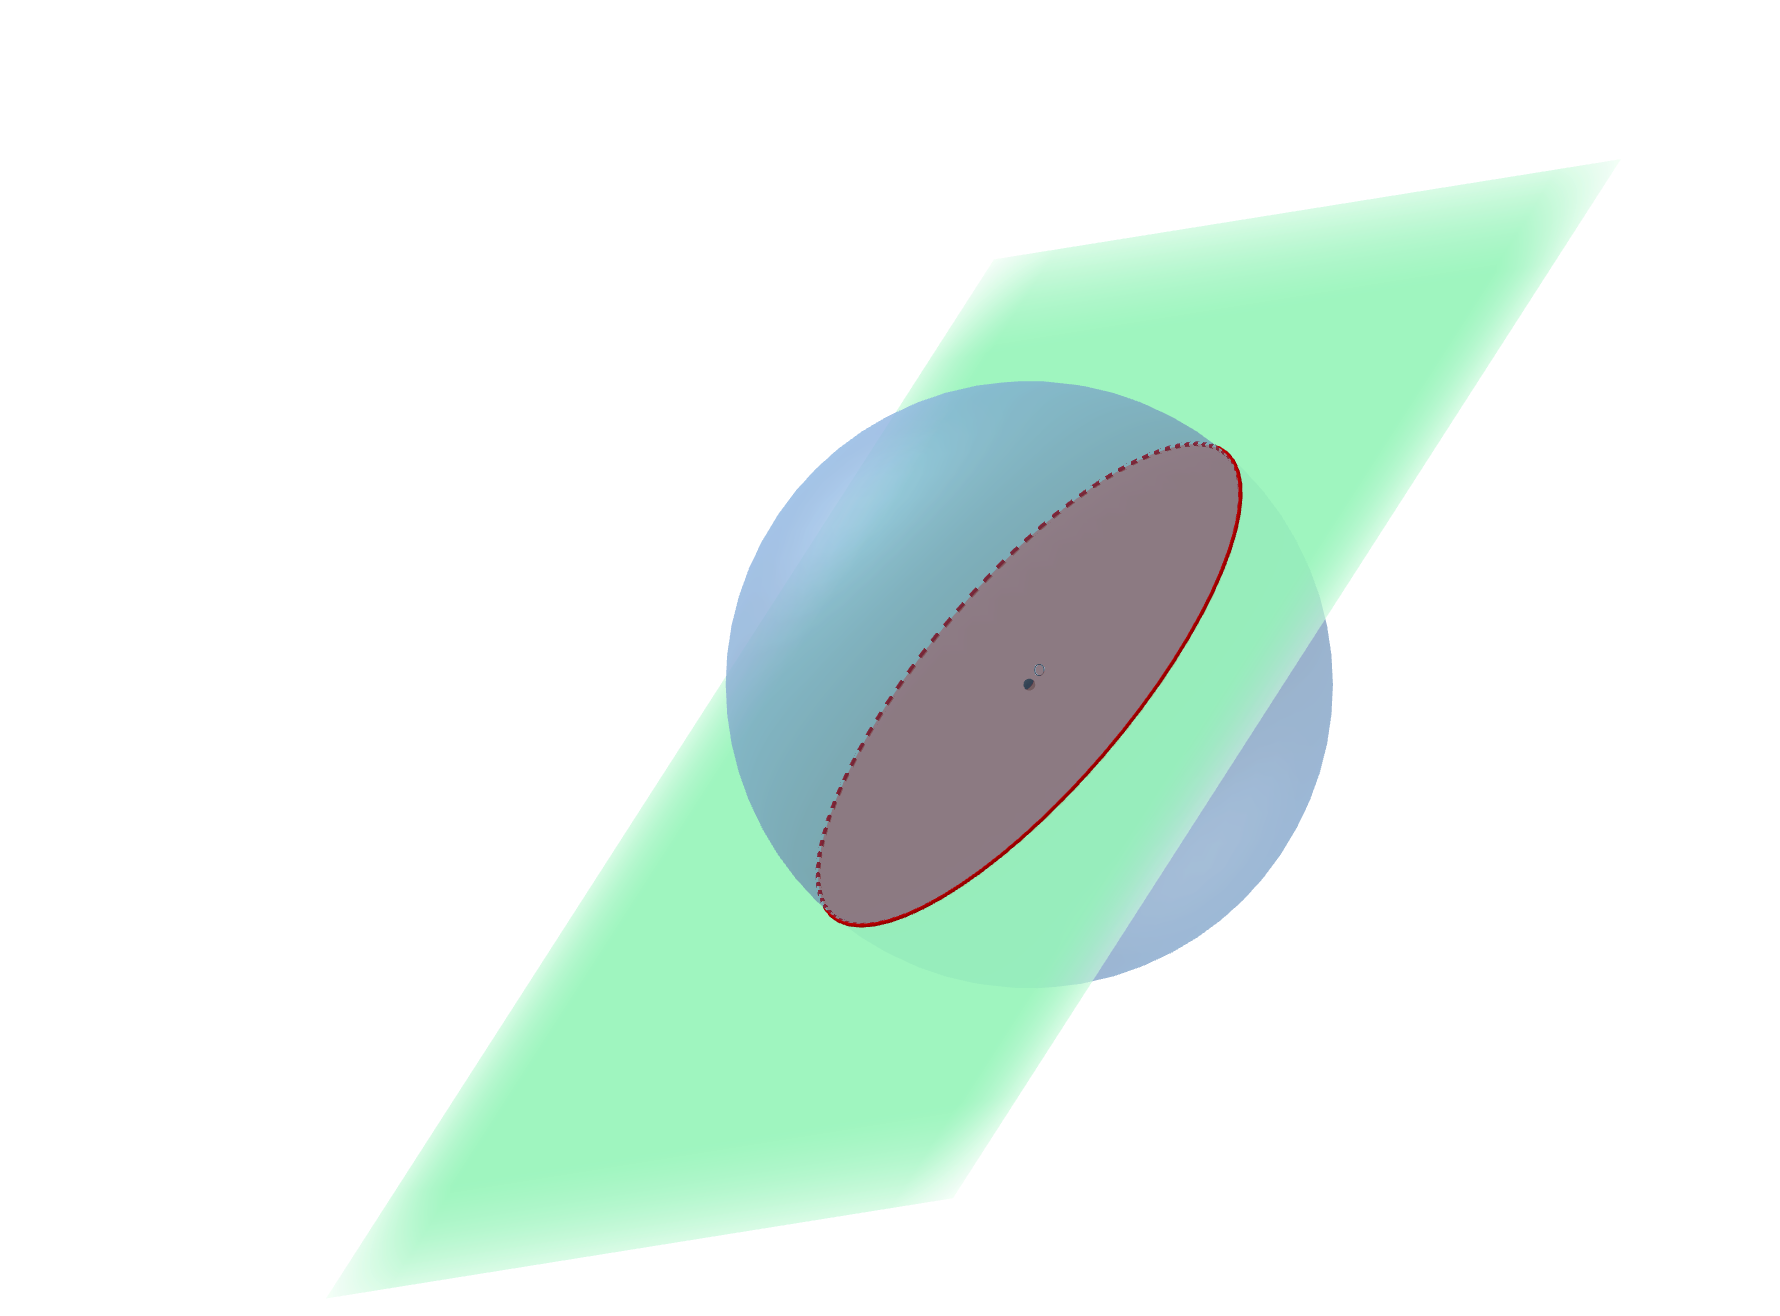
\includegraphics[trim={80 20 50 120}, clip, width=0.5\linewidth]{img/chapter_3/chiacchioellipsoid.png}
 \caption{Chiacchio's force ellipsoid expressed in the torque space (in red) (\cite{chiacchioForcePolytopeForce1997}). The feasible torques (in blue) are modeled as a ball of radius 1. The intersection with $\im J^T$ (green plane) produces a lower-dimensional ellipsoid (in red) defining Chiacchio's force ellipsoid expressed in the torque space.}
 \label{fig:chiacchio_ellispoid}
\end{figure}

While providing a useful framework, Chiacchio's construction does not explicitly incorporate muscle considerations. However, such considerations can be integrated by adjusting the radius of the torque feasible sphere to align with experimental data, as done in (\cite{rezzougUpperLimbIsometricForce2021b}). This raises the question of whether this scaling process adequately captures the complex interplay between muscles and joint torques. To address this, we adopt a more comprehensive approach by considering all possible models for the force feasible set, aiming to derive general results applicable to any model choice.

In this broader context, the isometric force feasible set, $\mathcal{F}$, for a $p$-dimensional kinematic chain with $n$ degrees-of-freedom and $m$ muscles (where $p \leq n \leq m$) at a specific posture is defined as:
\begin{align*}
 \mathcal{F} = \left\{ \mathbf{f}\in\mathbb{R}^p \mid \exists \mathbf{t}\in \mathcal{T},\quad J^T\mathbf{f} = -L^T\mathbf{t} - \mathbf{G}\right\}
\end{align*}
where $J^T\in\mathbb{R}^{n \times p}$ is the transpose of the Jacobian matrix (mapping end-effector forces to joint torques), $L\in\mathbb{R}^{m \times n}$ is the lever-arm matrix (where $-L^T$ maps muscle tensions to joint torques), $\mathbf{G}\in\mathbb{R}^n$ is the gravitational torque vector, and $\mathcal{T}\subset \mathbb{R}^m$ is the set of possible muscle tension combinations.

It is easily seen that Chiacchio's ellipsoid, in its raw form, corresponds to the case in which: gravity is not considered; the tension feasible set $\mathcal{T}$ is a centered sphere in $\mathbb{R}^m$ of radius 1; and $-L^T$ is an orthogonal projection from the tension space to the torque space. In other words, there are many simplifying assumptions regarding how muscles act on joints. The general force feasible set formulation require the following assumptions: 1) the muscle geometry must be known to compute the lever arms in $-L^T$; 2) the minimal and maximal tensions of each muscle must be known to estimate the possible values taken by $\mathbf{t}$; and 3) the neuromuscular behavior should be understood to properly model the shape of $\mathcal{T}$. 

Indeed, in this framework, the tension feasible set can be viewed as a linear transformation of the set of all possible muscle activations. Since muscles may be activated according to the activation of neighbor muscles (a behavior termed \emph{muscular grouping}), or activated according to an agonistic-antagonistic relationship with another muscle, this is equivalent to assuming a pairwise relationship between muscles. Consequently, the global shape of the tension feasible set is determined by a linear transformation of the activation set.  

Figure \ref{fig:formula_} illustrates this construction geometrically.
\begin{figure}[!ht]
  \centering
  \captionsetup{justification=centering}
  \begin{tikzcd}
    \mathcal{F}' \subset \mathbb{R}^p & \mathcal{F} \subset \mathbb{R}^n \arrow[l] \arrow[l, "(J^T)^+"] & \mathcal{T}_o\subset \mathbb{R}^n \arrow[l, "\cap \im J^T"] & \mathcal{T}\subset \mathbb{R}^m \arrow[l, "-L^T - \mathbf{G}"]
  \end{tikzcd}
  \caption{Description of the geometric operations to derive the force feasible set in isometric conditions. The set of muscle tensions $\mathcal{T}$ is projected and translated onto the torque space to create the torque feasible set $\mathcal{T}_o$. It is then intersected with a vector space ($\im J^T$) to produce the force feasible set $\mathcal{F}$ described in the torque space, or conveniently in the Cartesian force space using $(J^T)^+$. In practice, we prefer to express $\mathcal{F}$ in the torque space since $(J^T)^+$ is a bijection between $\mathcal{F}$ and $\mathcal{F}'$.}
  \label{fig:formula_}
\end{figure}

A straightforward application of this general formula arises when all muscles are considered fully activable simultaneously. In this scenario, the tension feasible set $\mathcal{T}$ is a linear transformation of a cube, resulting in an \emph{orthotope} (or hyperrectangle). This orthotope is then projected onto the torque space, producing a zonotope that represents all feasible torques. Consequently, the force feasible set, formed by the intersection of this zonotope with $\im J^T$, is a polytope.  We refer to this model, with the orthotopic assumption on the tension feasible set, as the $\mathcal{T}_{\infty}$ model.  Alternatively, if $\mathcal{T}$ is a linear transformation of a sphere (resulting in an ellipsoid), we call it a $\mathcal{T}_2$ model. In this chapter, we will consider a broader class of possible models, denoted $\mathcal{T}_p$, for $2 \leq p < +\infty$. Figure \ref{fig:tension_models} illustrates these two first models.
\begin{figure}[!htb]
  \centering
  \captionsetup{justification=centering}
  \begin{minipage}{0.49\linewidth}
    \centering
    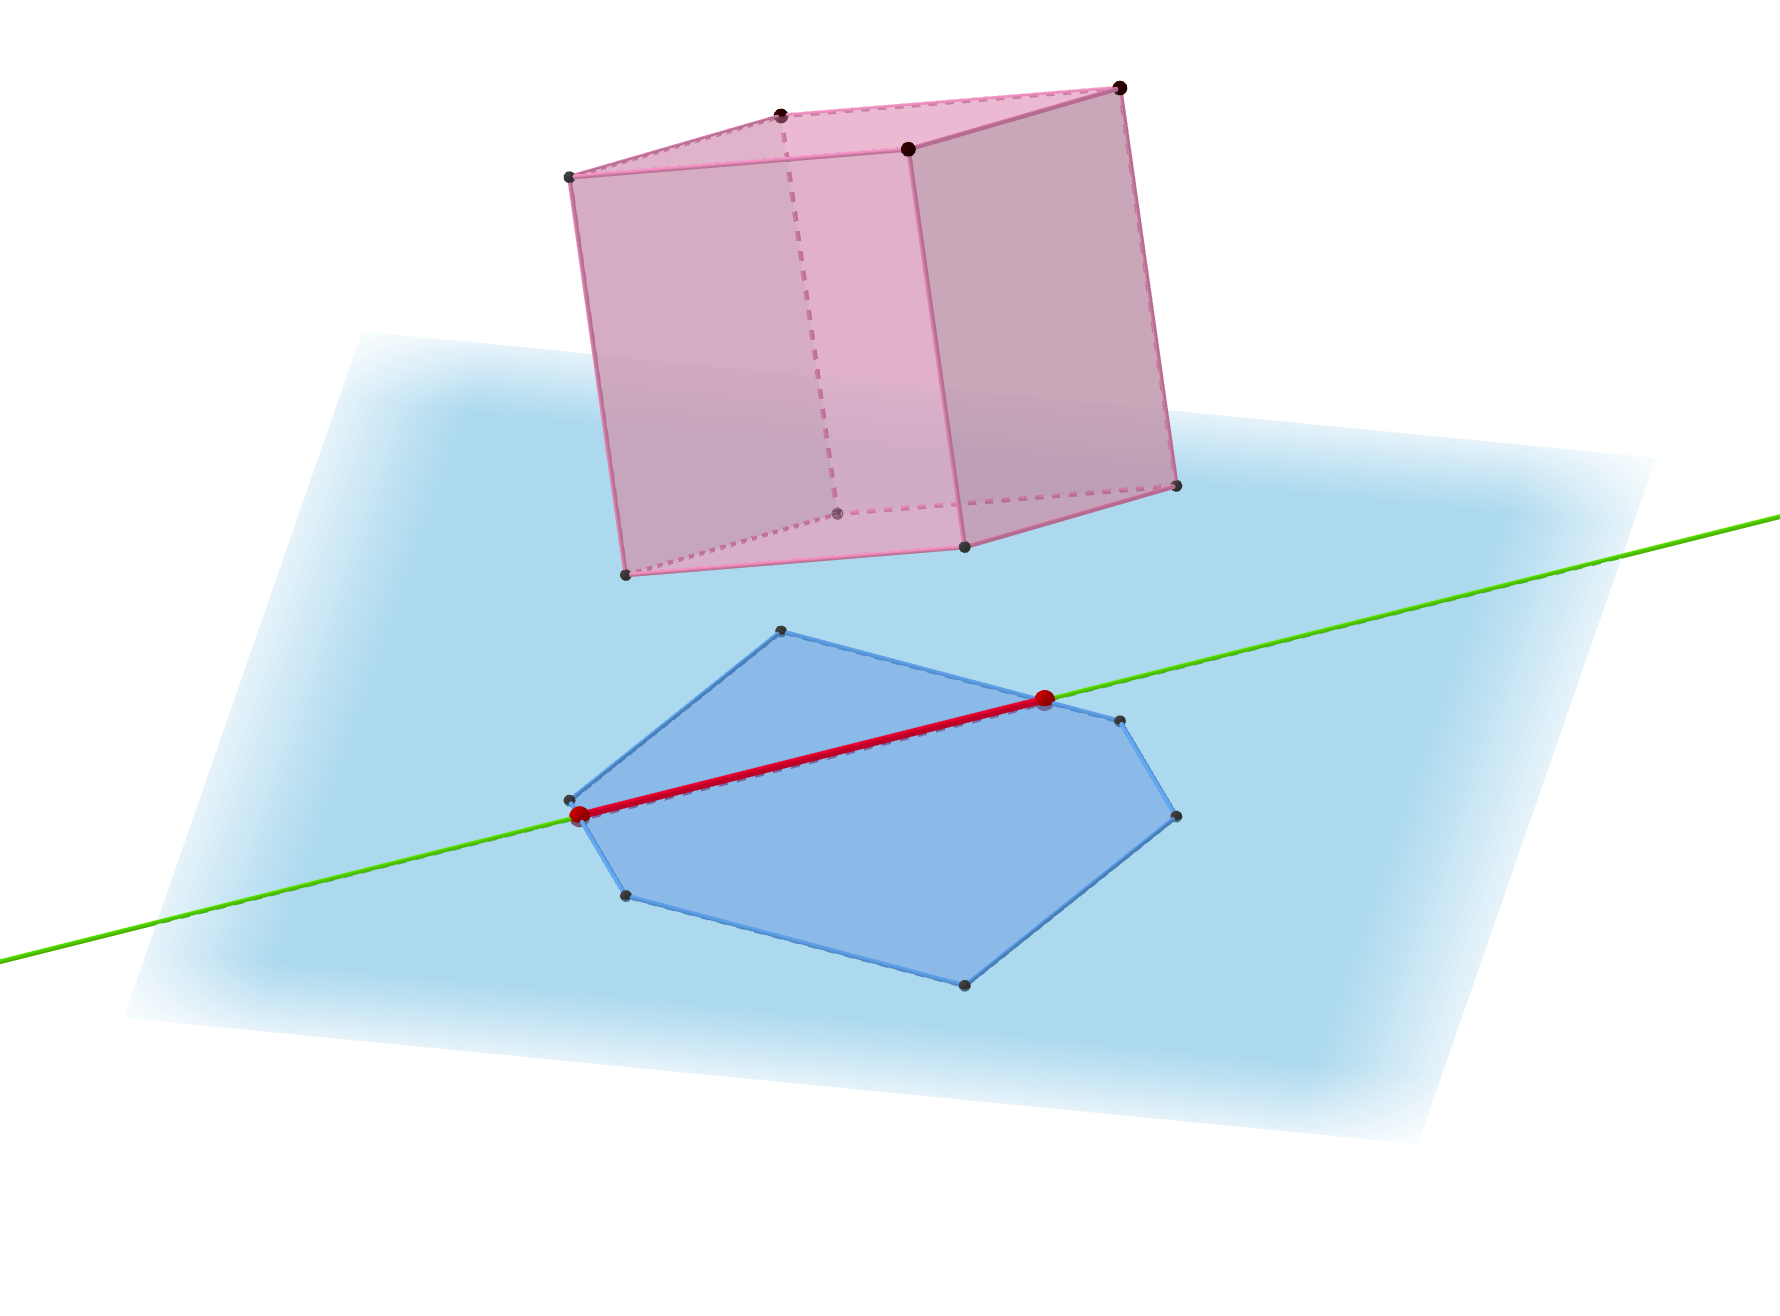
\includegraphics[trim={50 150 50 70}, clip, width=1\linewidth]{img/chapter_3/polytope_better_ggb.png}
  \end{minipage}
  \hfill
  \begin{minipage}{0.49\linewidth}
    \captionsetup{justification=centering}
    \centering
    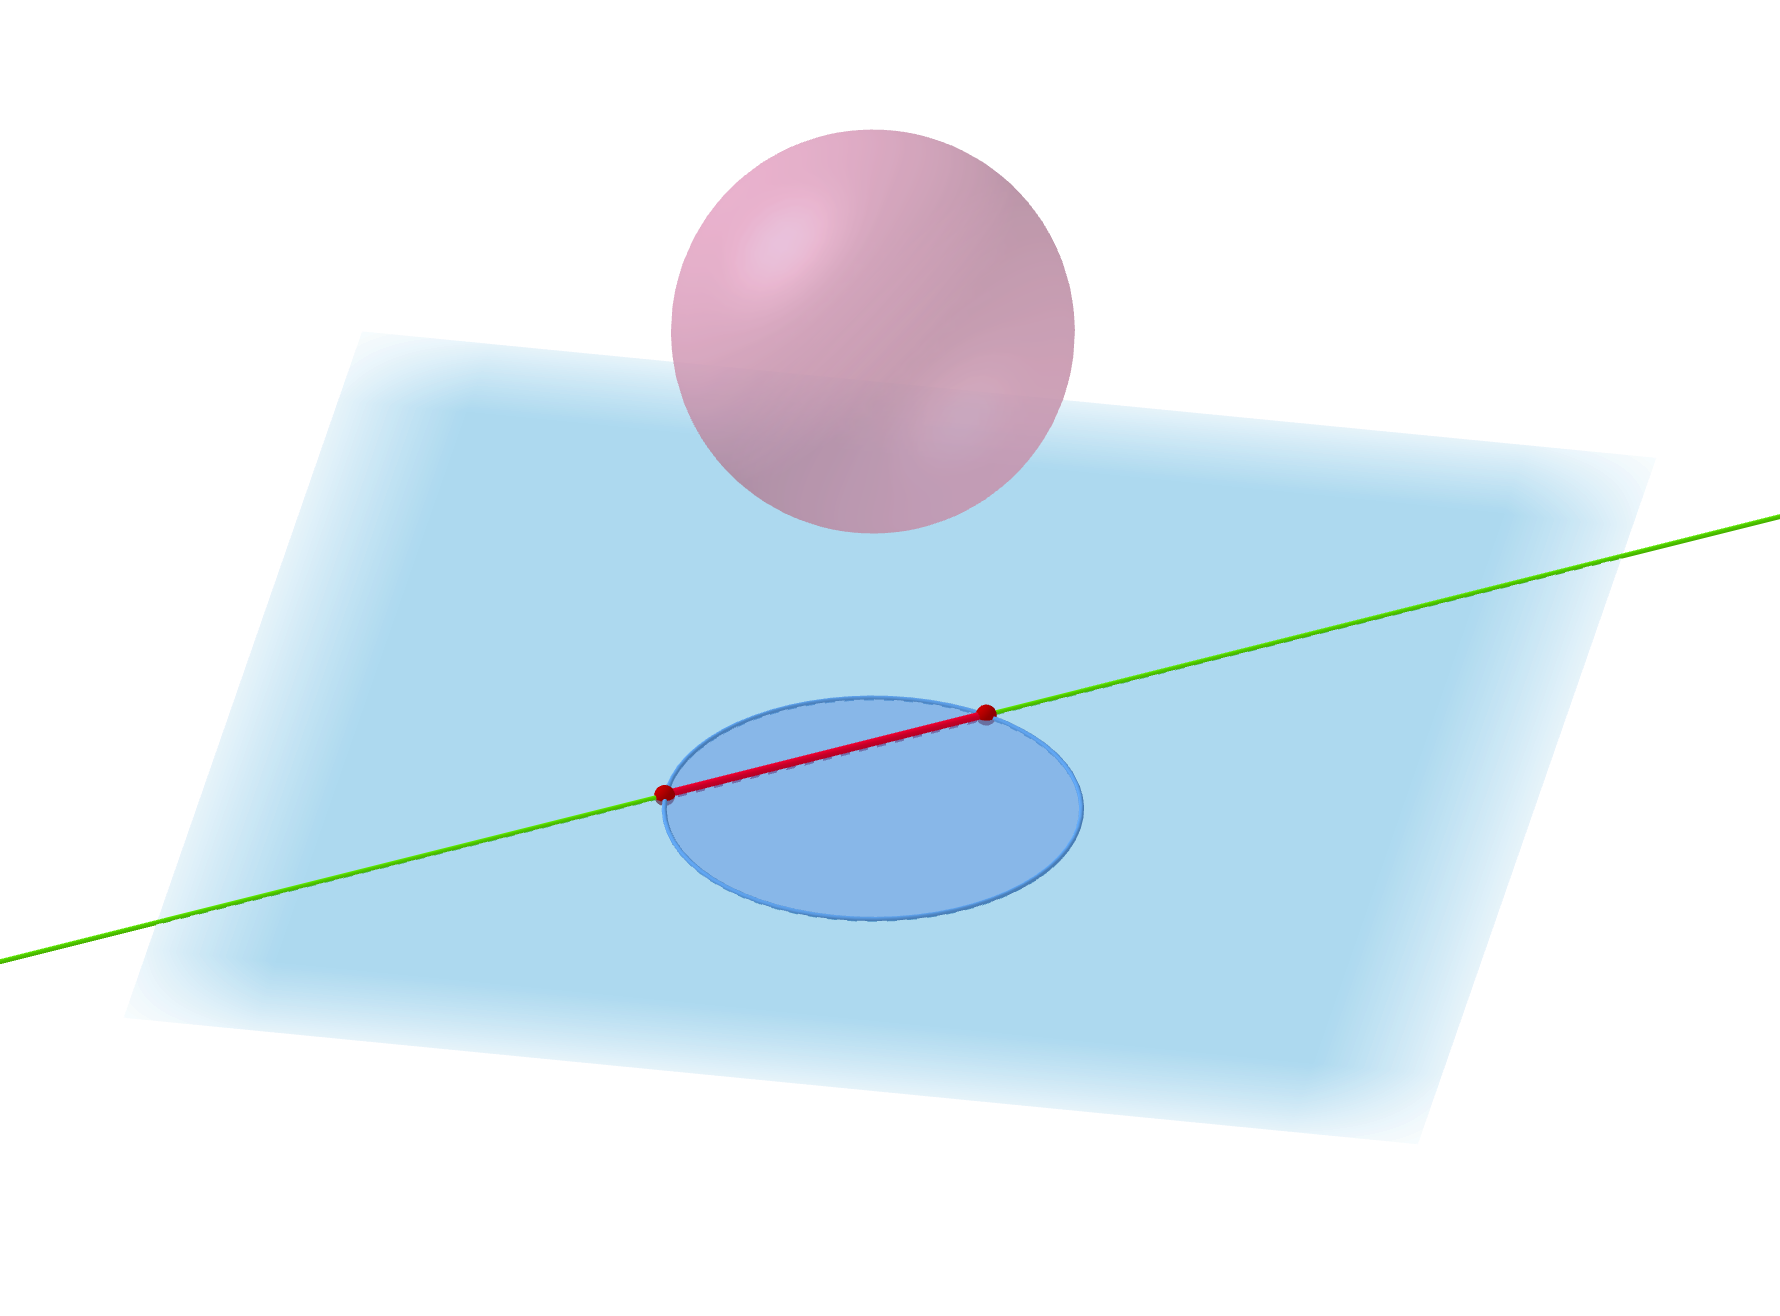
\includegraphics[trim={50 150 50 70}, clip, width=1\linewidth]{img/chapter_3/polytope_from_sphere_ggb.png}
  \end{minipage}
  \caption{Differences in the shape of the force feasible set $\mathcal{F}$ (in red) based on the modeling choice for the tension feasible set $\mathcal{T}$ (in pink). A $\mathcal{T}_{\infty}$ model implies that $\mathcal{T}$ is a linear transformation of a cube (an orthotope), while a $\mathcal{T}_2$ model is the linear transformation of a sphere (an ellipsoid). The force feasible set $\mathcal{F}$ can be constructed in two steps: first, $\mathcal{T}$ (pink) is projected onto the torque space (light blue plane), forming the torque feasible set $\mathcal{T}_o$ (dark blue). Then, $\mathcal{T}_o$ is intersected with a subspace (green line). All elements in this intersection constitute the force feasible set $\mathcal{F}$ described in the torque space.}
  \label{fig:tension_models}
\end{figure}

However, experimental measurements of maximal force exertions at the hand suggest that a scaled Chiacchio's ellipsoid ($\mathcal{T}_2$ model) underestimates these measurements, while the polytope ($\mathcal{T}_{\infty}$ model) overestimates them (\cite{rezzougUpperLimbIsometricForce2021b}). These estimations, based on in silico force feasible sets, required scaling a generic upper limb musculoskeletal model.
\begin{figure}[!htb]
  \captionsetup{justification=centering}
    \centering
    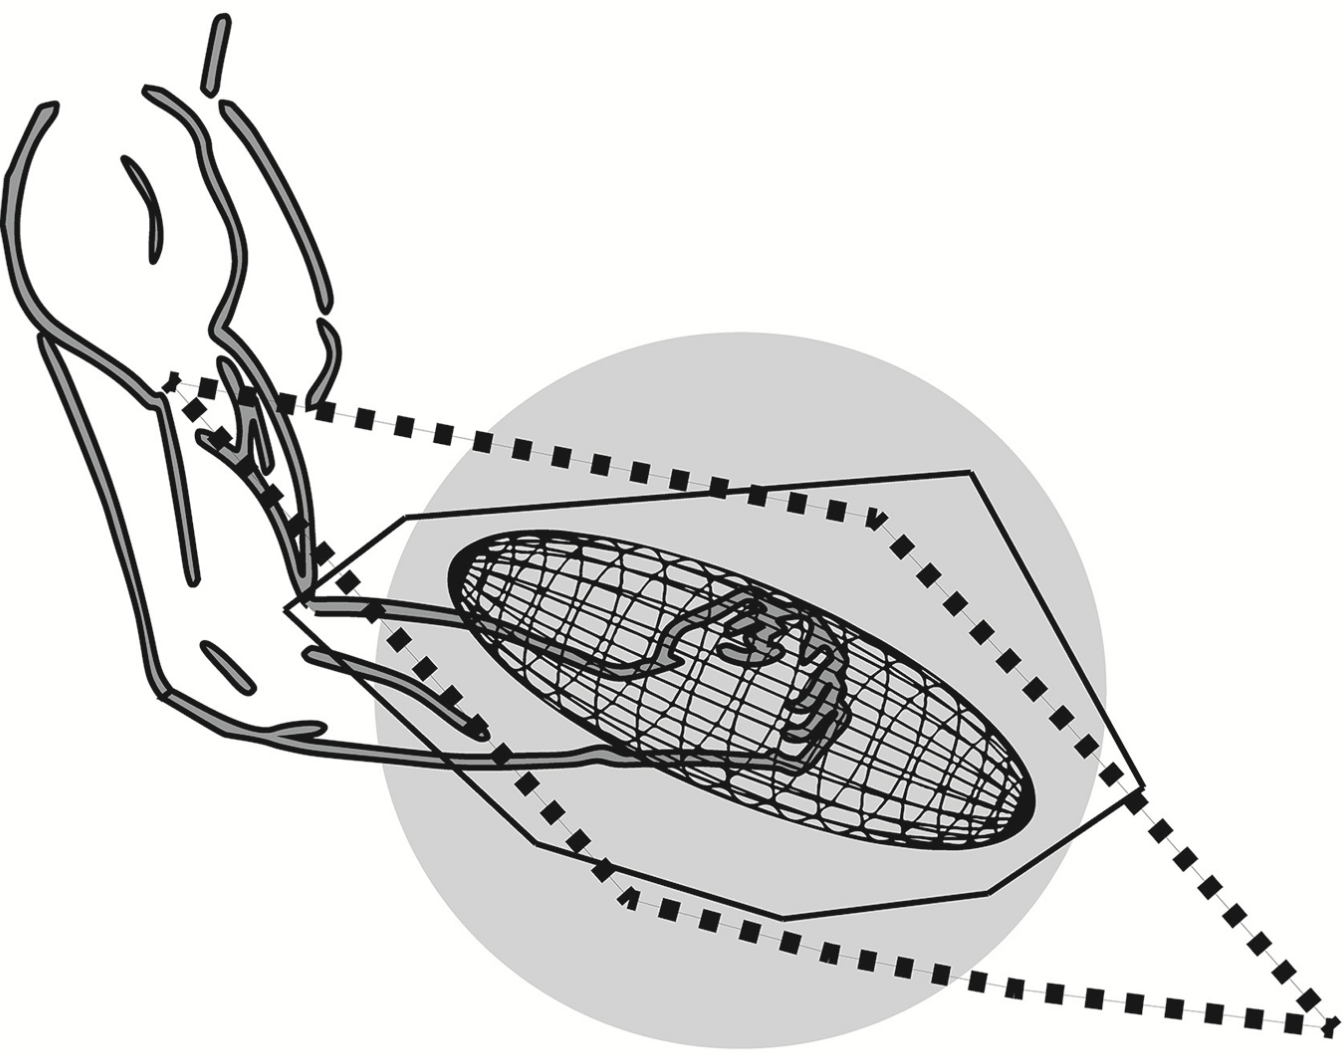
\includegraphics[trim={0 0 0 0}, clip, width=0.5\linewidth]{img/chapter_3/FFSComparisonRezzoug.png}
  \caption{Two modeled scaled force feasible set boundaries compared to experimental data, expressed in the sagittal plane relative to the upper-limb posture of one participant. The solid line represents the convex hull of experimentally measured maximal force exertions. The black squares depict the in silico force feasible set modeled as a polytope ($\mathcal{T}_{\infty}$ model), while the wire-frame represents the ellipsoid version ($\mathcal{T}_2$ model). The gray circle has a radius of 300N. Image extracted from (\cite{rezzougUpperLimbIsometricForce2021b}).}
  \label{fig:rezzoug_exp}
\end{figure}

Consequently, neither an ellipsoid nor a polytope representation of the force feasible set appears to fully capture the size of measured experimental force exertions. However, they seem to approximate the global orientation of the measured data. Since Chiacchio's ellipsoid does not require knowledge of muscle lever arms, it can be inferred that the Jacobian matrix, $J^T$, plays a crucial role in determining this orientation.

In the aforementioned representations of $\mathcal{F}$, the specific models share one common characteristic: $\mathcal{T}$ is assumed to be convex and symmetric. Most results in this chapter assume symmetry of the tension feasible set, $\mathcal{T}$, which might not always be realistic in a biomechanical context. They are valid for a broad class of nested symmetric shapes, which allows us to consequently extend the results to non-symmetric convex models that can be enclosed in between two arbitrarily chosen symmetric $\mathcal{T}$ shape models. This ensures applicability to a wide range of muscle activation patterns, even those that exhibit some degree of asymmetry. While a spherical shape offers computational advantages, it underestimates the true size of the force feasible set. Conversely, a cubical shape leads to combinatorial challenges, overestimates the size, and introduces unrealistically sharp edges in the context of human biomechanics.

This chapter aims to address these limitations through a deeper understanding of the mathematical formulation of force feasible sets. Our objectives are threefold:
\begin{enumerate}[noitemsep]
  \item \textbf{Decouple size and shape:}  Separate the notions of \emph{size} and \emph{shape} in $\mathcal{F}$ to gain finer control when fitting in silico models to experimental data (cf. Chapter \ref{chapter:5}). We will demonstrate that $\mathcal{F}$ inherently possesses an ellipsoidal shape, regardless of the chosen model, and that this approximation improves with the number of muscles considered.  Furthermore, we will show that the size of $\mathcal{F}$ depends on a coupling between the mean value of maximal muscle tensions and muscle path geometry.
  \item \textbf{Quantify the impact of muscle path geometry:} Analyze how muscle path geometry influences $\mathcal{F}$, and apply this analysis to determine whether personalization of muscle geometry in a scaled generic musculoskeletal model is necessary.
  \item \textbf{Provide modeling guidelines:} Offer insights into how force feasible sets should be modeled depending on the specific context.
\end{enumerate}

To achieve these goals, we seek the most suitable force feasible set model with size and shape consistent with experimental maximal force measurements in isometric conditions. Since these properties depend on the model chosen for the tension feasible set, we consider the class of all convex, symmetric sets for $\mathcal{T}$. This analysis utilizes the theory of Banach spaces (Section \ref{sec:theory_banach_spaces}), which provides a framework for treating symmetric convex sets as vector spaces equipped with a notion of size.

Section \ref{sec:ellipsoidal_shape_ffs} delves into the \emph{Local Theory of Banach spaces} to demonstrate that, irrespective of the choice of model for $\mathcal{T}$, the force feasible set tends to resemble an ellipsoid with high probability. This probability approaches 1 as the number of considered muscles increases, highlighting the role of the geometric construction of $\mathcal{F}$. This section concludes with a computationally amenable reformulation of the general description of $\mathcal{F}$ directly in the tension space, facilitating the analysis of how muscle tension combinations contribute to the force feasible set. While the ellipsoidal approximation is theoretically sound, its computation remains challenging and model-dependent. To overcome this, Section \ref{sec:projected_volume_problem} explores the projection constant theory within the Banach space framework. We show that the problem of fitting the size of $\mathcal{F}$ is directly linked to the choice of model for $\mathcal{T}$ and we propose an explicit computation for an adapted ellipsoid.

Building on the theoretical tools developed in the preceding sections, Section \ref{sec:sensitivity} introduces a novel index quantifying the influence of muscle path geometry (locations of path points and via points) on the force feasible set. This index, independent of the specific model chosen for $\mathcal{T}$, provides valuable insights into whether detailed personalization of muscle geometries is required when scaling a generic musculoskeletal model.

This chapter concludes by summarizing the theoretical analysis of the force feasible set, laying the foundation for the applications explored in the next two chapters, which focus on musculoskeletal model muscle personalization based on the knowledge of \emph{in silico} and \emph{in vivoe} force feasible sets in different postures.

\section{The theory of Banach spaces}
\label{sec:theory_banach_spaces}
This thesis adopts a set-theoretic approach to model the forces exertable by an individual. While intuitive for defining these sets, this approach may seem less practical when comparing force feasible sets between individuals or analyzing the influence of muscle tensions and geometry. To gain a more comprehensive understanding, we shift our perspective while retaining the underlying set-based vision. This section introduces the fundamentals of \emph{Banach spaces}, providing a structured framework for studying the geometry of symmetric convex sets and how unit metrics transform. This framework is based on the principle that \emph{in vivo} force feasible sets should reflect, in a structured manner, how muscle tensions interact. The specific structural properties will thus be thoroughly studied in this chapter to gain insights into muscle feasible tensions and their interactions directly from the force feasible sets.

\paragraph*{Banach space.} A \emph{complete normed vector space} is called a Banach space.  Completeness implies that every Cauchy sequence in the space converges to a limit within that space, ensuring no "gaps" or "missing points."  A normed space is equipped with a notion of \emph{size} for each element $x$, called the \emph{norm of x}, denoted by $\|x\|_X$ (the subscript may be omitted when the context is clear). Formally, a Banach space is often denoted as $(X,\, \|\cdot \|_X)$. This thesis focuses on \emph{finite-dimensional real-valued normed} vector spaces, where vectors have a finite number of real-valued components.  Such spaces are inherently complete and thus qualify as Banach spaces.

We present two complementary perspectives on Banach spaces:

\begin{enumerate}
  \item{ \textbf{Geometric perspective:} Visualize a Banach space as a vector space containing a centrally symmetric convex set centered at the origin. This set, often referred to as the \emph{unit ball}, can be a sphere, ellipsoid, zonotope, cube, or any other fully-dimensional, centrally symmetric convex set.  Transformations between Banach spaces not only map the underlying vector space but also "deform" the unit ball into another convex set.}
  \item{ \textbf{Metric perspective:}  Interpret a Banach space as a vector space with a well-defined notion of a \emph{unit metric system}. This allows us to study how a unit of measurement transforms under different mappings.}
\end{enumerate}

These two perspectives allow us to draw a parallel between the geometric properties of the force feasible set and its physical interpretation. The choice of perspective depends on the context. For instance, we will demonstrate that force feasible sets tend to resemble ellipsoids when a large number of muscles are involved. This result is established by analyzing how the Newton unit, used to quantify muscle tension combinations, undergoes a quadratic transformation to become the Newton-meter unit in the torque space.

While this thesis assumes a familiarity with linear algebra, the geometric and metric perspectives on Banach spaces may be less familiar, particularly in higher dimensions. For an intuitive understanding, we encourage the reader to primarily adopt the geometric viewpoint for now. The following paragraphs introduce fundamental concepts that form the basis of any study on Banach spaces.

\paragraph*{The $p$-norms and $\ell_p^n$ spaces.} Norms provide tools for measuring the \emph{size} of elements in a vector space. In $\mathbb{R}^n$, a common norm is the Euclidean norm (or 2-norm), defined as $\|\mathbf{x}\|_2 = \sqrt{x_1^2 + \dots + x_n^2}$. When $\mathbb{R}^n$ is equipped with $\|\cdot \|_2$, we refer to it as $n$-dimensional Euclidean space. However, other norms can be defined on $\mathbb{R}^n$.  The $p$-norm, denoted by $\|\cdot \|_p$, is given by:
\begin{align*}
\|\mathbf{x}\|_p = \left(\sum_{i=1}^n \vert x_i \vert^{p}\right)^{1/p}
\end{align*}

The Euclidean norm is a special case of the $p$-norm with $p=2$.  Another useful norm is the $\infty$-norm, defined as:
\begin{align*}
\|\mathbf{x}\|_{\infty} = \lim_{p\to \infty} \|\mathbf{x}\|_p = \max_{i=1,\dots,n}\vert x_i\vert
\end{align*}

Each $p$-norm provides an analytical description of the geometry of a specific type of centrally symmetric convex set.  The surface of such a set can be represented as $\{\mathbf{x}\in \mathbb{R}^n \mid \|\mathbf{x}\|_p = 1\}$.  This analytical representation is valuable for our purpose of analyzing and fitting the shapes of force and torque feasible sets.

To clearly indicate which $p$-norm is being used, we adopt the notation $\ell_p^n$ to represent the $n$-dimensional real vector space $\mathbb{R}^n$ equipped with the $p$-norm $\|\cdot \|_p$.

\paragraph*{Unit balls.} A norm quantifies the elongation of a vector relative to a reference value that depends on its direction and the dimension of the ambient space. Similarly, the amplitude of a maximal isometric force exerted at the hand depends on the direction of force application. Choosing a norm for a Banach space $X$ effectively defines how different directions in $X$ influence the elongation of a vector. To capture all possible influences (since there are infinitely many directions for $n \geq 2$), we consider the set $\mathcal{B}_X = \{\mathbf{x}\in X \mid \|\mathbf{x}\|_X \leq 1 \}$, called the \emph{unit ball} of $X$.  For $\ell_p^n$ spaces, we denote their unit balls by $\mathcal{B}_p^n$, as illustrated in Figure \ref{fig:pnorms} for $\ell_p^2$ spaces with various values of $p$.

\begin{figure}[!htb]
  \captionsetup{justification=centering}
    \centering
    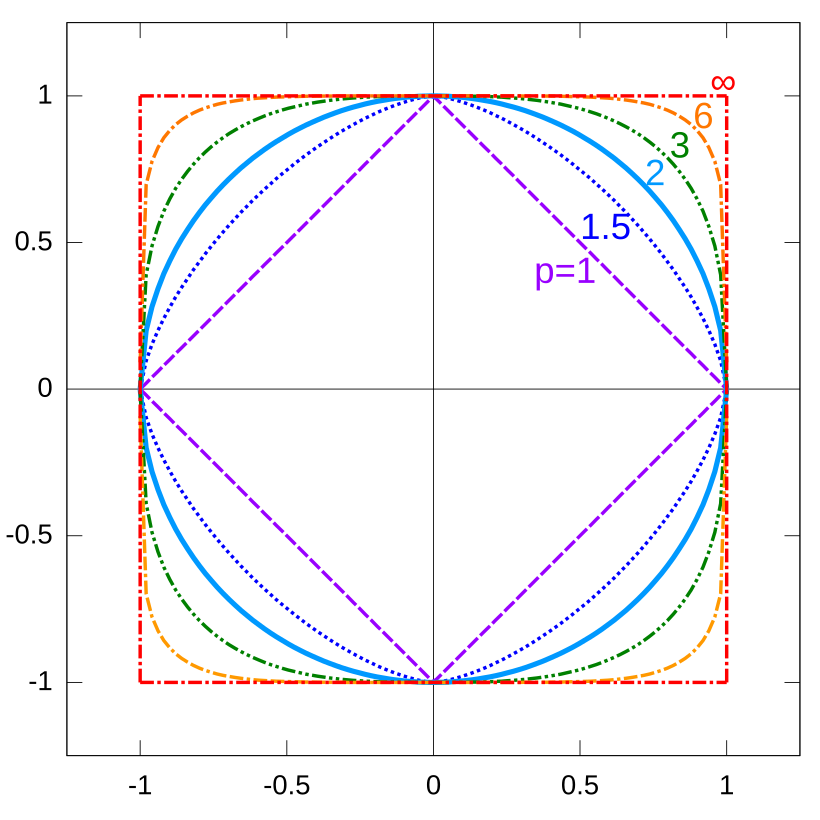
\includegraphics[trim={0 0 0 0}, clip, width=0.4\linewidth]{img/chapter_3/p_norms.png}
  \caption{Unit balls associated with different $p$-norms in $\mathbb{R}^2$ (from Wikipedia).}
  \label{fig:pnorms}
\end{figure}

% \paragraph*{Symmetric convex sets and $p$-unit balls.}
% In figure \ref{fig:pnorms}, we can see that the most convenient $p$-norm to work with is $p=2$, the euclidean norm: the notion of size in the considered space is the same in any direction (all directions matter). If we consider $p=\infty$, then we are saying that only the principal direction of a vector matters (\emph{i.e.} its largest component in absolute value). Generalizing these interpretations for $2< p <\infty$, the more large $p$ gets, the more importance is given to the principal direction of a vector. A contrario, the more close to $2$ $p$ gets, the less distinction we make between important directions. This is geometrically represented by \emph{how rounded} the unit ball $\mathcal{B}_p^n$ is, with $\mathcal{B}_2^n$ being a purely rounded ball of radius 1 in $\IRn$ and $\mathcal{B}_{\infty}^n$ being a $n$-dimensional cube centered at origin whose edges are of length $2$. Unit balls $\mathcal{B}_p^n$ are necessarily symmetric around the origin of $\IRn$.

% The point of view we are giving to the reader is thus the following: studying $p$-norms of $\IRn$ corresponds to studying the symmetric convex set associated to their unit balls. This is interesting in theory, but there is not much we can do with this.

\paragraph*{Operators.} Let $X$ and $Y$ be Banach spaces with norms $\|\cdot\|_X$ and $\|\cdot\|_Y$ respectively. An \emph{operator} $T: X \rightarrow Y$ is a continuous linear map between $X$ and $Y$. Operators transform Banach spaces into Banach spaces. Linearity ensures that a vector space is mapped to a vector space, while continuity preserves completeness, guaranteeing that the resulting space after the transformation remains "whole" with no "gaps" or "missing points."

In finite dimensions, any operator $T: X \rightarrow Y$ can be represented by a matrix. However, this matrix representation only captures how the vector space structure of $X$ is transformed under $T$. We need a more comprehensive tool to study how the norm of $X$ is affected by $T$. Since the norm structure of $X$ is characterized by its unit ball, the key question becomes: \emph{How is the unit ball of $X$ transformed by $T$?}

To answer this, we need to consider the properties of $T$. An operator $T: X \rightarrow Y$ is \emph{bounded} if $T(\mathbf{x})$ is bounded for all $\mathbf{x} \in \mathcal{B}_X$.  Since a linear map between normed spaces is continuous if and only if it is bounded, $T$ must be bounded. This implies that the set of operators from $X$ to $Y$ forms a Banach space, which can be equipped with a norm called the \emph{operator norm}, defined as:
\begin{align*}
\|T\|_{op} = \sup\left\{\|T(\mathbf{x})\|_Y \mid \mathbf{x}\in \mathcal{B}_X \right\}
\end{align*}

The operator norm has a clear geometric interpretation: it represents the largest distance between the transformed unit ball of $X$,  $\{T(\mathbf{x}) \mid \mathbf{x}\in \mathcal{B}_X\}$, and the unit ball of $Y$, as depicted in Figure \ref{fig:operator_norm}.
\begin{figure}[!htb]
  \captionsetup{justification=centering}
    \centering
    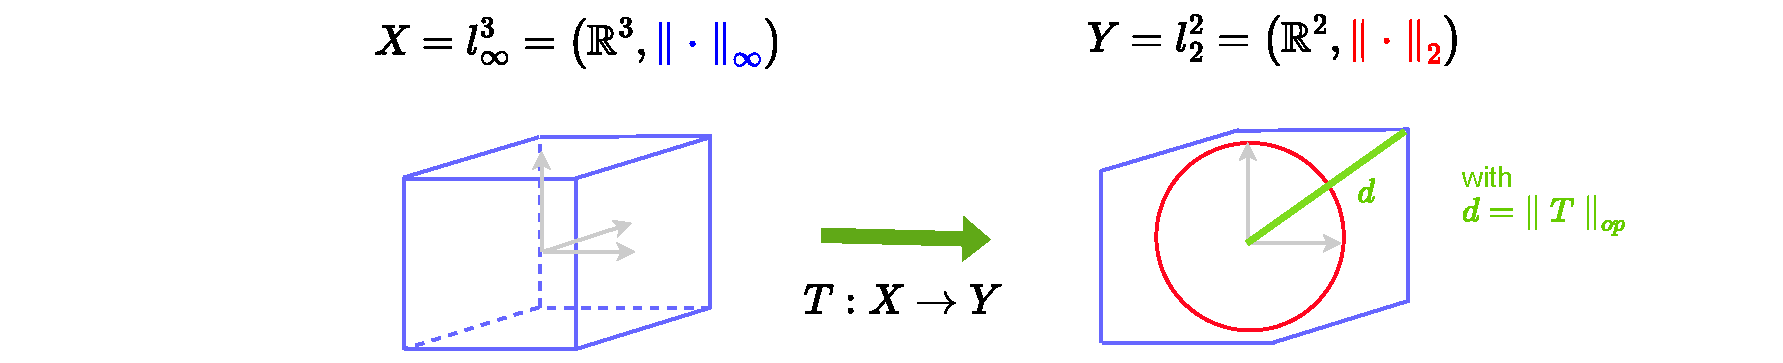
\includegraphics[trim={150 0 70 0},clip, width=1\linewidth]{img/chapter_3/operator_norm.pdf}
  \caption{Geometric interpretation of the operator norm. $T$ projects $\ell_{\infty}^3$ onto $\ell_2^2$. Its operator norm, $\|T\|_{op}$, is the maximal Euclidean norm of the vectors describing the surface of the projected unit ball of $\ell_{\infty}^3$. In this case, this corresponds to the surface of a zonotope (blue). This is equivalent to computing the maximal 2-norm of the zonotope vertices.}
  \label{fig:operator_norm}
\end{figure}

In essence, the operator norm quantifies the maximal deformation of the transformed unit ball of $X$ relative to the unit ball of $Y$. With this understanding, we are now equipped to delve into the comparison of centrally symmetric convex sets.

\paragraph*{Banach-Mazur distance.} Consider two isomorphic Banach spaces $X$ and $Y$, meaning there exists an invertible linear map between them. Recall that two finite-dimensional real vector spaces are isomorphic if and only if they have the same dimension. In this case, their \emph{Banach-Mazur distance} is defined as:
\begin{align*}
d_{BM}(X,Y) = \inf\{\|T\|_{op} \|T^{-1}\|_{op} \mid T: X\rightarrow Y \text{ is an isomorphism}\}
\end{align*}

If $X$ and $Y$ are not isomorphic, we define $d_{BM}(X,Y) = +\infty$.

When the Banach-Mazur distance is 1, $X$ and $Y$ are said to be \emph{isometric}, meaning they have the same metric structure up to isomorphism. This implies that the set of points at a distance of 1 from the origin in $X$ corresponds exactly to the set of points at a distance of 1 from the origin in $Y$. More generally, as noted in (\cite{milmanDvoretzkyTheoremThirtyYearsLater1992}), for two finite-dimensional real spaces $X$ and $Y$ of the same dimension with respective unit balls $\mathcal{B}_X$ and $\mathcal{B}_Y$, if $d_{BM}(X,Y) \leq d$, then there exists an operator $T: X \rightarrow Y$ such that:
\begin{align*}
\mathcal{B}_X \subset T(\mathcal{B}_Y) \subset d \cdot \mathcal{B}_X
\end{align*}

This means that a linear transformation of the unit ball of $Y$ can be enclosed by the unit ball of $X$ and its dilation by a factor of $d$. Throughout this chapter, we will focus on cases where the unit ball of $X$ is an ellipsoid (so $X = \ell_2^n$), and the unit ball of $Y$ (representing the muscle tension space or the Cartesian force space) is enclosed by an ellipsoid, with $d$ being as close to 1 as possible.

\begin{figure}[!htb]
  \captionsetup{justification=centering}
    \centering
    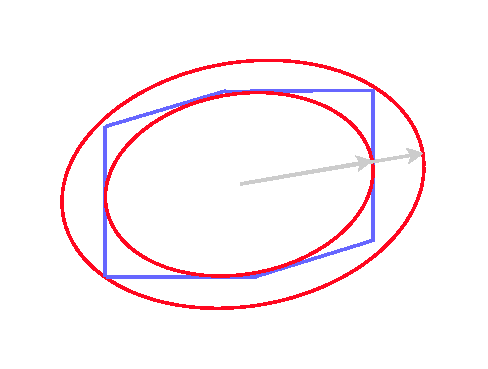
\includegraphics[trim={0 25 0 25},clip, width=0.5\linewidth]{img/chapter_3/banachmazurdvoretzky.pdf}
  \caption{Building on Figure \ref{fig:operator_norm}, we observe that the projected zonotope lies between a transformation of the disk (an ellipsoid) and a dilation of this ellipsoid by a factor of 1.4. This implies that $d_{BM}(Y, T(X)) \leq 1.4$.}
  \label{fig:banach_mazur_example}
\end{figure}

While the Banach-Mazur distance is a theoretical tool and often cannot be explicitly computed, it will be instrumental in demonstrating strong approximation results in high dimensions in the following sections.

This overview of Banach spaces has introduced mathematical tools for studying centrally symmetric convex sets. This structural approach yields valuable insights, which we will explore in the subsequent sections. With the sole assumption that the tension feasible set is symmetric and convex, we will demonstrate that the \emph{shape} of the force feasible set is largely independent of the specific model chosen for the tension feasible set, while its \emph{size} is model-dependent.

Leveraging the \emph{Local Theory of Banach spaces}, Section \ref{sec:ellipsoidal_shape_ffs} argues that the force feasible set inherently tends to be ellipsoidal due to its geometric construction.  However, in practice, we need to compute this ellipsoidal shape. Section \ref{sec:projected_volume_problem} utilizes the \emph{Projection Constant Theory} to provide a computational tool for approximating the force and torque feasible sets as ellipsoids, taking into account volume changes associated with norm deformations.

% require more depth, in particular results in what it called the \emph{local theory of Banach spaces}, which focuses on studying infinite-dimensional Banach spaces using only finite-dimensional tools. In particular, we are interested in a major result stating that a specific geometric construction over an initial symmetrically convex set will lead to an ellipsoidal shape.

% , section \ref{sec:ellipsoidal_shape_ffs} will show that due to its geometric construction, the force feasible set has a high probability of resembling an ellipsoid. This result is fundamental because it applies \emph{whatever the choice of the tension feasible set shape}. Even better, this ellipsoidal shape \emph{has to} occur due to the small dimensions of the Cartesian force space and the torque space (which is very different from the other perspective on saying that it occurs du to the large amount of muscles). Section \ref{sec:leveraging_the_projected_volume} will dive much deeper in the \emph{projection constant theory}, including a much more theoretical analysis studying problems related to the projection of a physical unit metric onto a subspace. While these sections are underlyingly studying how convex sets are projected and how muscle tensions are deformed onto torques, the final result is a fast explicit computation of the ellipsoidal approximation of the force feasible set.

\section{The ellipsoidal shape of the force feasible set}
\label{sec:ellipsoidal_shape_ffs}
The results in this section are foundational to the \emph{Local Theory of Banach spaces} and provide a valuable theoretical framework. They enable a concise geometric characterization of the force feasible set without imposing specific assumptions on the shape of the tension feasible set $\mathcal{T}$, except for convexity and symmetry. We will leverage the symmetry assumption in certain cases.

We consider various models for the tension feasible set, denoted by $\mathcal{T}_p$, each associated with a linear transformation of a unit $p$-ball. A $\mathcal{T}_2$ model corresponds to a spherical shape, representing a scenario where all muscle activations are equally constrained. In contrast, a $\mathcal{T}_{\infty}$ model assumes a cubic shape, allowing for independent activation of each muscle. The remaining $\mathcal{T}_p$ models, with $2 < p < \infty$, represent intermediate cases with varying degrees of "roundedness":
\begin{align*}
\mathcal{T}_2 < \mathcal{T}_3 < \dots < \mathcal{T}_{100} < \dots < \mathcal{T}_{\infty}
\end{align*}

The central result of this section establishes the inherent \emph{ellipsoidal} nature of the force feasible set. This means that $\mathcal{T}_p \approx \mathcal{T}_2$ for any $p \geq 2$, and more generally, $\mathcal{T} \approx \mathcal{T}_2$ for any convex, symmetric tension feasible set. The term "ellipsoidal" emphasizes that the force feasible set resembles an ellipsoid globally but may not perfectly coincide with one. However, it can be effectively approximated by an ellipsoid that captures the essential features of its shape. Our goal is to compute this approximating ellipsoid (see Section \ref{sec:projected_volume_problem}), but first, we need to elucidate the underlying reasons for this phenomenon and the conditions under which such an approximation is valid.

Before delving into the mathematical details, let's highlight the advantages of an ellipsoidal representation. First, it offers a significantly more compact and computationally efficient description, requiring only the lengths of the principal axes, a center point, and an orientation. This contrasts with, for example, a polytope representation, which may involve numerous vertices and bounding hyperplanes. Second, if the force feasible set resembles an ellipsoid in any posture, it follows from geometric considerations that the torque feasible set and the tension feasible set also exhibit ellipsoidal shapes, given that ellipsoids are preserved under affine transformations. Consequently, the tension feasible set $\mathcal{T}$ can be effectively modeled as a $\mathcal{T}_2$ model, simplifying the analysis of muscle activation relationships. In this spherical representation, the size of the tension feasible set is primarily characterized by the mean of the maximal tension values.


The results presented in this section, drawn from the \emph{Local Theory of Banach spaces}, are non-trivial and require a basic understanding of Banach space concepts. They may initially seem counter-intuitive due to the high-dimensional spaces involved.

The Local Theory investigates infinite-dimensional normed spaces using tools from finite-dimensional normed spaces.  Over the past century, the name of this theory has evolved from \emph{Local Banach Theory} and \emph{Asymptotic Finite-Dimensional Analysis} to \emph{Probabilistic Geometry} and, more recently, \emph{Asymptotic Geometric Analysis} \cite{artstein-avidanAsymptoticGeometricAnalysis2015}. Regardless of the nomenclature, this theory provides insights into how symmetric convex sets can be approximated by other symmetric convex sets. From a metric perspective, it helps us understand how the physical unit of the tension feasible set (Newtons) transforms into the physical unit of the torque space (Newton-meters) when a large number of muscles are considered.

For a comprehensive overview of the Local Theory, we recommend exploring the diverse perspectives presented in (\cite{pietschWhatLocalTheory1999}). A viewpoint relevant to our context is articulated in page 5 of (\cite{tomczak-jaegermannBanachMazurDistancesFinitedimensional1989}):
\begin{quote}
  ``A property [...] is called \emph{local} if it can be defined by a quantitative statement or inequality concerning a finite number of vectors or finite-dimensional subspaces.''
\end{quote}

This section focuses on characterizing the \emph{shape} of the force feasible set, which is a \emph{global} property. The overall shape can be described by its curvature, which involves considering tangents at every point on the surface, an infinite set. In contrast, a local property involves only finite quantities. For instance, the \emph{size} of a vector is a local property, computable in a finite number of steps. Since this applies to any vector, the notion of size itself is a local property of the space. The Local Theory aims to bridge the gap between local and global properties, enabling us to understand global geometric features through local analysis. In our context, it will illuminate the shape of the force feasible set by examining how different notions of size are deformed between spaces.

Dealing with infinity often introduces counter-intuitive concepts and challenges our ability to visualize them geometrically. Similar challenges arise in sufficiently high-dimensional spaces. To prepare for this exploration, we adopt the paradigm articulated in (\cite{milmanRegularRandomSections2021}):
\begin{quotation}
  \centering
  ``Existence implies abundance.''
\end{quotation}

In essence, this means that if at least one element of a class of objects in a sufficiently high-dimensional space possesses a certain property, then all other elements in that class are likely to share that property. Of course, this does not hold for all properties. However, the Local Theory is grounded in the observation that the more complex a normed space, the more its structure resembles that of a Euclidean space. In other words, even if a normed space is equipped with a highly complex norm, it still exhibits the structure of a simpler space with an ellipsoidal norm. As we will demonstrate later in this section, the force feasible set can be reformulated to reveal its inherent ellipsoidal shape.
To guide the reader through the following steps, let's chronologically summarize the key results presented in this section:

\begin{enumerate}
  \item {\textbf{1961 Dvoretzky's Theorem (\cite{dvoretzkyTHEOREMCONVEXBODIES1961}):} This foundational result in the Local Theory of Banach spaces states that for a large $m$ and an $m$-dimensional centrally symmetric convex set, there exists at least one projection onto or intersection with an $n$-dimensional subspace such that the resulting object resembles an ellipsoid. The dimension $n$ depends on the desired accuracy of the approximation.}
  \item {\textbf{1971 Milman's abundance (\cite{milmanAsymptoticTheoryFinite2001}):}  Milman extended Dvoretzky's Theorem by demonstrating that the existence result holds not just for one subspace but for almost all $n$-dimensional subspaces with high probability. The term `high probability' refers to a probability that increases towards 1 as $m$ grows large.}
  \item {\textbf{1984 Milman's Quotient of Subspace (QS) Theorem (\cite{milmanAlmostEuclideanQuotient}):}  For a centrally symmetric convex set in $m$ dimensions, there exists a subspace of dimension $p$ (constructed through a projection followed by an intersection) that exhibits an ellipsoidal shape. The key contribution of this theorem is to show that the ellipsoidal shape depends on $p$, not on $m$, highlighting the role of the geometric construction (projection then intersection) in inducing the ellipsoidal shape.}
  \item {\textbf{2021 Milman and Yifrach's Quotient of Subspace abundance (\cite{milmanRegularRandomSections2021}):}  This work generalizes the original QS Theorem, which was an existence result, to show that it applies to almost all $p$-dimensional subspaces with high probability.}
\end{enumerate}
% \item { \textbf{1975 Larman and Mani's extension to non-central projection or section \cite{larmanAlmostEllipsoidalSections1975a}:} Dvoretzky's theorem concerns subspaces passing through the origin. Larman and Mani extended his result to a $n$-dimensional subspace passing through any interior point of a $m$-dimensional symmetric convex set. More precise results on the resemblance and how to generalize to abundance have been made by Gordon in 1988 \cite{gordonGaussianProcessesAlmost1988};}

In the context of this thesis, the first two theorems indicate that as the number of considered muscles increases, the force feasible set tends to become more ellipsoidal, with high probability. This also applies to the torque feasible set. The latter two theorems are even more relevant, as they demonstrate that the ellipsoidal shape is not merely a consequence of the number of muscles but rather an inherent result of the geometric construction itself. However, these theorems alone do not provide a concrete method for constructing an ellipsoidal approximation. This will be the focus of Section \ref{sec:projected_volume_problem}.

It is crucial to note that all the theorems mentioned are independent of the specific norm chosen. We do not impose any particular shape on the tension feasible set, only that it is centrally symmetric and convex.

The following paragraphs elaborate on these results and demonstrate how the geometric construction of the force feasible set can be adapted to align with the Quotient of Subspace Theorem. While the proofs of these theorems are beyond the scope of this thesis, we will provide detailed interpretations to highlight their significance.

\subsection{The Local Theory of Banach spaces}
\label{subsec:theoretical_results_local_theory}

\begin{theorembox}{Dvoretzky's Theorem (\cite{dvoretzkyTHEOREMCONVEXBODIES1961)}}{dvoretskystheorem}
    For each $\varepsilon > 0$, there exists a number $\eta(\varepsilon)>0$ with the following property: Let $E$ be a finite-dimensional Banach space of dimension $m$. Then $E$ contains a subspace $F\subset E$ of dimension $n=\eta(\varepsilon)\log m$ such that 
        \begin{align*}
        d_{BM}(F, \ell_2^n) \leq 1+\varepsilon
        \end{align*}
\end{theorembox}
\begin{proof}
    The initial proof was developed by Dvoretzky himself and is restated in (\cite{milmanDvoretzkyTheoremThirtyYearsLater1992}). An alternative approach can be found in Chapter 4 of Pisier's book on the geometry of Banach spaces (\cite{pisierVolumeConvexBodies1989}).
\end{proof}

Dvoretzky's Theorem has a straightforward geometric interpretation: for a high-dimensional normed space $E$ with dimension $m$, there always exists a subspace $F$ of dimension $n$ such that the intersection or projection of the unit ball of $E$ onto $F$ can be made arbitrarily close to an ellipsoid.

In (\cite{milmanDvoretzkyTheoremThirtyYearsLater1992}), the author conjectured that for a fixed $n$, we have $m\sim \left(\frac{1}{\varepsilon}\right)^{n/c}$ with $c\sim 2$. Under this conjecture, the number of muscles $m$ required for the 7-dimensional torque feasible set to have a reasonable ellipsoidal shape (say, with a Banach-Mazur distance from $\ell_2^7$ of $1.3$) would be $m \sim (1/0.3)^{7/2} \sim 68$. For a better approximation with $\varepsilon = 0.2$, we would need $m\sim 280$ muscles; for $\varepsilon = 0.1$,  $m\sim 3163$ muscles; and for a very accurate ellipsoidal shape with $\varepsilon = 0.001$, we would need approximately 31.6 billion muscles.  However, these estimates do not account for the specific geometric construction of the force feasible set. The actual number of muscles required could be significantly lower than these computed bounds.

Dvoretzky's Theorem is an existence result; it does not provide guidance on constructing such a subspace $F$. A more powerful result, due to Milman, addresses this limitation.

\begin{theorembox}{Milman's Abundance Theorem (\cite{milmanAsymptoticTheoryFinite2001})}{milmantheorem}
  Let $E$ be a finite-dimensional Banach space of dimension $m$. Then, any $n$-dimensional subspace $F$ of $E$ has a probability of $1-c(\varepsilon, k, m)$ of satisfying $d_{BM}(F, \ell_2^n) \leq 1 + \varepsilon$, with $\lim_{m\to \infty} c(\varepsilon, k, m) = 0$ for fixed $\varepsilon$ and $k$.
\end{theorembox}
\begin{proof}
  This theorem is implicitely stated in Milman's alternative proof of Dvoretzky's Theorem, as described in Milman's book on the Local Theory of Banach spaces (\cite{milmanAsymptoticTheoryFinite2001}). For a more intuitive approach, Pisier provides extensive explanations and geometric reasoning in Chapters 2, 7, and 8 of his book, \emph{The Volume of Convex Bodies and Banach Space Geometry} (\cite{pisierVolumeConvexBodies1989}).  Further insights can be found in the recent survey book, \emph{Asymptotic Geometric Analysis, Part I} (\cite{artstein-avidanAsymptoticGeometricAnalysis2015}), particularly in Chapter 5, which focuses on Dvoretzky's Theorem and its modern interpretations.
\end{proof}

The next theorem is fundamental to this chapter but also one of the most challenging to grasp. It asserts that a centrally symmetric convex set, when intersected with a subspace and then orthogonally projected onto a lower-dimensional subspace, results in an ellipsoidal shape. The key insight here is that the accuracy of this approximation depends on the specific geometric construction (intersection followed by projection) rather than solely on the dimensionality of the initial space. However, the theorem is not formulated in these terms and requires an understanding of the concept of a \emph{quotient space}.

\paragraph*{Quotient spaces.} Quotient spaces are fundamental mathematical objects that appear in various areas of mathematics.  While often introduced in the context of modular arithmetic, as in the study of rings $\mathbb{Z}/n\mathbb{Z}$, we will adopt a geometric perspective here. Modern mathematics relies heavily on set theory, which provides a framework for defining and manipulating sets.  Different branches of mathematics adapt set operations like union and intersection to suit their specific needs. For example, in linear algebra, the direct sum $V + W$ of vector spaces $V$ and $W$ is used instead of the set union $V \cup W$ to ensure that the result remains a vector space: there is a need to \emph{preserve} a mathematical structure through operations.

Similarly, the concept of a quotient space can be viewed as an adaptation of the set complement operation. The quotient space $V/W$ can be intuitively understood as the set of vectors in $V$ that are orthogonal to $W$, while maintaining a vector space structure.  More precisely, $V/W$ can be \emph{identified} with $V \cap W^\perp$, where $W^\perp$ is the orthogonal complement of $W$ in $V$.  It is important to note that this is an identification, not an equality, as $V/W$ is an abstract object that is not directly representable. This identification is denoted in this chapter as $V \cap W^\perp \longleftrightarrow V/W$.

Consider Banach spaces $E$, $Y$, and $X$ such that $X \subset Y \subset E$. Let's examine the unit balls of $Y$, $X$, and $Y/X$.
The unit ball of $Y$ can be derived directly from the unit ball of $E$ through intersection: $\mathcal{B}_Y := \mathcal{B}_E \cap Y$.  Similarly, for the unit ball of $X$, we have $\mathcal{B}_X = \mathcal{B}_Y \cap X = \mathcal{B}_E \cap X$, since $X \subset Y \subset E$.

To determine the unit ball of the quotient space $Y/X$, we utilize Pisier's identification detailed in \cite{pisierVolumeConvexBodies1989} (in chapter 1), which suggests considering orthogonal projections rather than intersections.  Let $P_X$ be the orthogonal projection from $E$ onto $X$. Then, the unit ball of $Y/X$ can be identified with $P_X(\mathcal{B}_Y)$. Therefore, we have:
\begin{align*}
\mathcal{B}_{Y/X} \longleftrightarrow P_X(\mathcal{B}_E \cap Y)
\end{align*}

The key observation here is the geometric construction of the unit ball of $Y/X$: it involves the intersection of a centrally symmetric convex set with a subspace followed by an orthogonal projection onto another subspace. While previous theorems established that such a construction can yield a unit ball arbitrarily close to an ellipsoid when $\dim E$ is sufficiently large, the following theorems go further. The following result asserts the \emph{existence} of a quotient space $Y/X$, constructed through intersection and projection, whose unit ball is close to an ellipsoid regardless of the dimension of $E$. In other words, the ellipsoidal shape arises from the specific geometric construction itself, not just from high dimensionality.  The precise formulation of this result is presented in the next two theorems.
\begin{theorembox}{Milman's Quotient of Subspace Theorem (\cite{artstein-avidanAsymptoticGeometricAnalysis2015})}{milman_quotient_subspace_theorem}
    For every $0<\delta<1$, there exists a constant $C = C(\delta)$ such that every $n$-dimensional normed space $E$ admits a quotient of a subspace $Y/X$ (with $X\subset Y\subset E$) with $\dim(Y/X) \geq \delta n$ and 
        \begin{align*}
        d_{BM}(Y/X, \ell_2^{\dim(Y/X)}) \leq C.
        \end{align*}
\end{theorembox}

Similar to Theorem \ref{th:milmantheorem}, the existence of such a quotient space implies that the theorem holds for almost all quotient spaces.
\begin{theorembox}{Milman and Yifrach's Abundance Theorem (\cite{milmanRegularRandomSections2021})}{milman_yifach_abundance}
    Theorem \ref{th:milman_quotient_subspace_theorem} applies to any random quotient space with high probability, with the same deterministic bounds.
\end{theorembox}

\paragraph*{In practice.} Currently an \emph{in silico} force feasible set is formulated as a projection followed by an intersection, but if it can be expressed as an intersection followed by a projection, it is likely to exhibit an ellipsoidal shape regardless of the specific model chosen for the tension feasible set or the number of muscles involved. Naturally, the approximation improves as the number of muscles increases, but the core principle underlying these theorems is that the geometric construction of an \emph{in silico} force feasible set is a primary determinant of its shape.

A more insightful perspective, articulated in (\cite{pisierVolumeConvexBodies1989}), is the following:
\begin{quote}
    ``This surprising result gives the impression that in a number of questions, an arbitrary ball in $\mathbb{R}^n$ should behave essentially like an ellipsoid.''
\end{quote}

From a physical metric standpoint, this suggests that the geometric construction of force feasible sets can be studied as the deformation of the unit metric of the tension feasible set (Newtons) which undergoes a \emph{quadratic deformation} resulting in the unit of the torque space (Newton-meters). Quadratic deformation means that the tension feasible set, whatever its shape, is transformed as an ellipsoid.

This leads to two fundamental questions:
\begin{enumerate}
  \item {\textbf{Non-central intersections/projections:} Dvoretzky's Theorem focuses on subspaces passing through the origin. Larman and Mani extended this result to $n$-dimensional subspaces passing through any interior point of an $m$-dimensional symmetric convex set (\cite{larmanAlmostEllipsoidalSections1975a}). More refined results on the ellipsoidal approximation and generalizations to abundance were established in (\cite{gordonGaussianProcessesAlmost1988}). While the Quotient of Subspace Theorem has not yet been generalized to affine maps, empirical observations suggest that similar phenomena occur in affine cases.}
  \item {\textbf{Applicability to the force feasible set:} To what extent does the force feasible set satisfy the conditions of the Quotient of Subspace Theorem? The following paragraphs will demonstrate that the formulation of the force feasible set, initially viewed as a projection followed by intersection, can be reformulated as an intersection followed by a projection.}
\end{enumerate}

\subsection{Rewritting the force feasible set geometric construction}
\label{subsec:rewriting_force_feasible_set}
The following result reformulates the geometric construction of the force feasible set $\mathcal{F}$, changing the order of operations from \emph{projection then intersection} to an equivalent \emph{intersection then projection}. The key idea is to identify the largest dimensional affine subspace $K$ of $\mathbb{R}^m$ such that $K \cap \mathcal{T}$ maps directly onto $\mathcal{F}$. In essence, this demonstrates that the force feasible set arises from linearly constrained muscle tensions, and we explicitly identify these constraints. This can be considered an extension of Scott et al.'s work on polytopes represented as sections of zonotopes (sections of projections of cubes) (\cite{scottConstrainedZonotopesNew2016}).

\begin{theorembox}{Reformulation of the force feasible set}{convex_section}
Let $p \leq n \leq m$ be integers, and let $\phi: \mathbb{R}^p \rightarrow \mathbb{R}^n$ be an injective linear map of rank $p$ and $\psi: \mathbb{R}^m \rightarrow \mathbb{R}^n$ be a surjective affine map of rank $n$. Let $\mathcal{T}$ be a convex set in $\mathbb{R}^m$. Then, for any non-empty convex set $\mathcal{F} \subset \mathbb{R}^n$ such that $\mathcal{F} = \im \phi \cap \psi(\mathcal{T})$, we have:
\begin{align*}
    \mathcal{F} = \psi(K \cap \mathcal{T})
\end{align*}
where $K = \psi^T(\im \phi)^\perp \subset \mathbb{R}^m$ is an affine subspace of dimension $m-(n-p)$, $\psi^T: \mathbb{R}^n \rightarrow \mathbb{R}^m$ defined as $\psi^T(\tau) = -L\tau + (L^T)^+\mathbf{G}$ is the \emph{transpose} mapping of $\psi$, and $A^\perp$ denotes the orthogonal complement of any subspace $A$. 
\end{theorembox}
\begin{proof}
    This proof is divided into two parts. First, we show that $\psi(K) = \im \phi$. Second, we use this result to prove that $\psi(K \cap \mathcal{T}) = \psi(K) \cap \psi(\mathcal{T}) = \im \phi \cap \psi(\mathcal{T})$.

    \paragraph*{\underline{1) $\psi(K) = \im \phi$:}} 
    This part relies on the construction of $K$. The goal is to find the largest possible affine subspace $K \subset \mathbb{R}^m$ (in terms of dimension) such that $K + K^\perp = \mathbb{R}^m$. In Euclidean space, we have $K \cap K^\perp = \{0_{\mathbb{R}^m}\}$, implying $\dim K + \dim K^\perp = m$. Consequently,  $\psi(K + K^\perp) = \psi(K) + \psi(K^\perp)$, as the linear part of $\psi$ distributes over the direct sum.
    
    To achieve this, we will ensure that $K^\perp$ is in one-to-one correspondence with $(\im \phi)^\perp$. This minimizes the dimension of $K^\perp$, which maximizes the dimension of $K$ and ensures that $K$ surjects onto $\im \phi$.
    
    A convenient bijective mapping between these complements is given by the transpose map $\psi^T$ of $\psi$. Since $\psi$ is surjective, $\psi^T$ is injective.  Furthermore, restricting $\psi^T$ to $(\im \phi)^\perp$ yields a surjection onto $\psi^T((\im \phi)^\perp)$. Combined with the injectivity of $\psi^T$, this restriction establishes the desired one-to-one correspondence.
    
    Therefore, let $K^\perp = \psi^T((\im \phi)^\perp)$. By taking orthogonal complements, we define $K = \psi^T((\im \phi)^\perp)^\perp$, which satisfies:    
    $$\psi(K) = \im \phi \quad \text{and}\quad \psi(K^\perp) = (\im\phi)^\perp$$

    \paragraph*{\underline{2) $\psi(K \cap \mathcal{T}) = \psi(K) \cap \psi(\mathcal{T})$:}}
    We utilize results from (\cite{kushnirLinearTransformationsIntersections}) on linear transformations of unions and intersections of convex sets.  Recall that a set $C \subset \mathbb{R}^m$ is \emph{convex in direction} $d \in \mathbb{R}^m$ if for all $a, b \in C$ with $a - b = \alpha d$ for some $\alpha \in \mathbb{R}$, the line segment $[a, b]$ is contained in $C$.
    
    \begin{lemmabox}{Theorem 2 from (\cite{kushnirLinearTransformationsIntersections})}{kushnir_theorem}
    For a linear transformation $T: \mathbb{R}^m \rightarrow \mathbb{R}^n$ and closed convex sets $A$ and $B$ in $\mathbb{R}^m$, if $A \cup B$ is convex in every direction $d \in \ker T$, then $T(A \cap B) = T(A) \cap T(B)$.
    \end{lemmabox}
    
    We will apply this with $T$ as the linear part of $\psi$, $A = K$, and $B = \mathcal{T}$.  Note that $K$ is a closed convex set, as is $\mathcal{T}$. While $\psi$ is affine, not linear, we can apply the lemma to its linear part and then translate the resulting sets.
    
    Crucially, $\ker \psi \subset K$.  Recall that $\ker \psi = (\im \psi^T)^\perp$.  From the definition of $K$, we have $K^\perp = \psi^T((\im \phi)^\perp) \subset \im \psi^T$. Taking orthogonal complements and reversing the inclusion, we get:
    \begin{align*}
        (\im \psi^T)^\perp \subset (K^\perp)^\perp = K  \quad \implies \quad \ker{\psi} \subset K
    \end{align*}
    
    To apply Lemma \ref{th:kushnir_theorem}, we must show that $K \cup \mathcal{T}$ is convex in every direction in $\ker \psi$. Consider $a, b \in K \cup \mathcal{T}$ such that $a - b$ belongs to a one-dimensional subspace of $\ker \psi$. Since $\ker \psi \subset K$, we have $a - b \in K$. By the convexity of $K$, $[a, b] \subset K \subset K \cup \mathcal{T}$.  Thus, Lemma \ref{th:kushnir_theorem} applies, and $\psi(K \cap \mathcal{T}) = \psi(K) \cap \psi(\mathcal{T}) = \im \phi \cap \psi(\mathcal{T})$.
    
    Finally, we compute the dimension of $K$:
      \begin{align*}
        \dim (\im \phi)^\perp &= n - p \\
        \implies \quad \dim \psi^T((\im \phi)^\perp) &= n - p \\
        \implies \quad \dim \psi^T((\im \phi)^\perp)^\perp &= m - (n-p) \\
        \implies \quad \dim K &= m - (n-p)
      \end{align*}
\end{proof}

Our theoretical result, Theorem \ref{th:convex_section}, demonstrates that force feasible sets are indeed constructed through an intersection followed by a projection. Consequently, by applying Milman's Quotient of Subspace Theorem, we can confirm the ellipsoidal shape of the force feasible set with high probability.

As a corollary of this reformulation, we obtain a noteworthy biomechanical interpretation of the extremal points of the force feasible set when using a $\mathcal{T}_{\infty}$ model:
\begin{lemmabox}{Maximal number of fully or non-activated muscles}{maximal_nb_tension_vertex}
  Consider the $\mathcal{T}_{\infty}$ model of the tension feasible set $\mathcal{T}$, representing $m$ muscles acting on $n$ joint torques. The force feasible set $\mathcal{F}$ is a polytope whose vertices are generated by combinations of muscle tensions. To produce such a combination corresponding to a vertex, at most $n-p$ muscles are not fully activated or fully deactivated.
\end{lemmabox}
\begin{proof}
  Each vertex of $\mathcal{F}$ arises from the intersection of the affine subspace $K$ with a face of the tension feasible set of dimension greater than or equal to $m-n+p$. Let $F$ denote such a face. We seek to determine its maximal dimension. Assuming that $K$ is not parallel to any face of the cube $\mathcal{T}$, and noting that 0-dimensional intersections (points) map to vertices of $\mathcal{F}$, we search for $\dim F$ such that $\dim (F \cap K) = 0$, as vertices are 0-dimensional spaces:
  \begin{align*}
    \dim (F\cap K) & = \dim F + \dim K - \dim (F\cup K) \\
    \implies 0 &\geq \dim F + \dim K - m \\
    \implies 0 &\geq \dim F + m-(n-p) - m\\
    \implies n-p &\geq \dim F\\
  \end{align*}

  This implies that the tension combinations producing a vertex of the force polytope lie on a face of the cube $\mathcal{T}$ with dimension at most $n-p$. Therefore, in such a combination, $m-(n-p)$ coordinates are not free; they are either at their minimal or maximal value, which is characteristic of the faces of a cube.
\end{proof}

When considering a large number of muscles, with $p=3$ and $n=7$, this implies that to produce a maximal force, almost all muscles are either fully activated or fully deactivated, with at most a small number ($n-p = 4$ in this case) exhibiting intermediate activation levels.

More generally, if $m \gg n$, then $m - (n - p) \approx m$. This suggests that, in such cases, we could approximate muscle activations as being either fully activated or fully deactivated. However, this approximation is not practically useful for direct computations due to the combinatorial challenges associated with cubes, zonotopes, and polytopes (cf. Chapter \ref{chapter:1}). Nevertheless, this result highlights how the choice of a tension feasible set model can implicitly impose strong biomechanical assumptions. 

This result also reveals a noteworthy insight into muscle activation patterns for generating maximal isometric forces. When a large number of muscles are involved, the force's amplitude and direction are primarily determined by a specific subset of fully activated muscles, with the remaining muscles having minimal influence. While this thesis does not delve into the analysis of maximal forces in specific directions (as we consider \emph{all} directions in a set-theoretic approac), preliminary investigations using an upper-limb musculoskeletal model with 50 muscles suggest that, for a considerable range of force directions, approximately 50\% of the muscles are fully activated while the others remain inactive. Importantly, the specific set of activated muscles varies with the direction of force. However, this activation behavior has been observed primarily in the context of force polytope computations, where the tension feasible set is modeled as an orthotope ($\mathcal{T}_\infty$ model). Interpreting minimal and maximal tension combinations becomes more challenging when considering more rounded tension feasible sets ($\mathcal{T}_p$ models with $2 < p < \infty$), hindering the analysis of such activation patterns in those cases.

\subsection{Construction of the ellipsoidal approximation of force feasible sets}
\label{subsec:ellipsoidal_approx_in_practice}
While the previous theorems provide a theoretical foundation for understanding the ellipsoidal shape of the force feasible set, let's examine some concrete examples using a $\mathcal{T}_{\infty}$ model to gain a more intuitive understanding. Recall that all unit balls $\mathcal{B}_p^m$ for $2 \leq p < \infty$ are inscribed within the unit cube $\mathcal{B}_{\infty}^m$ and are more rounded than the cube. Therefore, if the force feasible set derived from a $\mathcal{T}_{\infty}$ model exhibits an ellipsoidal shape, then all $\mathcal{T}_p$ models would naturally yield even more accurate ellipsoidal approximations, with a $\mathcal{T}_2$ model resulting in a perfect ellipsoid.

To illustrate this, consider a musculoskeletal model with 7 degrees of freedom and varying numbers of muscles ($m = 11$, 20, or 50) crossing all joints. This implies that the transpose of the lever arm matrix, $-L^T$, has predominantly non-zero entries. We generate a random vector $\mathbf{G} \in \mathbb{R}^7$ with values uniformly distributed in $[-100, 100]$ to represent the gravitational torque vector. Similarly, we generate random matrices $-L^T \in \mathbb{R}^{7 \times m}$ with values in $[-1, 1]$ and $J^T \in \mathbb{R}^{7 \times 3}$ with values in $[-5, 5]$. For each muscle, we randomly assign a minimal tension value in $[0, 100]$ and a maximal tension value in $[200, 1200]$ to encompass a diverse range of muscle types with varying maximal forces. Figure \ref{fig:example_ellipsoidal_zonotope_multijoints} displays the resulting force feasible sets computed using the Iterative Convex Hull (ICH) method (\cite{skuricOnLineFeasibleWrench2022}) with a tolerance of 0.2 Nm, as described in Chapter \ref{chapter:2}.

\begin{figure}[!htb]
    \captionsetup{justification=centering}
    \begin{minipage}{1\linewidth}
        \centering
        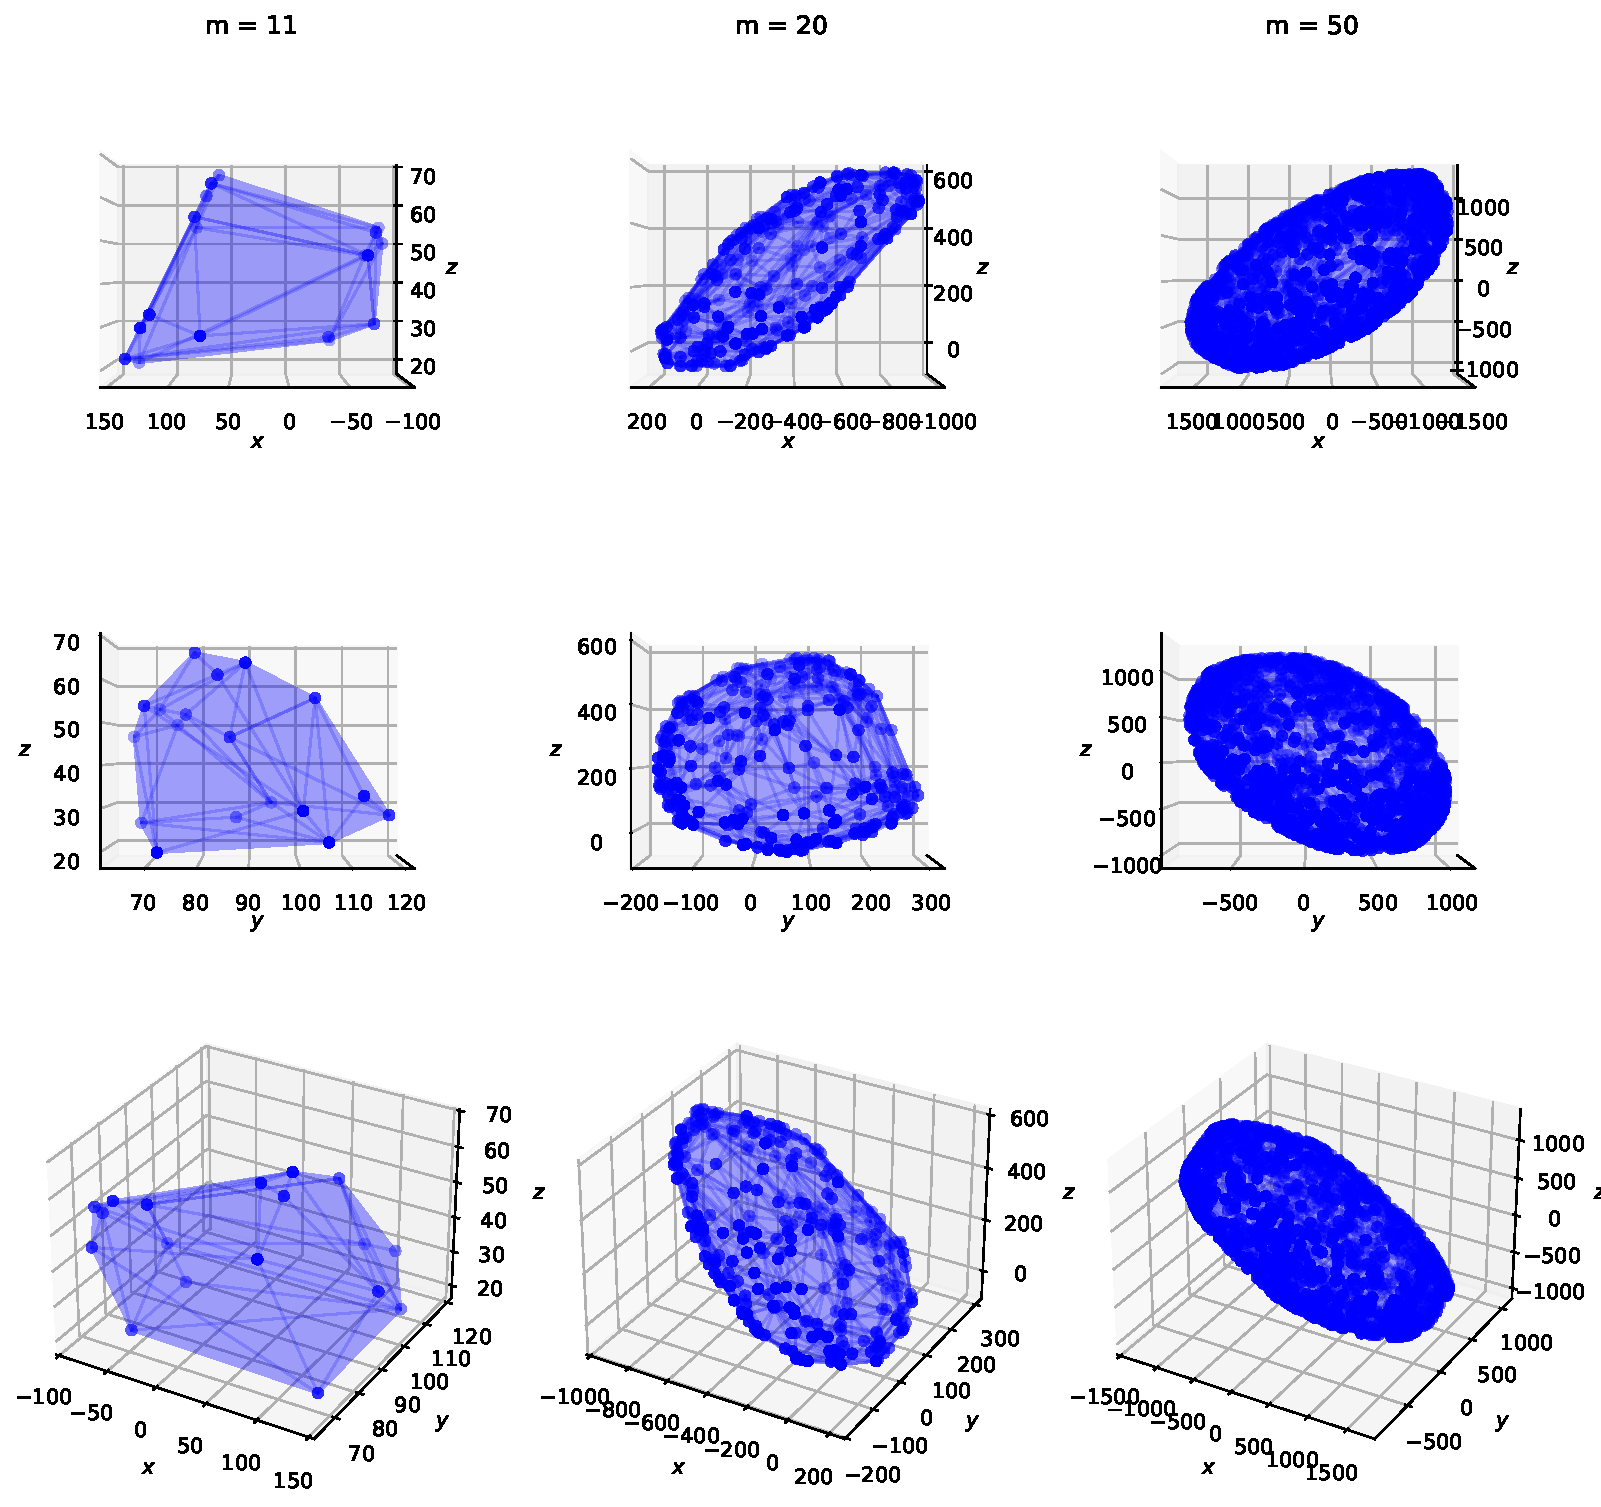
\includegraphics[trim={0 700 0 0},clip, width=0.9\linewidth]{img/chapter_3/zonotopes_looks_like_ellipsoids.pdf}
    \end{minipage}
    \begin{minipage}{1\linewidth}
        \centering
        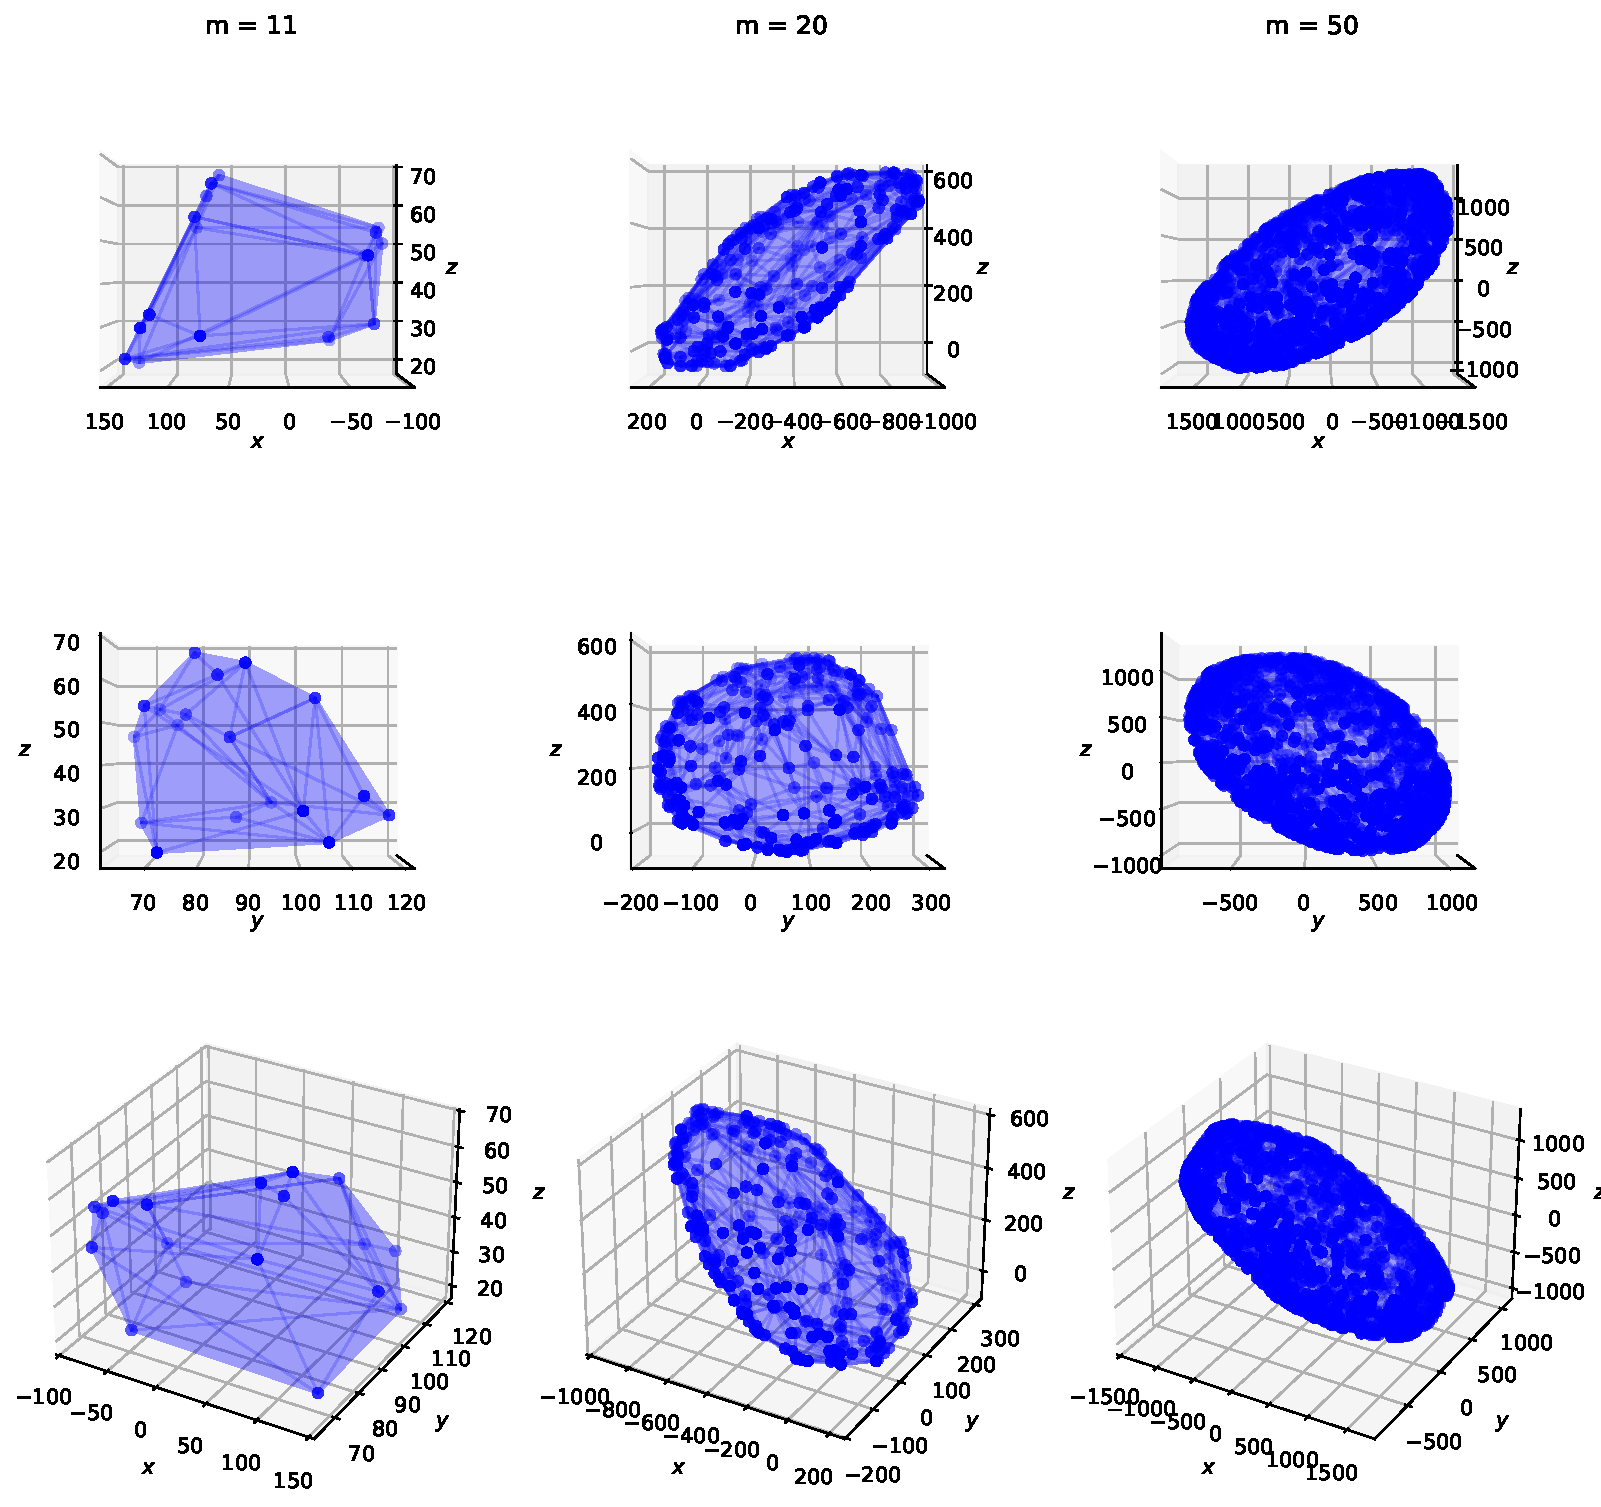
\includegraphics[trim={0 500 0 60},clip, width=0.9\linewidth]{img/chapter_3/zonotopes_looks_like_ellipsoids.pdf}
    \end{minipage}
    \begin{minipage}{1\linewidth}
        \centering
        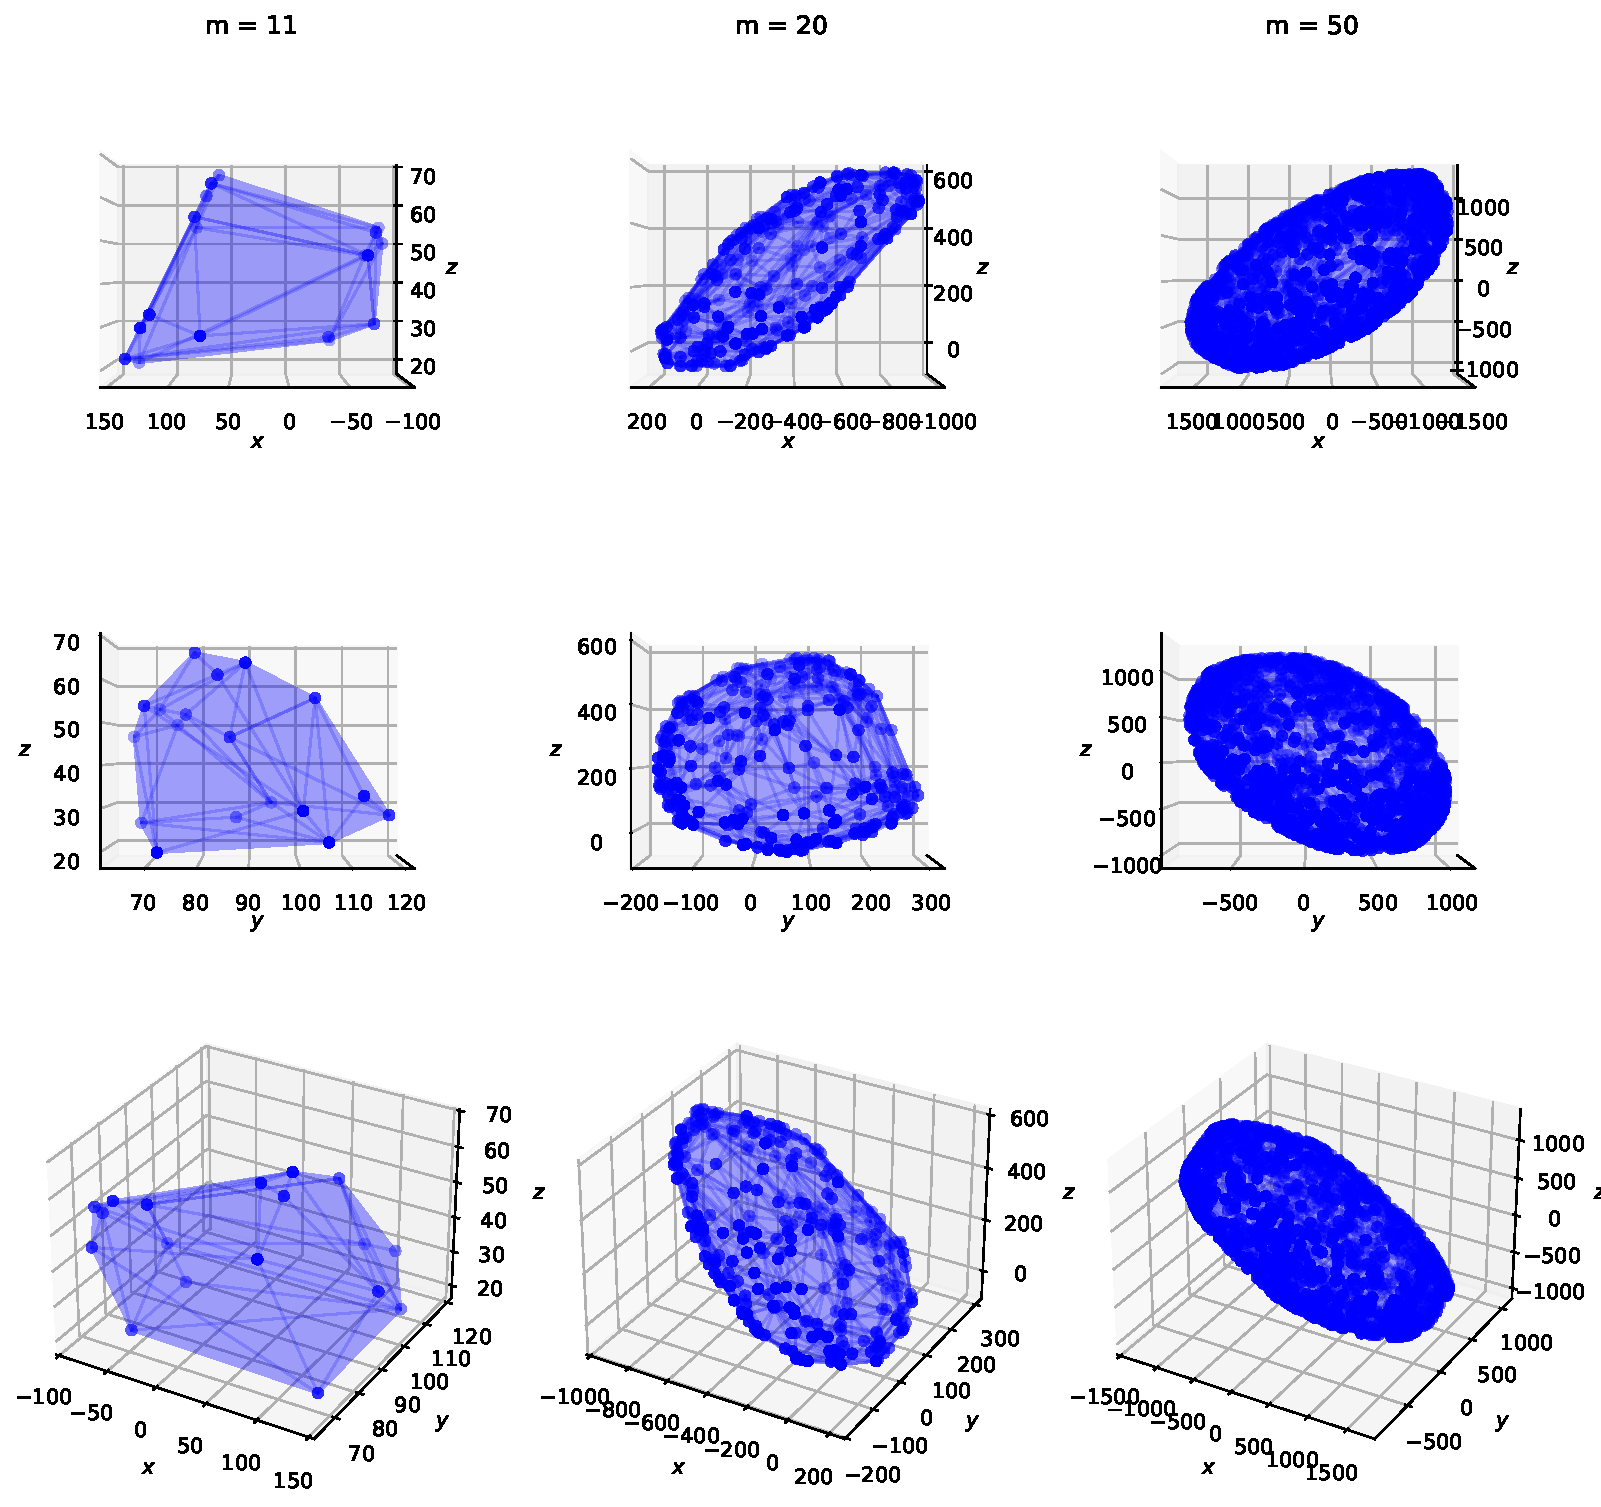
\includegraphics[trim={0 255 0 300},clip, width=0.9\linewidth]{img/chapter_3/zonotopes_looks_like_ellipsoids.pdf}
    \end{minipage}
    \begin{minipage}{1\linewidth}
        \centering
        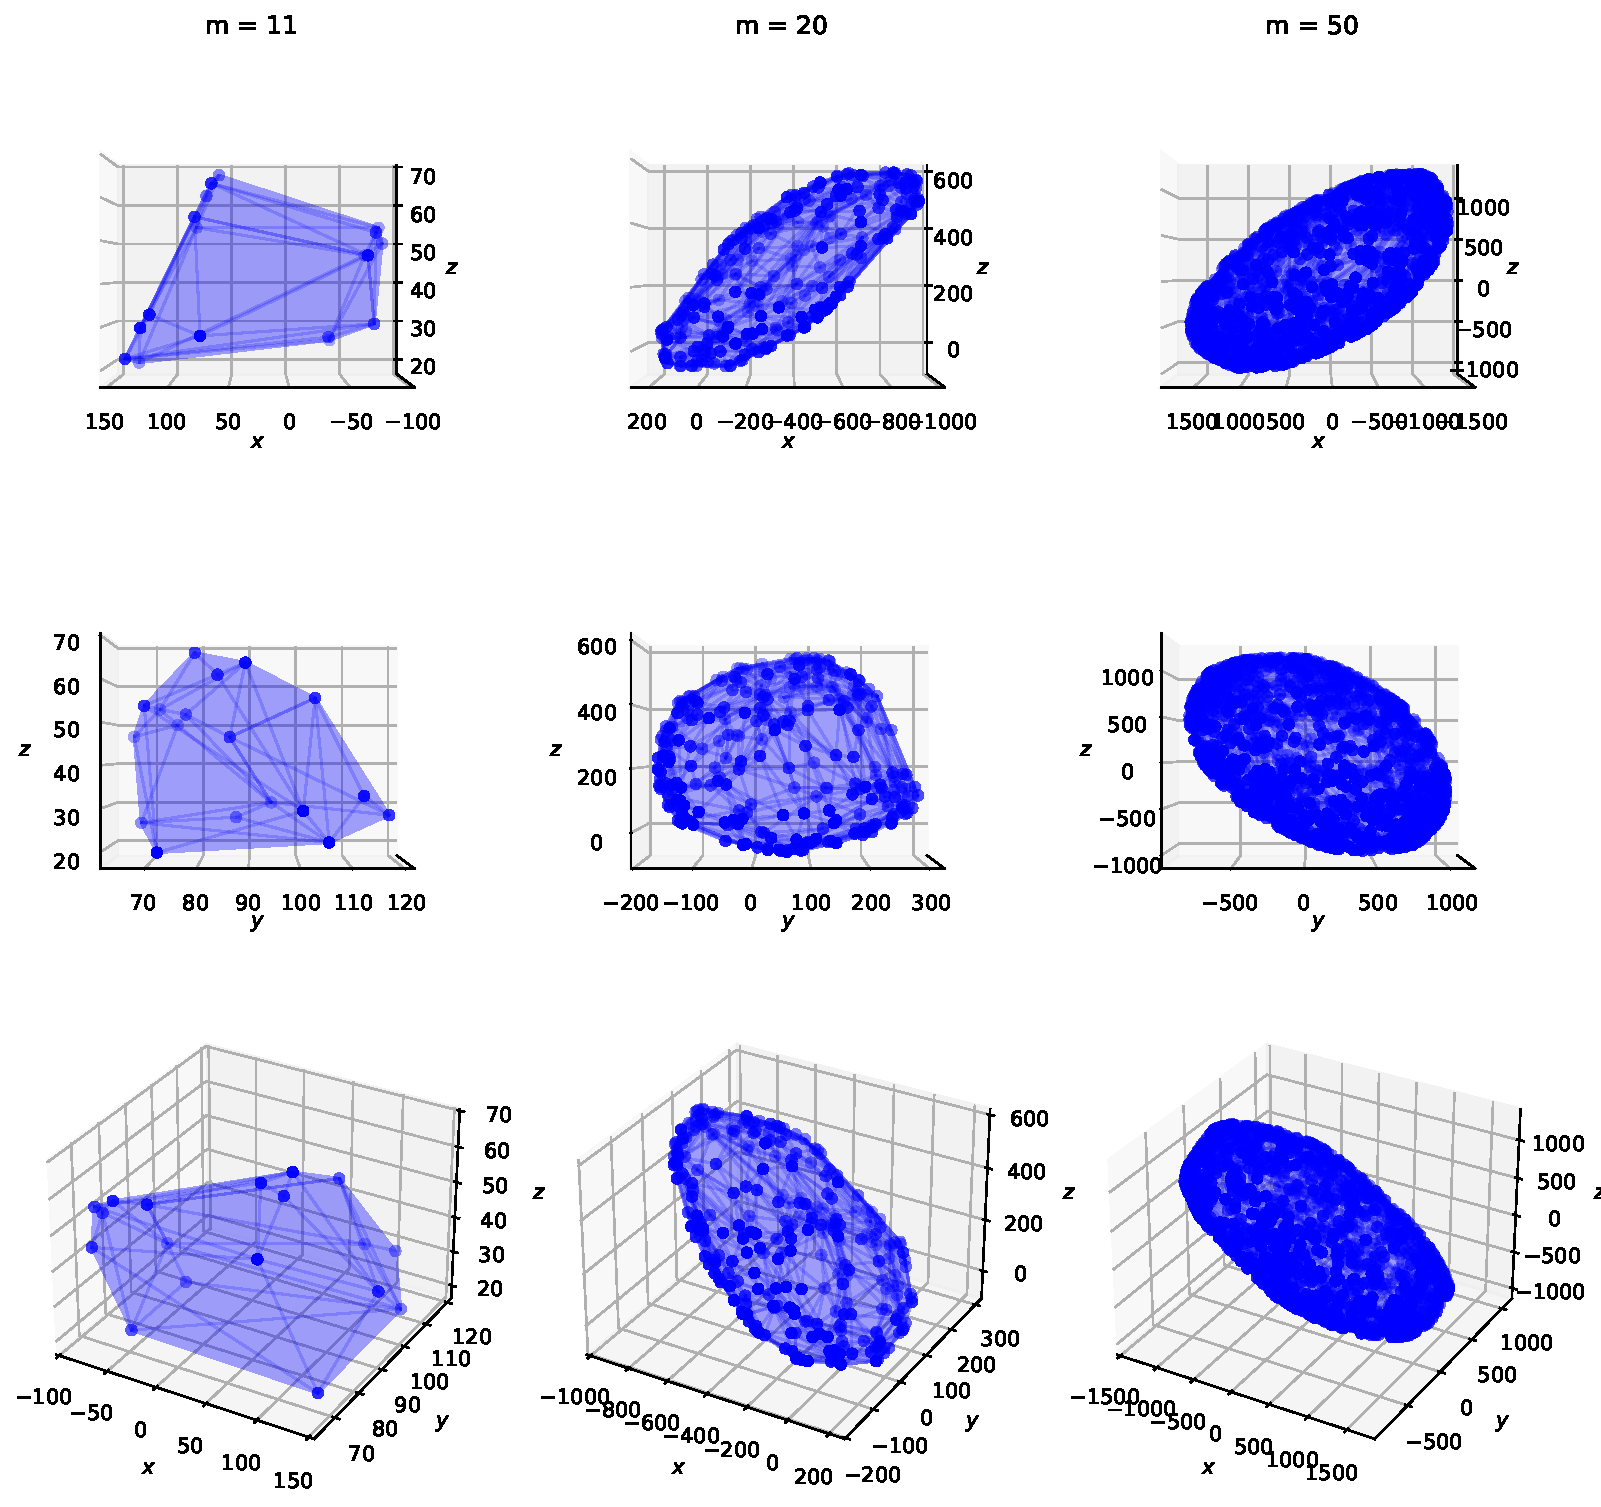
\includegraphics[trim={0 0 0 500},clip, width=0.9\linewidth]{img/chapter_3/zonotopes_looks_like_ellipsoids.pdf}
    \end{minipage}
    
    
    \caption{Each column represents a different number of muscles ($m = 11$, 20, and 50), while each row shows a different orientation of the corresponding force feasible set to provide a better visualization in 3D. As the focus of this section is on the \emph{shape} of the force feasible sets, the axes scales are not uniform across the columns. The lever arm matrix used here is dense (all entries are non-zero), implying that each randomly generated muscle acts on all 7 joint torques.
    }
    \label{fig:example_ellipsoidal_zonotope_multijoints}
\end{figure}

\begin{figure}[!htb]
    \captionsetup{justification=centering}
    \begin{minipage}{1\linewidth}
        \centering
        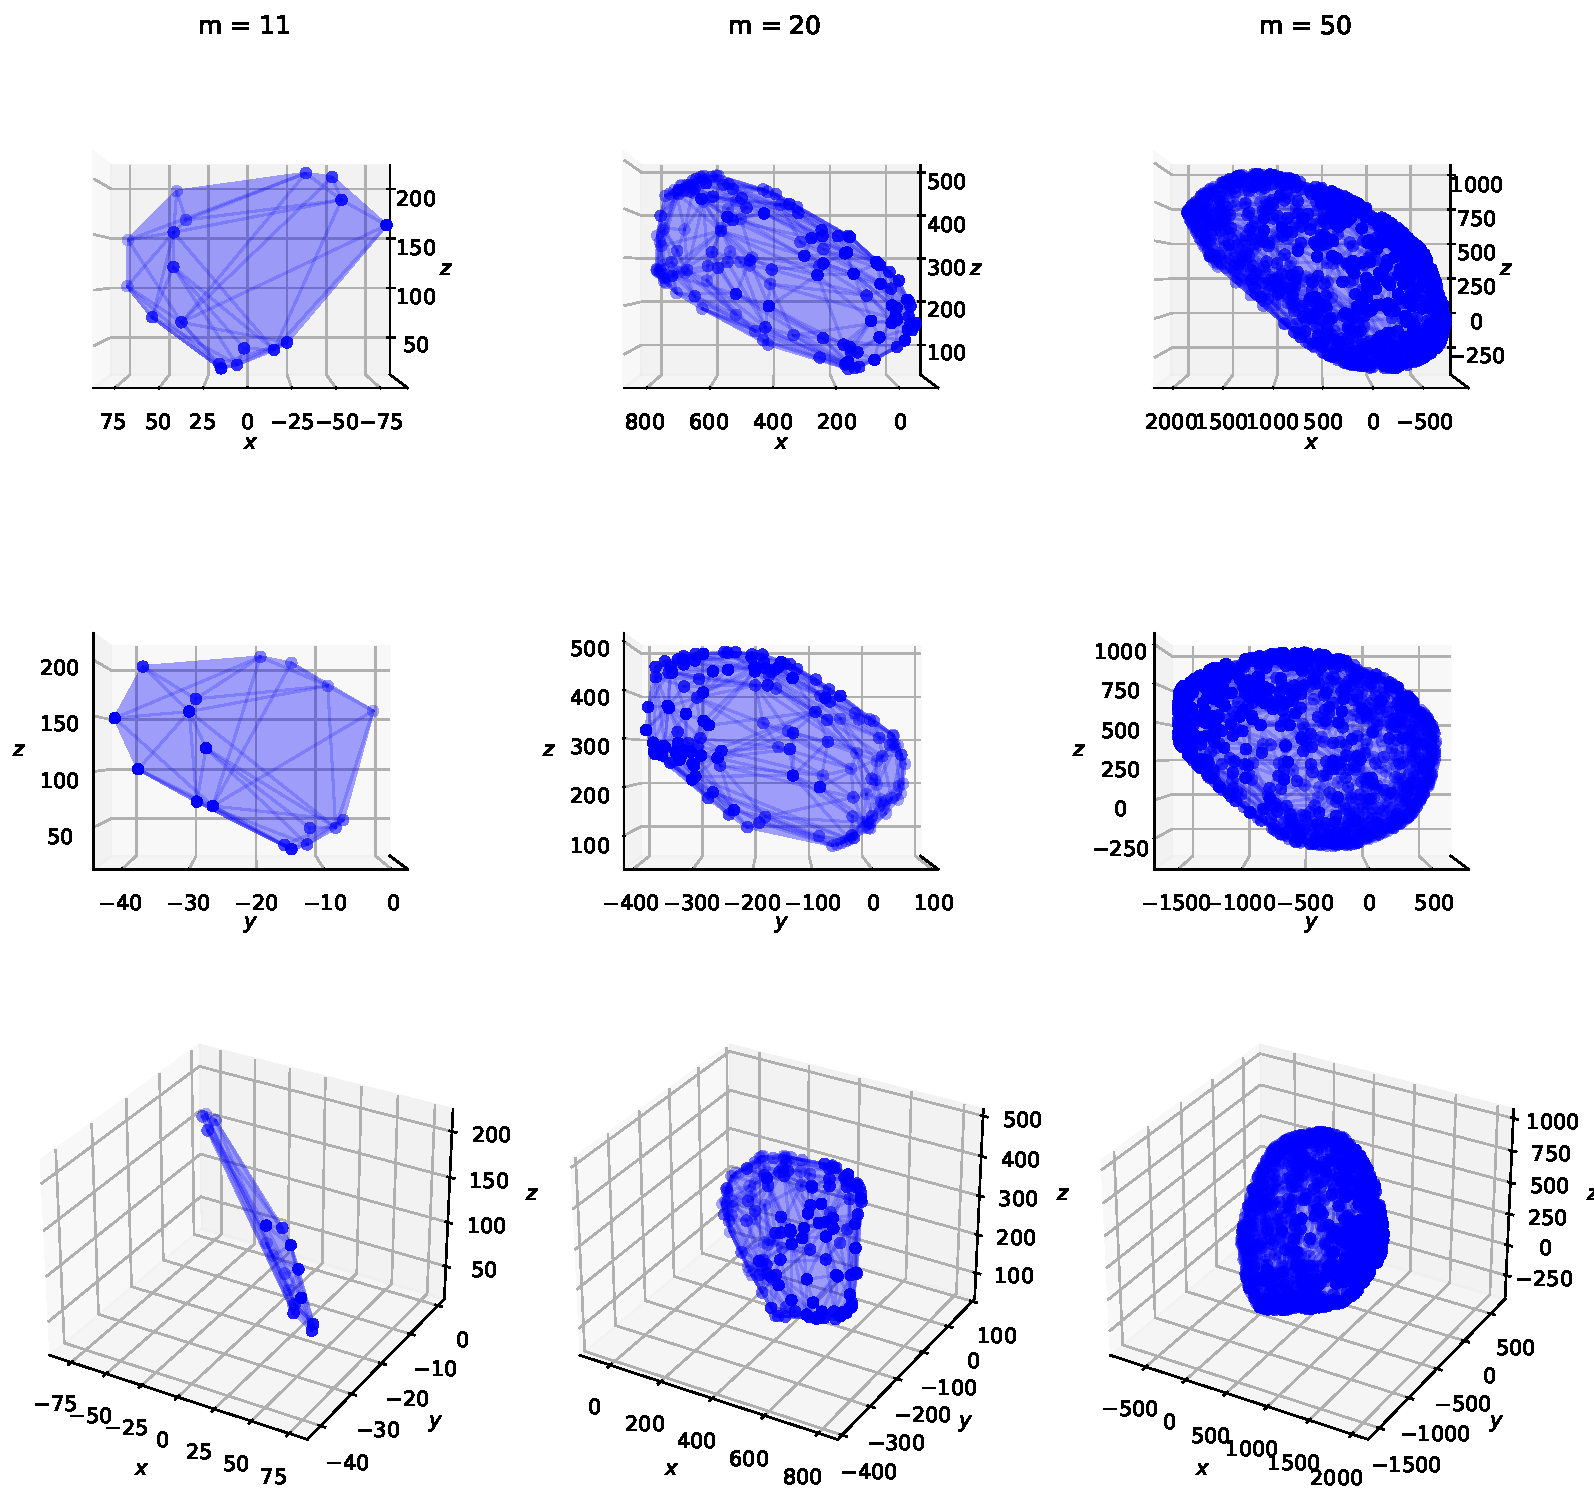
\includegraphics[trim={0 700 0 0},clip, width=0.9\linewidth]{img/chapter_3/zonotopes_looks_like_ellipsoids_2.pdf}
    \end{minipage}
    \begin{minipage}{1\linewidth}
        \centering
        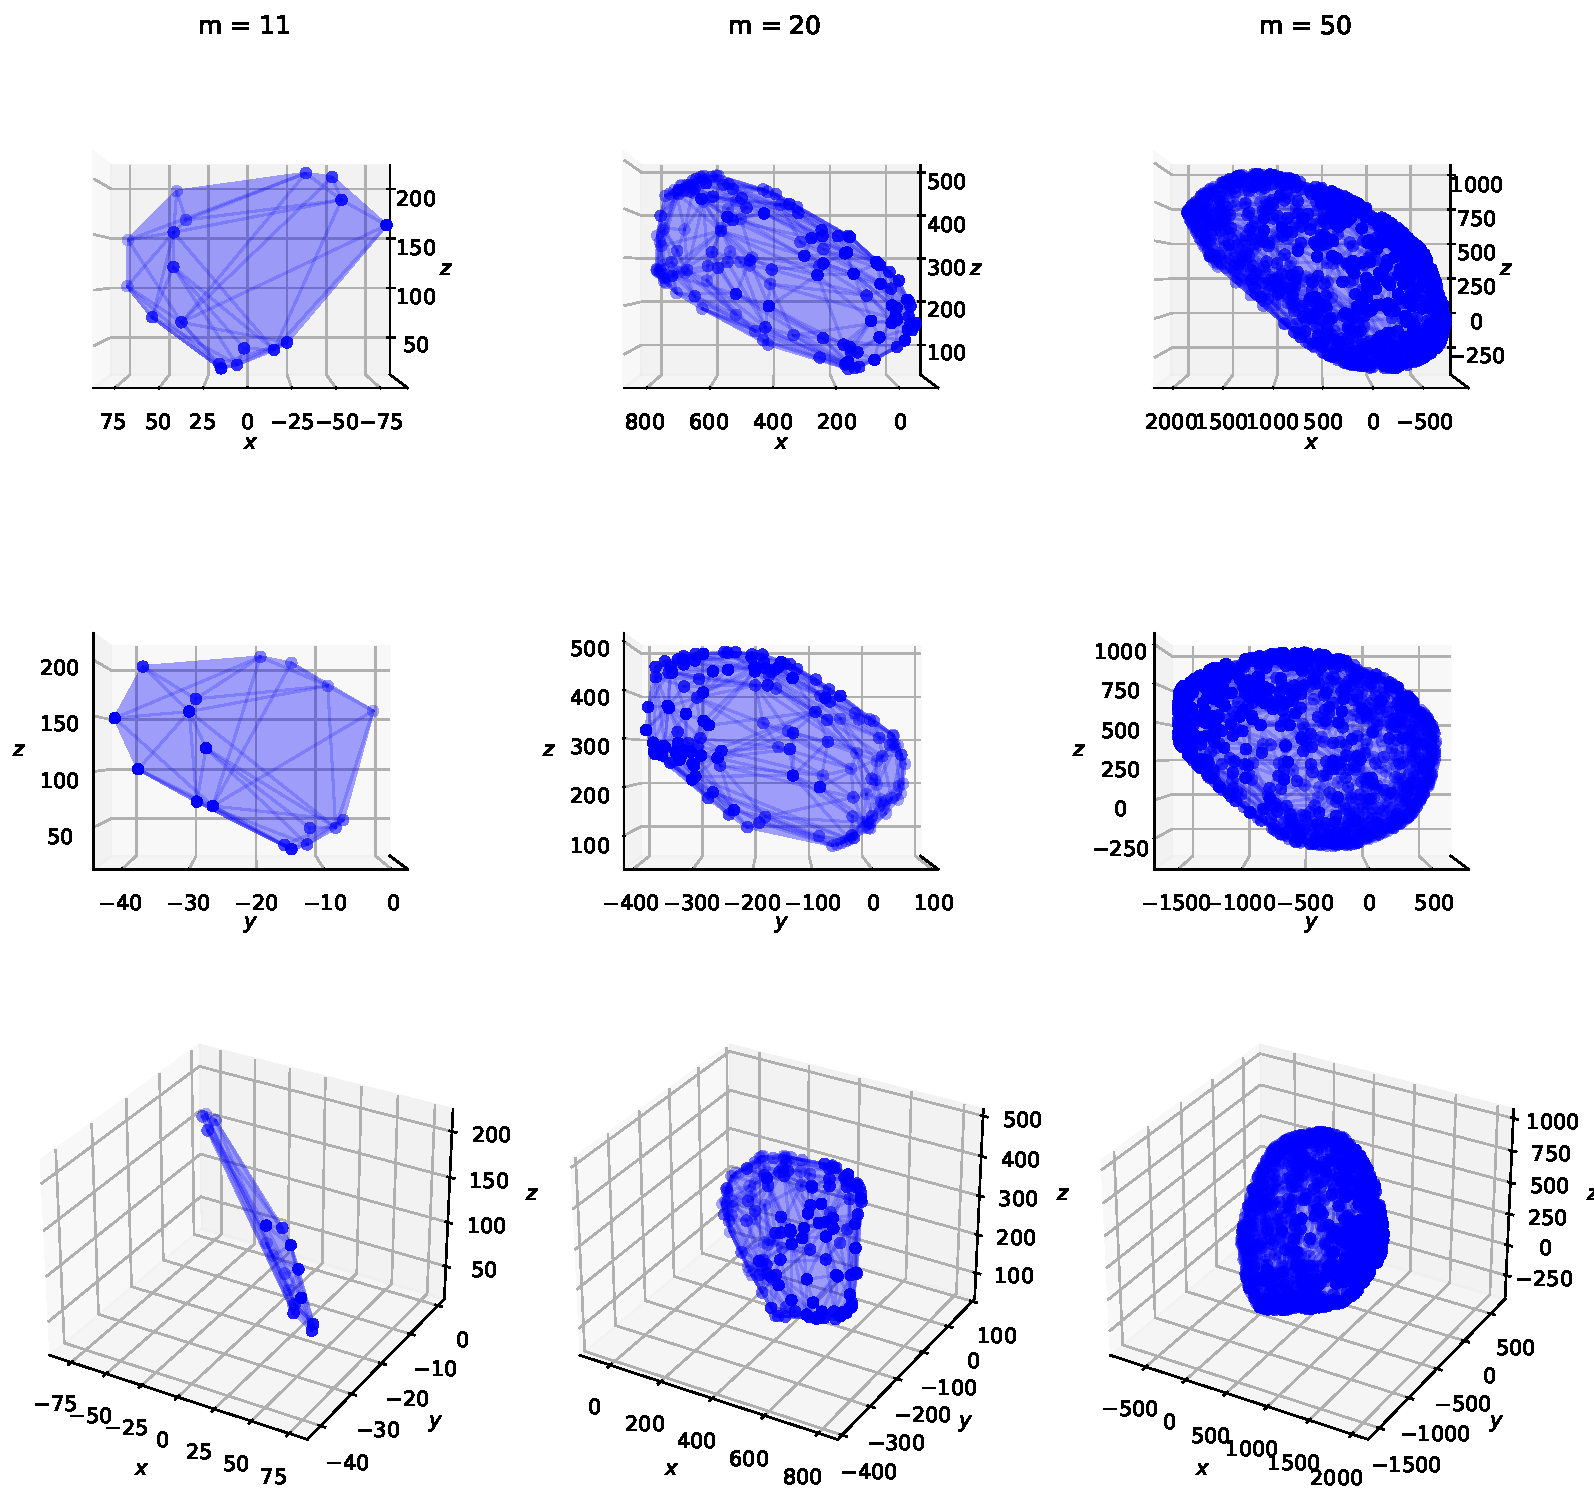
\includegraphics[trim={0 500 0 60},clip, width=0.9\linewidth]{img/chapter_3/zonotopes_looks_like_ellipsoids_2.pdf}
    \end{minipage}
    \begin{minipage}{1\linewidth}
        \centering
        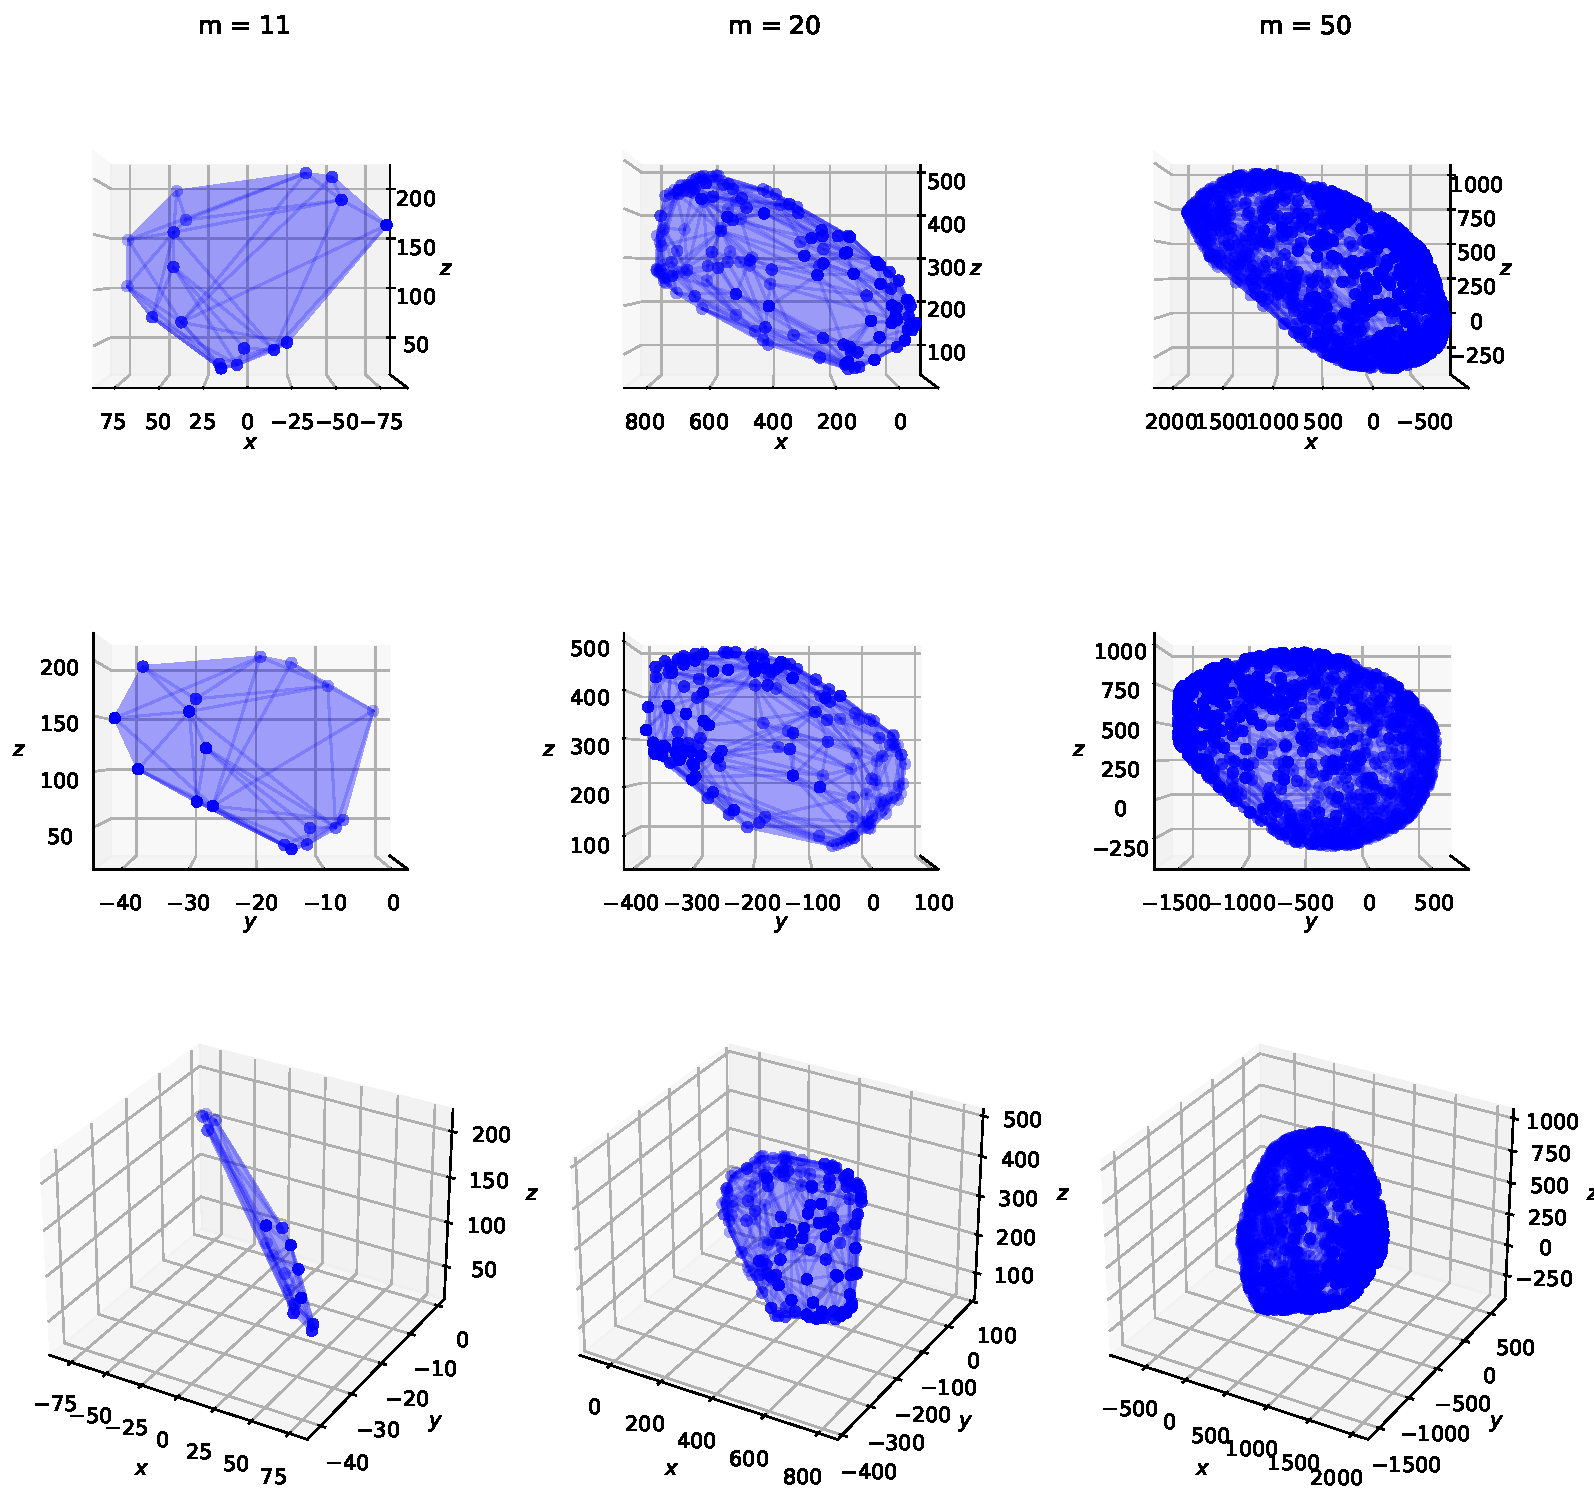
\includegraphics[trim={0 255 0 300},clip, width=0.9\linewidth]{img/chapter_3/zonotopes_looks_like_ellipsoids_2.pdf}
    \end{minipage}
    \begin{minipage}{1\linewidth}
        \centering
        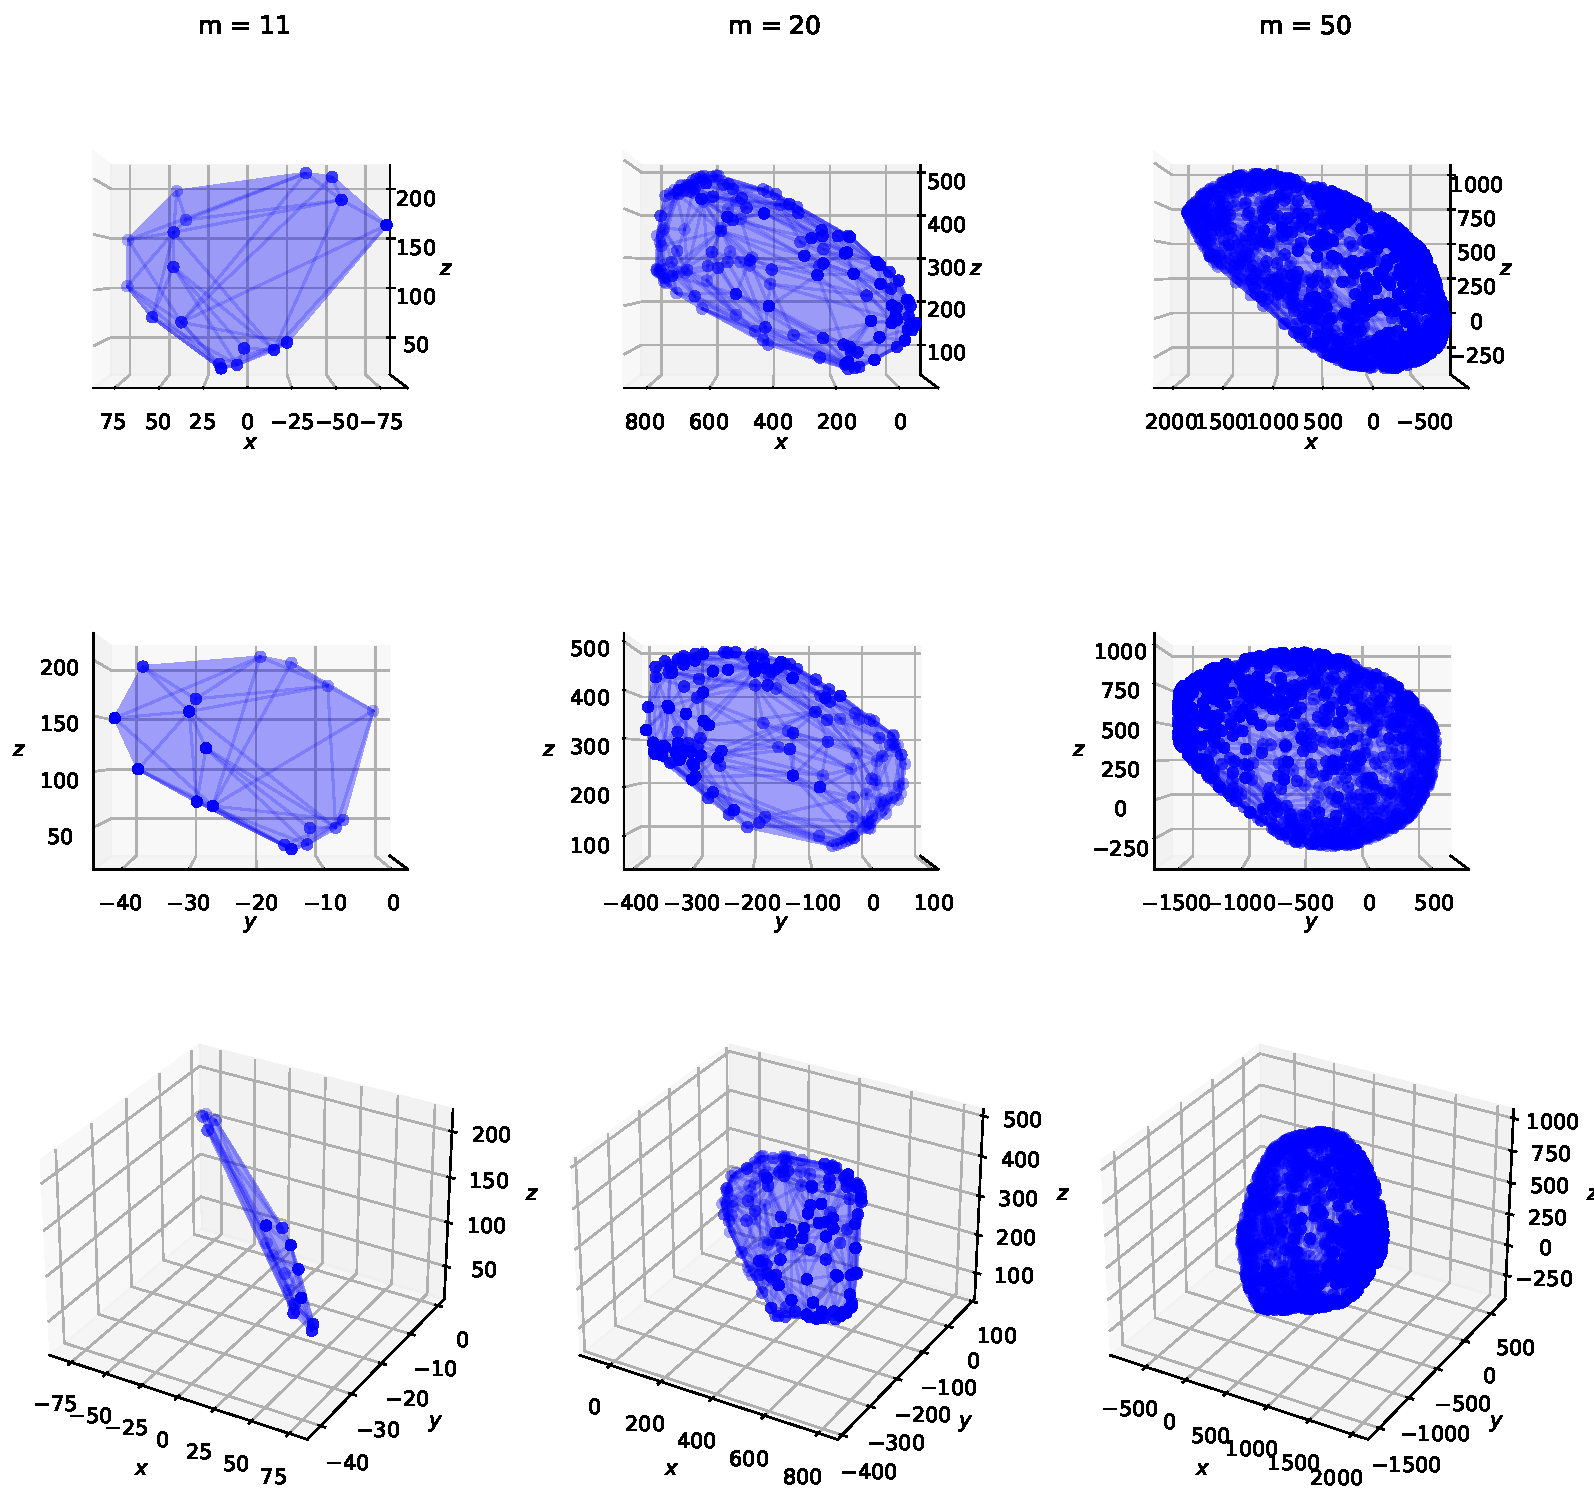
\includegraphics[trim={0 0 0 500},clip, width=0.9\linewidth]{img/chapter_3/zonotopes_looks_like_ellipsoids_2.pdf}
    \end{minipage}
    
    \caption{Each column represents a different number of muscles ($m = 11$, 20, and 50), while each row shows a different orientation of the corresponding force feasible set to aid visualization in 3D. The lever arm matrix used here describes 7 degrees of freedom distributed across two 3D joints and one pin joint, with each muscle acting on at most two joints.}
    \label{fig:example_ellipsoidal_zonotope_bijoints}
\end{figure}

This figure illustrates how the force feasible set can exhibit an ellipsoidal shape. In this example (and indeed in most cases when $-L^T$ is generated as described), the ellipsoidal approximation is qualitatively accurate even with $m = 50$ muscles, which is fewer than the estimated lower bound of $m \geq 68$. This observation can be attributed to the geometric construction underlying Milman's Quotient of Subspace Theorem (Theorem \ref{th:milman_quotient_subspace_theorem}). Notably, this ellipsoidal shape emerges even when considering a non-zero gravitational vector and a non-centered tension cube, conditions that were not explicitly addressed in Milman's theorem, though they were hypothesized.

However, in a realistic biomechanical context, muscles typically do not act on all joints.  Muscles can be mono-articular (acting on a single joint) or bi-articular (acting on two joints). In Figure \ref{fig:example_ellipsoidal_zonotope_bijoints}, we resampled $-L^T$ to reflect this: the 7 rows of $-L^T$ are divided into 3 groups, representing three joints. The first group corresponds to the first 3 rows, the second to rows 4 to 6, and the third to the last row (which could represent a pin joint).  A muscle is said to \emph{act} on a joint if the corresponding entries in its column in $-L^T$ are non-zero.

In this resampled model, the first 15 muscles act on the first joint only, the next 5 on the first and second joints, the next 15 on the second joint only, the next 10 on the second and third joints, and the final 5 on the third joint. While these choices are arbitrary, they reflect the prevalence of mono- and bi-articular muscles in biological systems. The results are depicted in Figure \ref{fig:example_ellipsoidal_zonotope_bijoints}, where an ellipsoidal shape emerges even with just 20 muscles.

\subsection*{Conclusion}
One of the goals of this thesis is to understand the shape of the force feasible set and how it reflects muscle properties. In the literature, such a set can be represented as either a polytope or an ellipsoid, implying that the underlying tension feasible set is modeled as a cube or a sphere, respectively.  However, we have argued that, regardless of how the tension feasible set is modeled (it shall however be convex), the force and torque feasible sets tend to resemble ellipsoids when a sufficiently large number of muscles are considered. This property stems from their inherent geometric construction.

Despite this tendency towards an ellipsoidal shape, there are significant differences in \emph{size} between different tension feasible set models. One way to account for these size variations is to directly compute an ellipsoidal approximation of the force feasible set derived from a $\mathcal{T}_{\infty}$ model.

Let us explore some common ellipsoidal approximations and discuss their computational limitations. The \emph{inner and outer Löwner-John ellipsoids} are often used to approximate convex bodies. For an $n$-dimensional convex set $C$, its inner ellipsoid (or John ellipsoid) is the $n$-dimensional ellipsoid of maximal volume inscribed in $C$, while its outer ellipsoid (or Löwner ellipsoid) is the circumscribed ellipsoid of minimal volume.  A key result establishes the uniqueness of both the inner and outer ellipsoids for a given convex set (\cite{henkLownerJohnEllipsoids2012}). However, as noted in (\cite{cernyGoffinAlgorithmZonotopes2012}), Löwner-John ellipsoids cannot be computed algorithmically in general, necessitating approximation methods.

In our context, we collect measurements of maximal exerted forces, represented as points in Cartesian space. The inner ellipsoid can be constructed from a set of bounding hyperplanes, while the outer ellipsoid can be constructed from a set of points.  While constructing these ellipsoids for a set of experimental forces is feasible, attempting to fit a musculoskeletal model that reproduces the experimental ellipsoid is computationally intractable. This would require computing the vertices of the torque zonotope (and transforming them into hyperplane inequalities) before computing the inner or outer ellipsoid. Due to the combinatorial complexity of enumerating these vertices (see Chapter \ref{chapter:2}), this approach is not viable.

Another challenge arises when the tension feasible set $\mathcal{T}$ is derived from a $p$-ball. When projected onto the torque space, except for the cases $p = 1$, 2, or $\infty$, there is no explicit description of the surface of the resulting convex set. While sampling methods could be employed, for a large number of muscles, the sampling of the unit $p$-ball would require a vast number of points, and the probability of sampling an extremal point of $\mathcal{T}$ that projects onto an extremal point of the torque feasible set is effectively zero.

Instead of directly computing ellipsoidal approximations from a set of points, we aim to gain a deeper understanding of how the shape and dimension of the tension feasible set influence the size of the torque and force feasible sets. The next section, while initially theoretical, introduces a computational tool that provides a simple formula for approximating the force feasible set with an ellipsoid when a large number of muscles are involved. This formula does not require computing any points, thus circumventing the combinatorial challenges associated with enumerating zonotope vertices. Moreover, it extends to all $\mathcal{T}_p$ models.

\section{Accounting for the projected volume problem}
\label{sec:projected_volume_problem}
Our primary objective in this section is to demonstrate that when a large number of muscles are considered, the choice of a tension feasible set $\mathcal{T}_p$ modeled as a unit $p$-ball primarily affects the volume of the resulting force feasible set, with minimal impact on its shape. We focus on the inherent volume changes that occur when projecting convex sets onto lower-dimensional spaces. Subsection \ref{subsec:proj_unit_p_ball} illustrates this phenomenon through examples, while Subsection \ref{subsec:projection_constant} delves into the underlying mechanisms.  Leveraging the concept of \emph{projection constants} from Banach space theory, we introduce a powerful computational tool to address these volume changes and provide guidance on the choice of a suitable $p$-norm.

\subsection{Projection of unit \emph{p}-balls}
\label{subsec:proj_unit_p_ball}
As an introductory example, consider the force polytopes depicted in Figure \ref{fig:example_ellipsoidal_zonotope_bijoints}. In that figure, different scales were used to emphasize the shapes of the polytopes rather than their sizes.  Figure \ref{fig:example_ellipsoidal_zonotope_bijoints_same_scale} displays the same polytopes using a uniform scale to highlight the differences in their volumes.

\begin{figure}[!htb]
    \captionsetup{justification=centering}
    \begin{minipage}{1\linewidth}
        \centering
        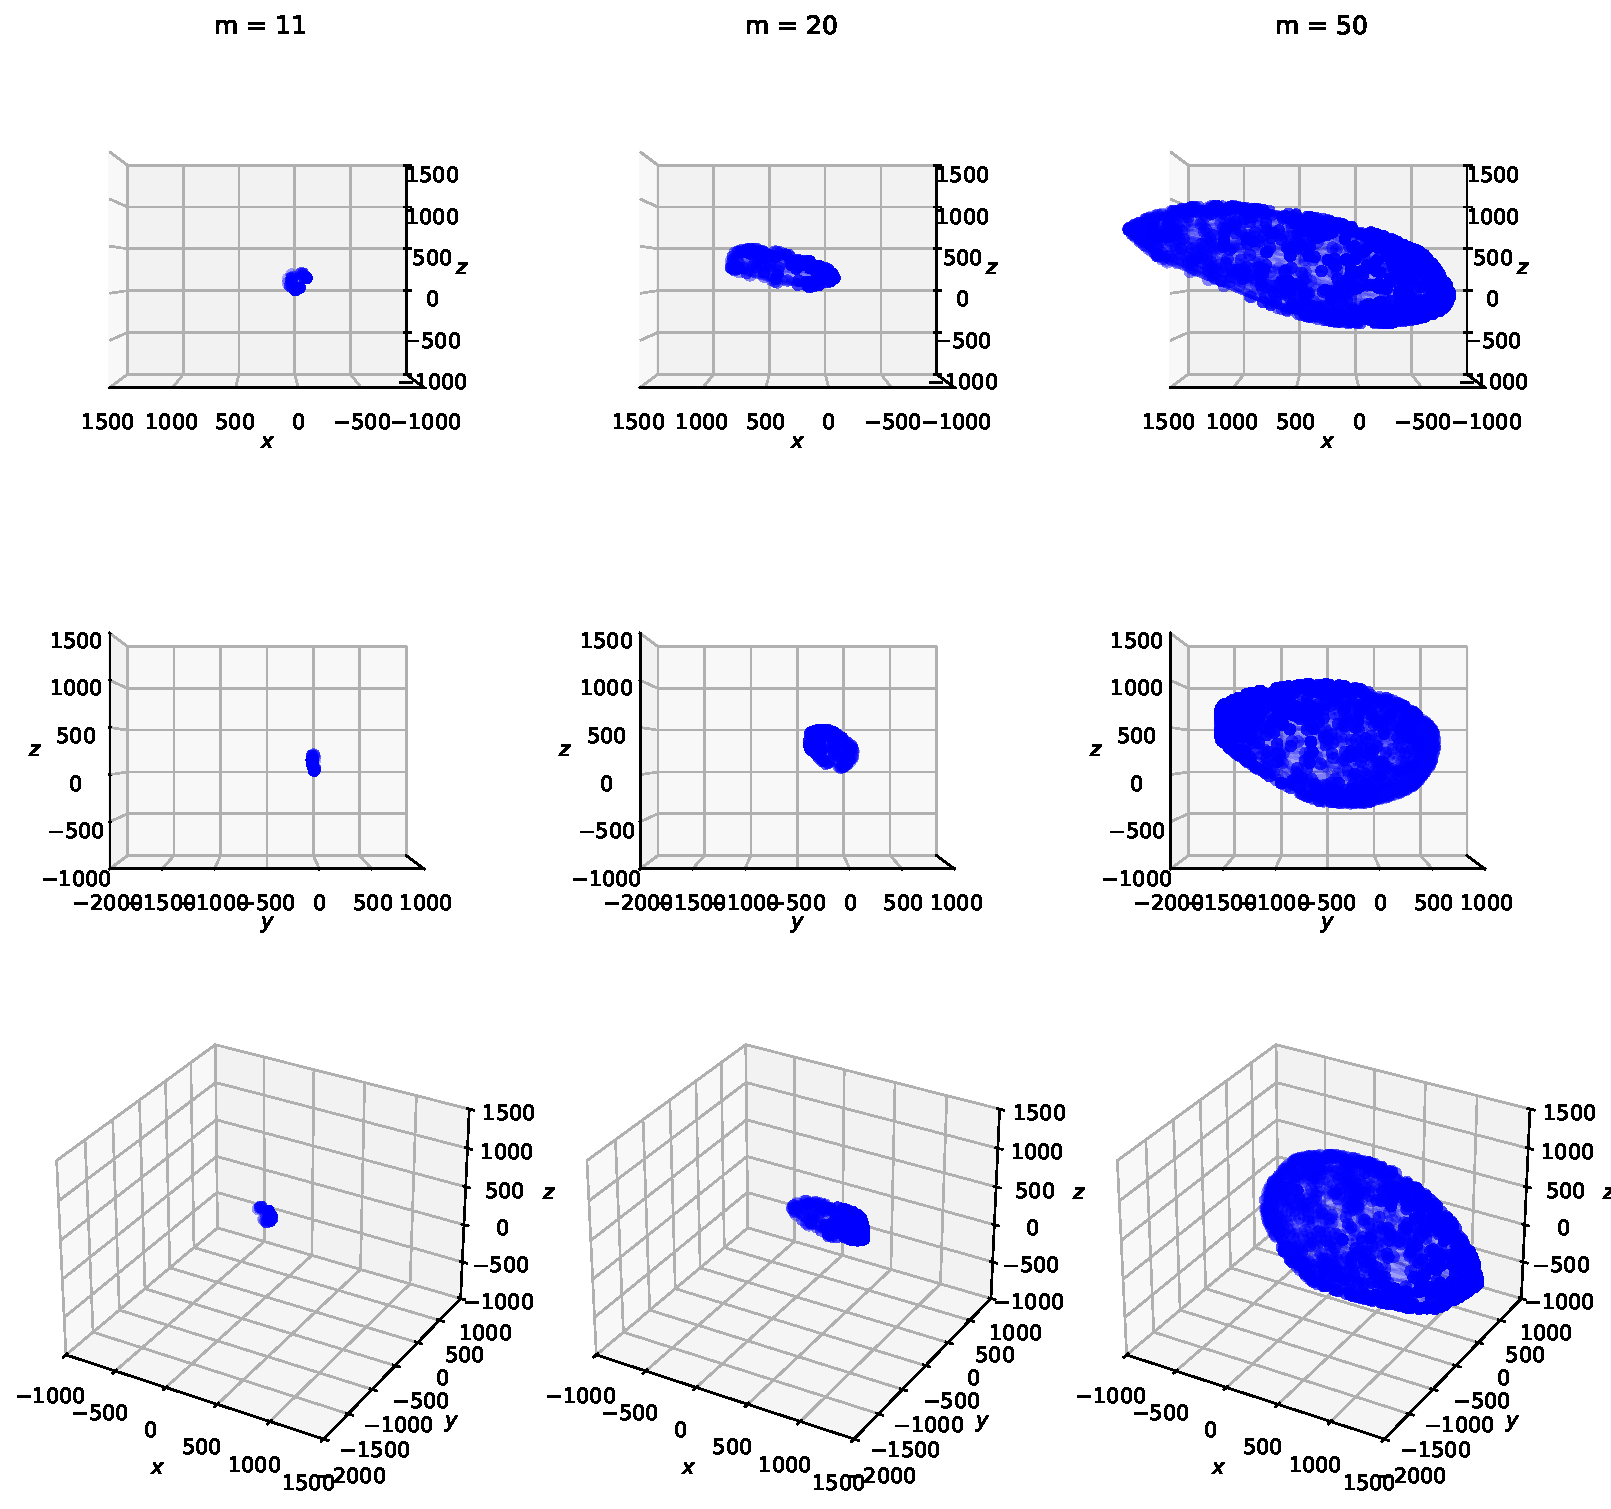
\includegraphics[trim={0 700 0 0},clip, width=0.9\linewidth]{img/chapter_3/zonotopes_looks_like_ellipsoids_2_same_scale.pdf}
    \end{minipage}
    \begin{minipage}{1\linewidth}
        \centering
        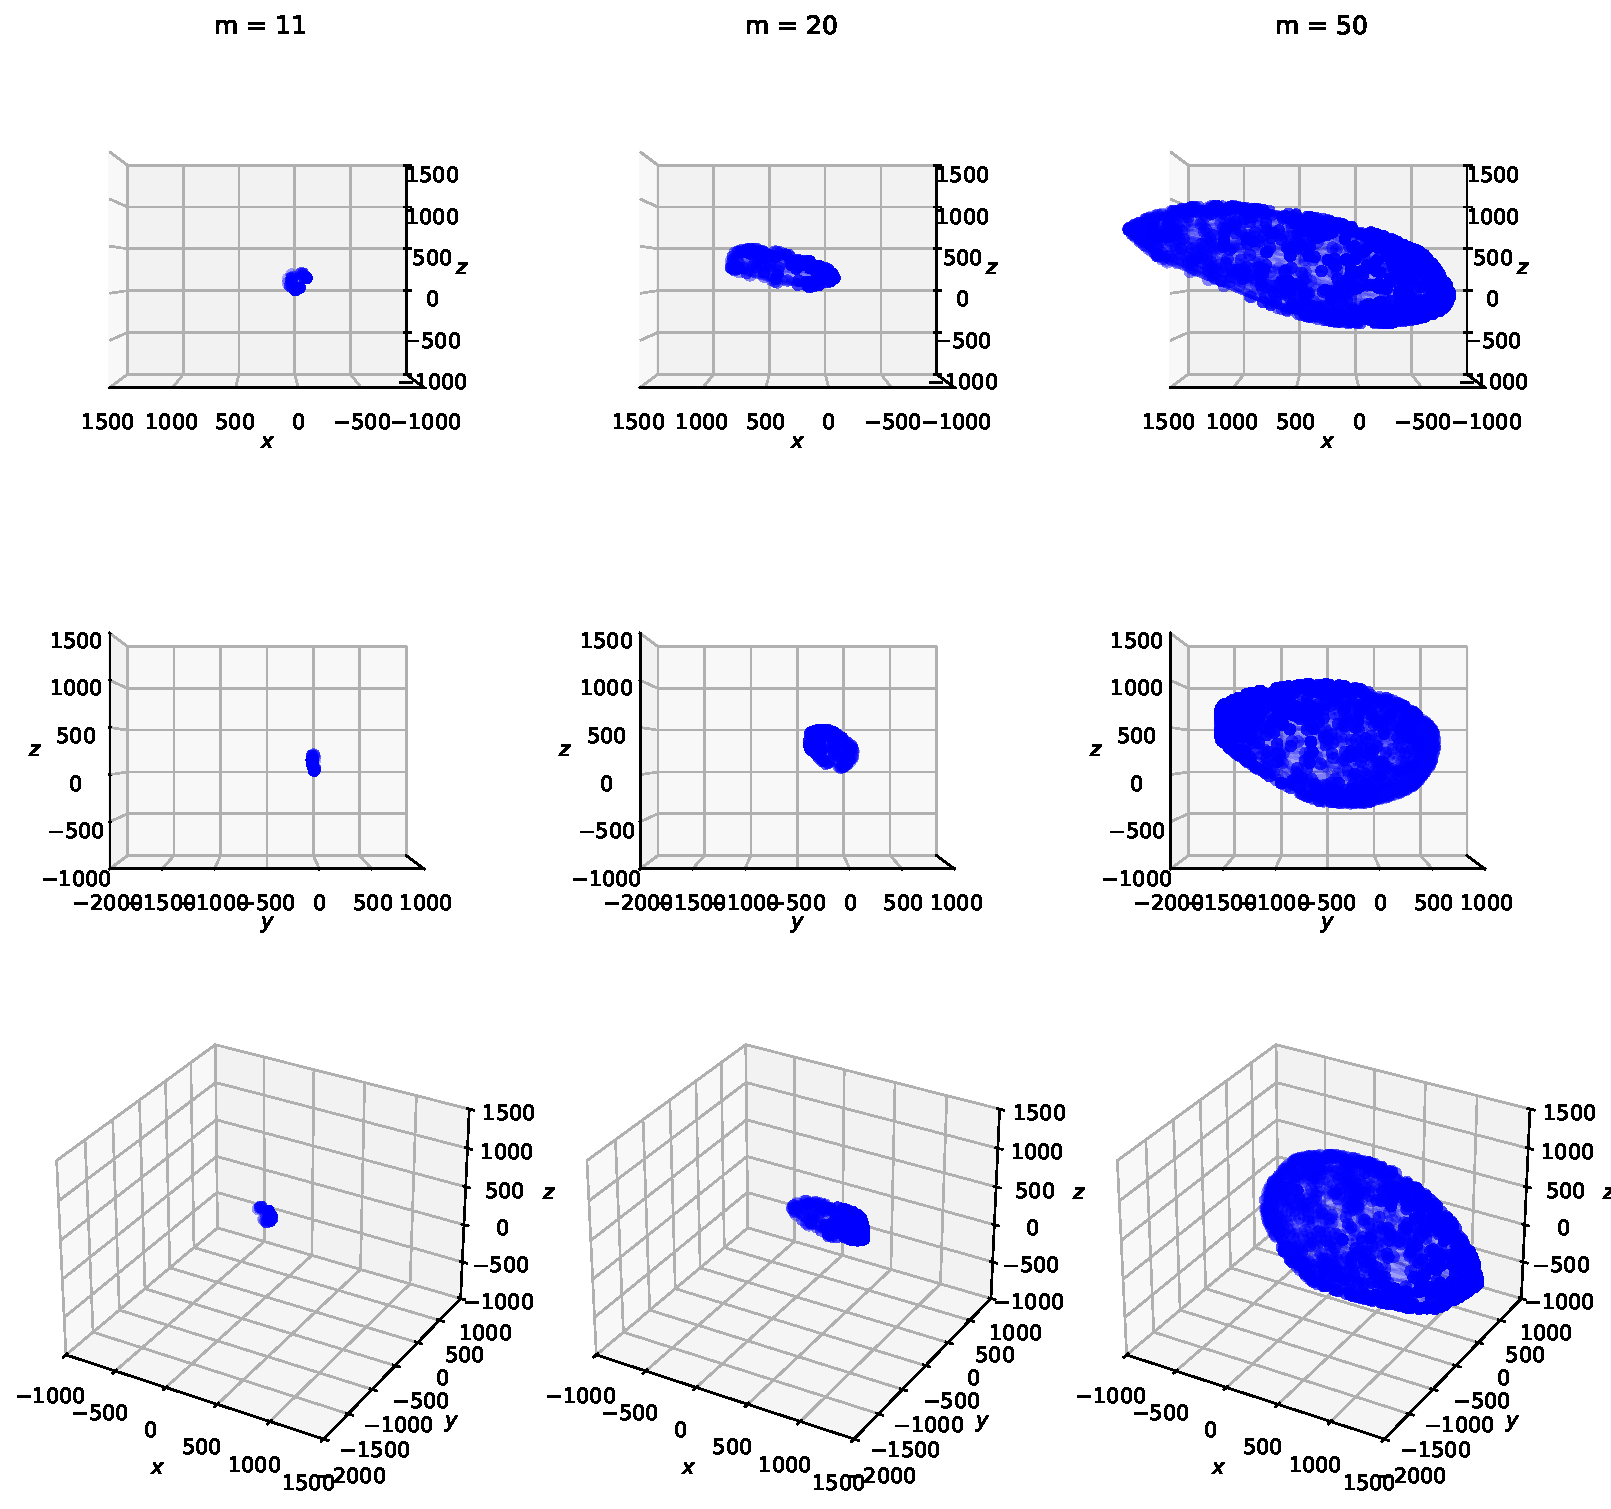
\includegraphics[trim={0 500 0 60},clip, width=0.9\linewidth]{img/chapter_3/zonotopes_looks_like_ellipsoids_2_same_scale.pdf}
    \end{minipage}
    \begin{minipage}{1\linewidth}
        \centering
        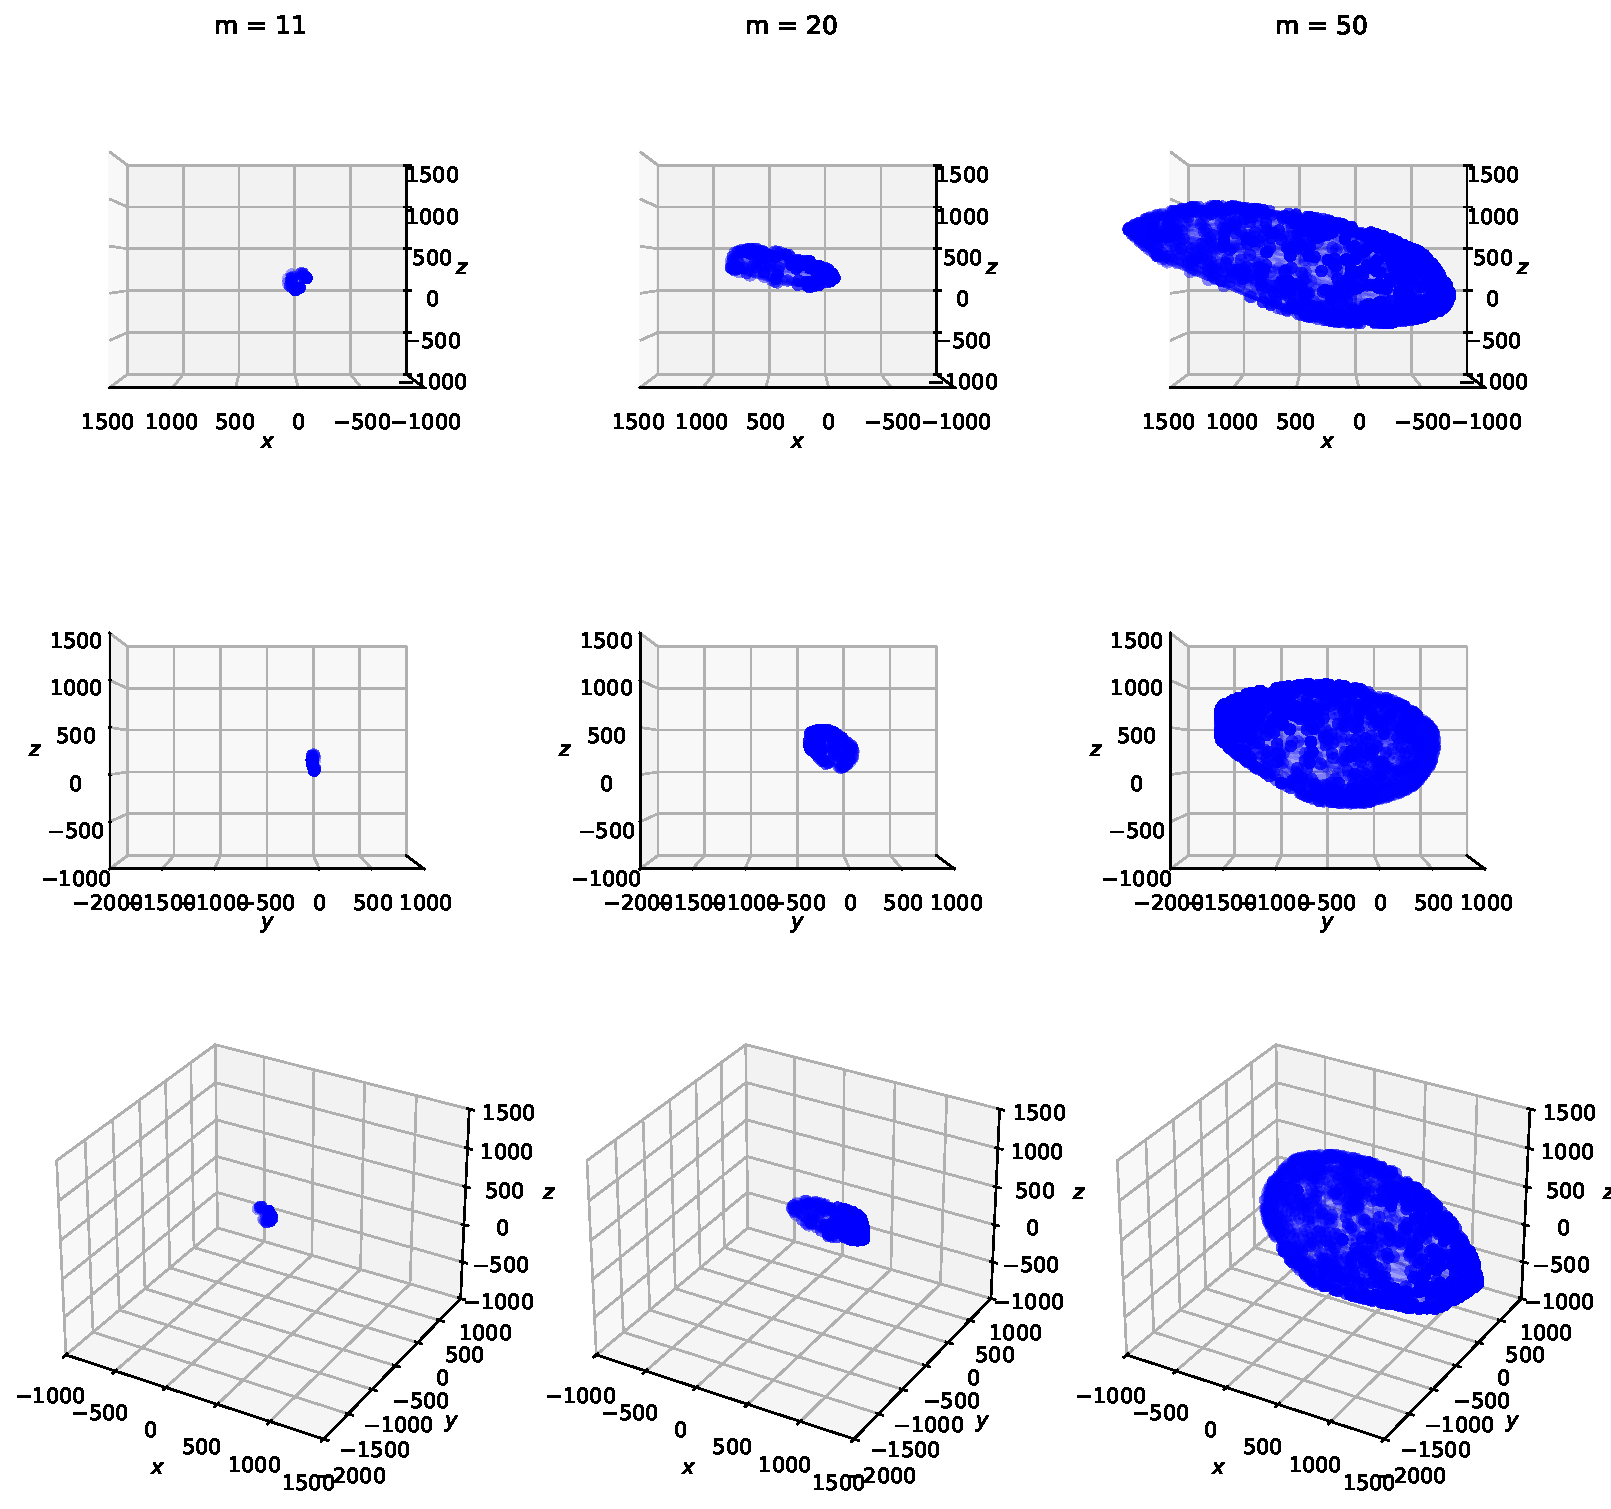
\includegraphics[trim={0 255 0 300},clip, width=0.9\linewidth]{img/chapter_3/zonotopes_looks_like_ellipsoids_2_same_scale.pdf}
    \end{minipage}
    \begin{minipage}{1\linewidth}
        \centering
        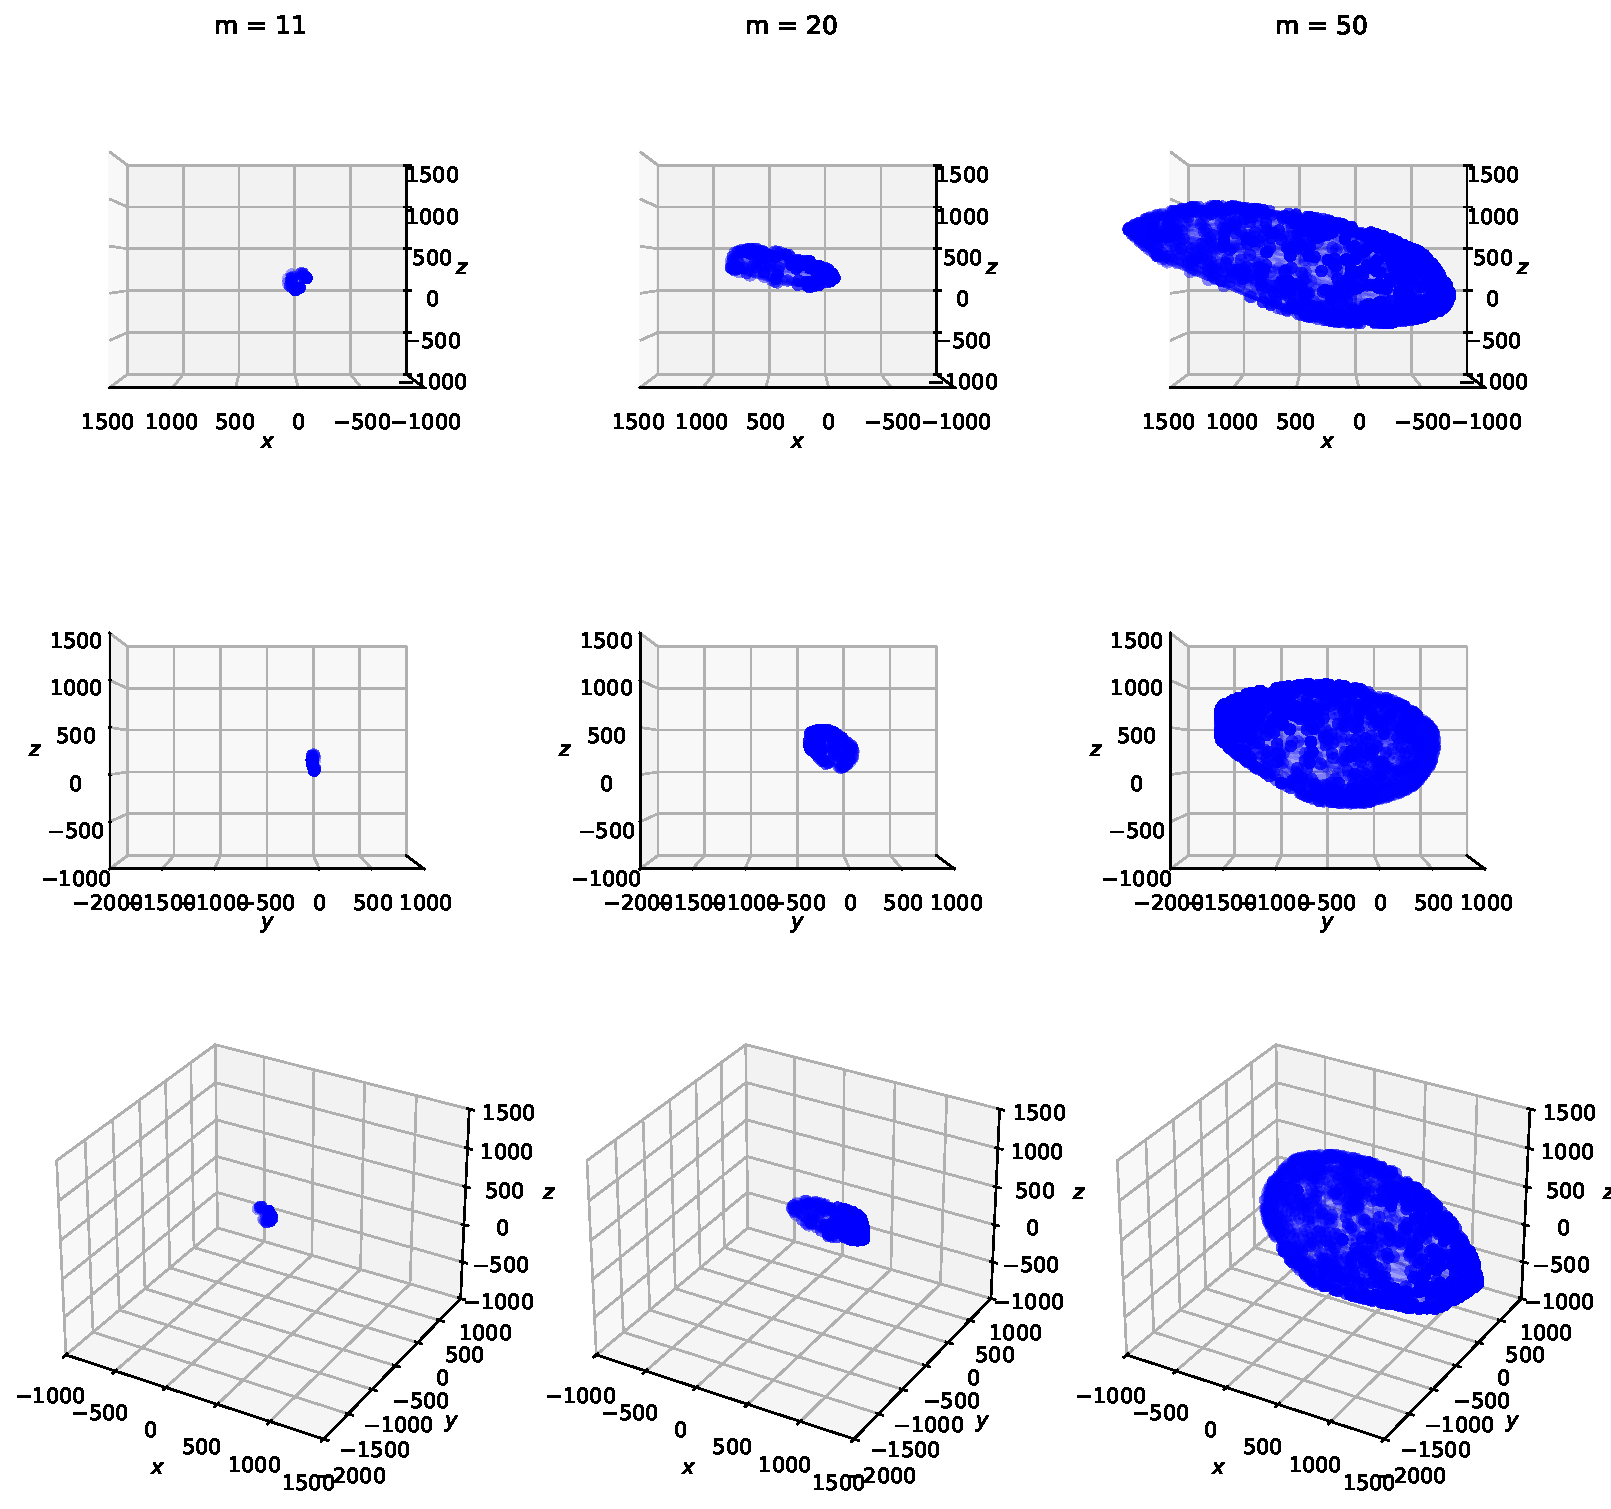
\includegraphics[trim={0 0 0 500},clip, width=0.9\linewidth]{img/chapter_3/zonotopes_looks_like_ellipsoids_2_same_scale.pdf}
    \end{minipage}
    
    \caption{Force feasible sets computed with the same parameters as in Figure \ref{fig:example_ellipsoidal_zonotope_bijoints}, but displayed using a uniform scale to highlight the differences in their volumes.}
    \label{fig:example_ellipsoidal_zonotope_bijoints_same_scale}
\end{figure}

A key observation from the previous figures is that the volume of the force feasible set appears to increase with the number of muscles.  Since we used a cube for the tension feasible set, this can be attributed to the Minkowski sum operations involved in projecting the cube to create the torque feasible set - which is a zonotope.  If a sphere were used instead of a cube, the resulting force ellipsoids would exhibit a less pronounced increase in volume. This is illustrated in Figure \ref{fig:ellipsoid_scale}.
\begin{figure}[!htb]
  \captionsetup{justification=centering}
  \begin{minipage}{1\linewidth}
    \centering
    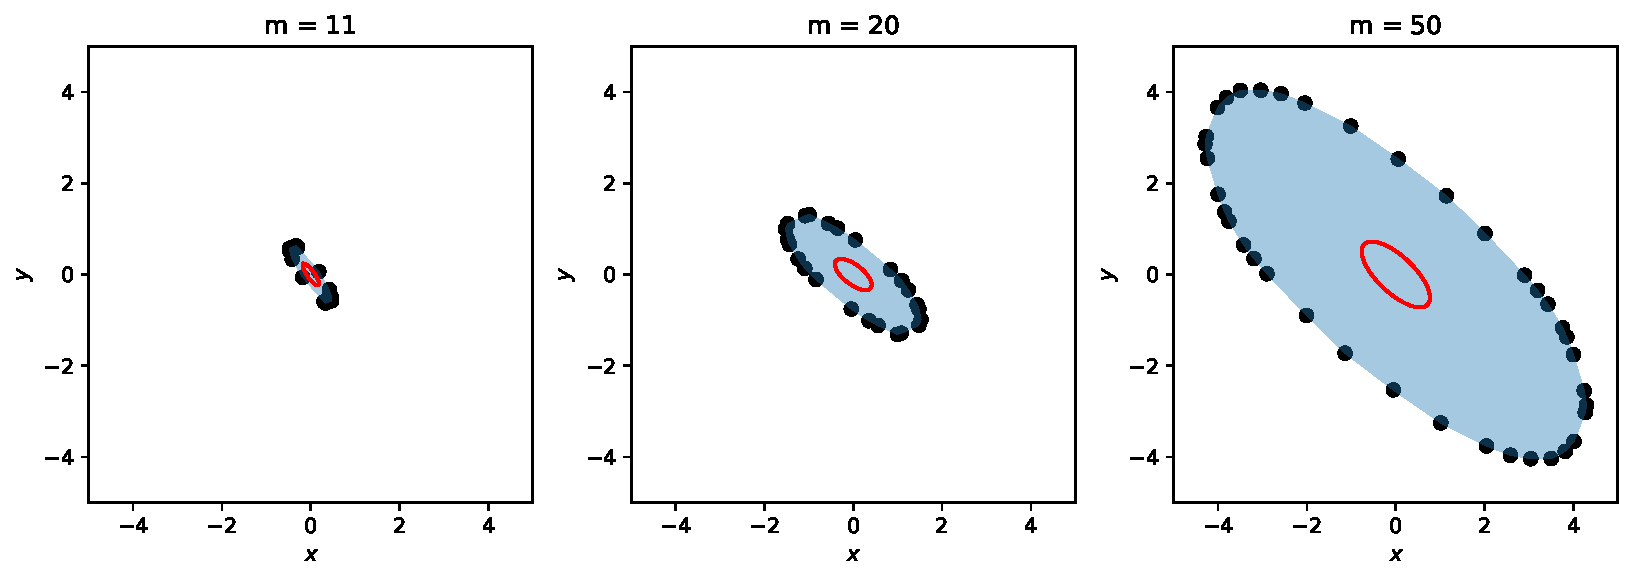
\includegraphics[trim={0 261 0 0},clip, width=0.9\linewidth]{img/chapter_3/ellipsoids_size.pdf}
  \end{minipage}
  \begin{minipage}{1\linewidth}
    \centering
    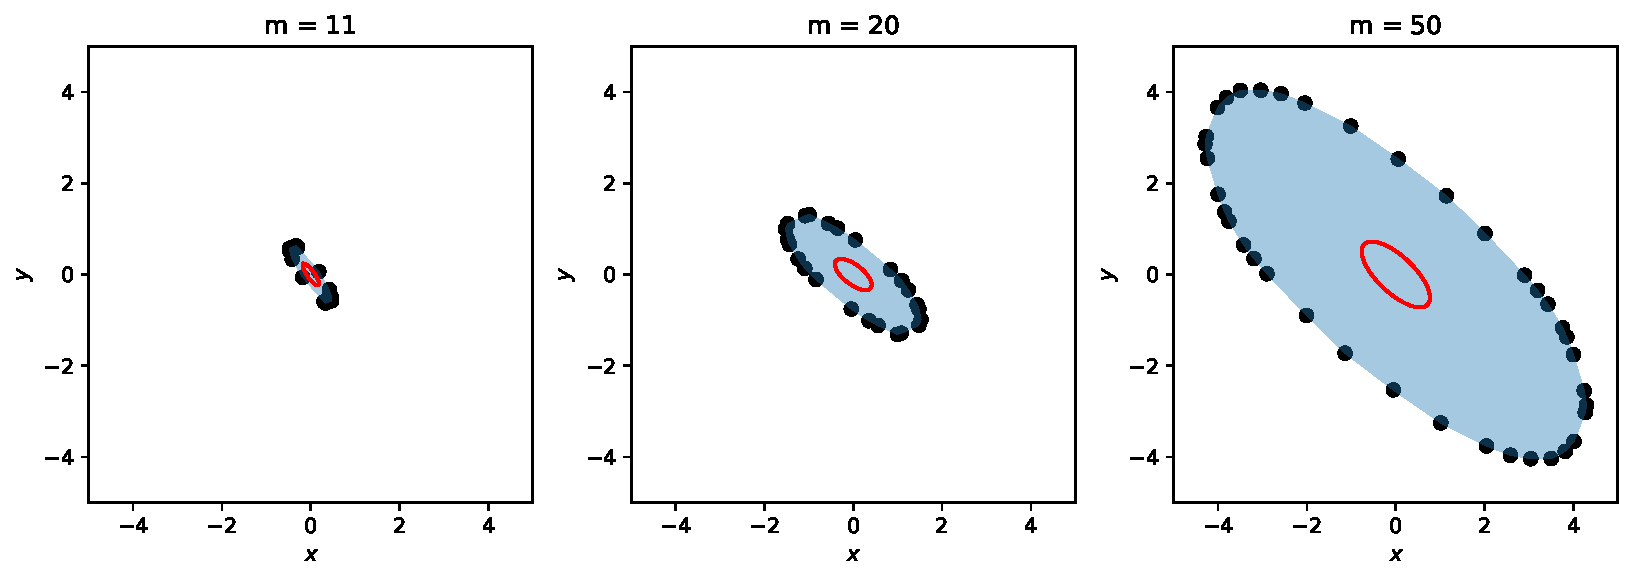
\includegraphics[trim={0 0 0 20},clip, width=0.9\linewidth]{img/chapter_3/ellipsoids_size.pdf}
  \end{minipage}
  
  \caption{Randomly generated force feasible sets using a hyperspherical (red ellipsoids) or hypercubic (blue polytopes) tension feasible set in $m$ dimensions. The volume of the force feasible set appears to depend on both the dimension and the shape of the tension feasible set.}
  \label{fig:ellipsoid_scale}
\end{figure}

To explain this phenomenon, consider that we aim to approximate force polytopes with ellipsoids. This necessitates scaling the ellipsoid by a factor that appears to depend on the dimension of the tension feasible set. Since the size of a vector relates to the concept of volume, there is an inherent connection between the size of the tension feasible set and the volume of the resulting force feasible set.

To formalize this, consider the unit $2$-ball $\mathcal{B}_2^m$ (a Euclidean ball of radius 1) and the unit $\infty$-ball $\mathcal{B}_{\infty}^m$ (a cube with edge length 2) in $\mathbb{R}^m$.  For $n < m$, let $\psi: \mathbb{R}^m \rightarrow \mathbb{R}^n$ be a surjective linear map of rank $n$ representing the projection from the tension space to the torque space.

For real Banach spaces, John's theorem (\cite{johnExtremumProblemsWithInequalities1948}) states that $m^{-1/2}\mathcal{B}_{\infty}^m \subset \mathcal{B}_2^m \subset \mathcal{B}_{\infty}^m$, where $m^{-1/2}\mathcal{B}_{\infty}^m$ denotes the $\infty$-ball (cube) scaled by a factor of $m^{-1/2}$. Since linear (and affine) maps preserve set inclusions, we also have $m^{-1/2}\psi(\mathcal{B}_{\infty}^m) \subset \psi(\mathcal{B}_2^m) \subset \psi(\mathcal{B}_{\infty}^m)$. In essence, this means that the unit sphere in $\mathbb{R}^m$ can be enclosed within a scaled cube, and vice versa.

To ensure that the force ellipsoids and force polytopes have roughly the same volume, one might consider scaling the radius of the tension feasible set sphere to match the volume of the cube. In this case, the ratio between the volumes of the two tension feasible sets would be 1. To compute the required radius, let $V_2^m(R)$ denote the volume of the $m$-dimensional Euclidean ball of radius $R$:
\begin{align}
\label{formula_volume_nsphere}
  V_2^m(R) = \frac{\pi^{m/2}}{\Gamma\left(\frac{m}{2} + 1\right)}R^m
\end{align}
where $\Gamma$ is the Euler gamma function, which extends the factorial function to positive real numbers, with $\Gamma(n) = (n-1)!$ for positive integers $n$.

The volume $V_\infty^m(R)$ of an $m$-dimensional cube with edge length $2R$ is given by $V_{\infty}^m(R) = (2R)^m$.  To find the radius $R'$ of a sphere with the same volume as the unit cube, we solve $V_2^m(R') = V_{\infty}^m(1)$, which yields:
\begin{align}
\label{formula:cube_sphere_same_radius}
R' = \left(\frac{\Gamma\left(\frac{m}{2} + 1\right)}{\pi^{m/2}}V_{\infty}^m(1)\right)^{1/m} = \frac{2}{\sqrt{\pi}}\Gamma\left(\frac{m}{2} + 1\right)^{1/m}
\end{align}

However, as illustrated in Figure \ref{fig:ellipsoid_scale_same_volume}, the ratio between volumes is not necessarily preserved under a linear map.
\begin{figure}[!htb]
  \captionsetup{justification=centering}
    \centering
    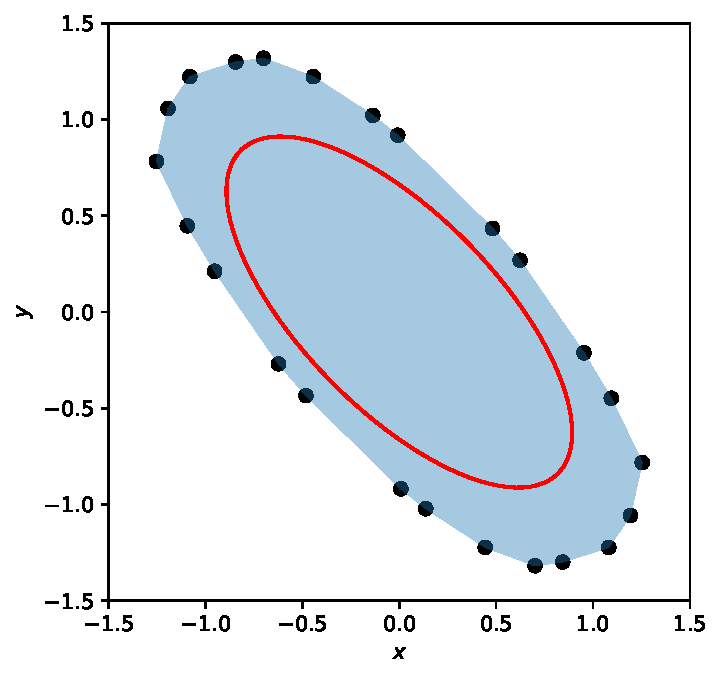
\includegraphics[trim={0 0 0 0},clip, width=0.5\linewidth]{img/chapter_3/myIma4_projection_cube_sphere_same_volume.pdf}  
  \caption{The force polytope (blue) is generated by randomly projecting a 20-dimensional unit cube with edge length 2 (volume $1048576$ N$^{20}$) onto a 7-dimensional space and intersecting with a random plane.  The force ellipsoid (red) is generated by applying the same projection-intersection operation to a sphere in $\mathbb{R}^{20}$ with radius $\frac{2}{\sqrt{\pi}}\Gamma\left(\frac{20}{2}+1\right)^{1/20}\sim 2.4012$, ensuring that its volume matches that of the cube. This figure clearly demonstrates that volumes are not preserved under the projection-intersection operation.}
  \label{fig:ellipsoid_scale_same_volume}
\end{figure}

This example illustrates that the \emph{shape} of the tension feasible set influences the volume of the force feasible set. It is important to recognize that volume is not a linear concept; it is not uniformly distributed within a space. Indeed, Formula \ref{formula:cube_sphere_same_radius} suggests that the volume of a cube is concentrated near its corners as its dimension increases, and this is a phenomenon emphasized in (\cite{milmanAsymptoticTheoryFinite2001}). If it lacked these corners (like a sphere), its volume would decrease with increasing dimensionality. This repartition of volume can be assimilated to the more physical concept of \emph{mass}. Essentially, this phenomenon states that the mass of objects in high dimensions is not reparted in a uniform manner, and this repartition is strongly linked to the shape of the considered object.

However, we must be cautious: the volume of a measurable set (a set for which the notion of volume is well-defined) depends not only on its shape but also on the chosen unit of measurement.  Conventionally, the unit of measurement is the $m$-dimensional cube with edge length 1.  This allows us to compare the volume of any measurable set to that of the unit cube.  More formally, this precise notion of volume is known as the \emph{Lebesgue measure} (\cite{lebesgueIntegraleLongueurAire1902}).

While convenient, this definition poses a challenge when considering transformations between spaces. The domain and codomain spaces may have different units of measurement, making direct comparisons of volumes problematic. As such, the determinant of a linear transformation can be interpreted as a measure of how the unit of measurement changes under the transformation.

A practical approach to address this issue is to embed both the domain ($\mathbb{R}^m$) and codomain ($\mathbb{R}^n$) within a larger ambient space with a unified notion of volume. However, these spaces can be equipped with different metrics (such as those induced by $p$-norms), which must be taken into account to understand how volume transforms between them.  The following paragraphs elaborate on this approach and demonstrate how it can be used to develop a computationally efficient method for approximating the projection of a unit $p$-ball with an ellipsoid.

\subsection{Leveraging the projected volume via the projection constant}
\label{subsec:projection_constant}
\emph{Projection constants} are a relatively recent concept in Banach space theory, first introduced in (\cite{murrayCOMPLEMENTARYMANIFOLDSPRO}). They remain an active area of research (\cite{donohoCountingFacesRandomlyProjected2010};\cite{foucartMaximalRelativeProjection2017}; \cite{bassoComputationMaximalProjection2019}; \cite{defantProjectionConstantsSpaces2022}) and aim to quantify the worst-case deformation of a unit ball under projection. 

More precisely, projection constants provide a way to determine the radius of a sphere that, when projected, yields a set with a volume comparable to that of a projected $p$-ball. This allows us to model the tension feasible set $\mathcal{T}$ as an ellipsoid or sphere that, when projected and/or intersected, produces a force feasible set with a volume similar to that obtained using the true shape of $\mathcal{T}$ under a $\mathcal{T}_p$ model. The key result regarding projection constants is that achieving this volume equivalence simply requires scaling the ellipsoid by a factor—the \emph{projection constant}—which depends on the choice of $p$.

If one wishes to model muscle independent tension interactions (represented by a cube-shaped tension feasible set), one can compute the force feasible set as an ellipsoid (using a sphere for the tension feasible set) and scale its radius by the appropriate projection constant. Different levels of interaction can be captured by varying the value of $p$ between 2 and $\infty$, corresponding to different shapes for the tension feasible set.

To compute these projection constants, we first need to introduce a few key concepts.

\paragraph*{Isometric embedding.} Let $X$ and $Y$ be Banach spaces. An operator $I: X \rightarrow Y$ is an \emph{isometric embedding} of $X$ into $Y$ if $I$ is injective, $I(X)$ is a subspace of $Y$, and $I(X)$ is isometric to $X$.  Essentially, an isometric embedding represents $X$ within a higher-dimensional space while preserving its metric structure, as we would simply represent a disc in a 3D space (\emph{i.e.} a 2-dimensional Euclidean space in a 3-dimensional Banach space equipped with its own unit ball).

\paragraph*{Projection.} For a subspace $X$ of $Y$, a \emph{projection} $P: Y \rightarrow X$ is an operator such that $P(x) = x$ for all $x \in X$.

\paragraph*{Projection constant.} For a subspace $X \subset Y$, the \emph{relative projection constant of $X$ in $Y$}, denoted by $\lambda(X, Y)$, is defined as:
\begin{align*}
\lambda(X, Y) = \inf\{\|P\|_{op} \mid P: Y \rightarrow X \text{ is a projection}\}
\end{align*}

Projection constants play a role in approximation theory. As noted in (\cite{defantProjectionConstantsSpaces2022}), for a projection $P: Y \rightarrow X$ and any $y \in Y$, the approximation error $\|y - P(y)\|_Y$ satisfies:
\begin{align*}
\|y - P(y)\|_Y \leq (1 + \|P\|_{op}) d(y, X)
\end{align*}
where $d(y, X) = \inf_{x \in X} \|y - x\|_Y$ is the distance from $y$ to $X$. To approximate $X$ by $Y$, or equivalently, to approximate the unit ball of $X$ by the unit ball of $Y$, the operator norm $\|P\|_{op}$ should be minimized. This minimum is achieved when $\|P\|_{op} = \lambda(X, Y)$.

Therefore, we focus on the worst-case scenario, represented by the largest possible value of $\|P\|_{op}$. This value quantifies the maximal dilation of vectors in the unit ball of $Y$ when projected onto $X$.  This is known as the \emph{(absolute) projection constant} of $X$, denoted by $\lambda(X)$, and is defined as:
\begin{align*}
\lambda(X) = \sup \lambda(I(X), Y)
\end{align*}
where the supremum is taken over all Banach spaces $Y$ containing an isometric copy of $X$ and over all isometric embeddings $I: X \rightarrow Y$. In essence, we embed the unit ball of $X$ into higher-dimensional spaces and assess the worst-case deformation of these embeddings under projection onto $X$.

A key result in Banach space theory states that any finite-dimensional Banach space $X$ can be isometrically embedded into a finite-dimensional space equipped with the $\infty$-norm \cite{defantProjectionConstantsSpaces2022}. In other words, we can always find a higher-dimensional cube with a section or projection that is a linear transformation of a unit $p$-ball. This implies that finding the absolute projection constant $\lambda(X)$ is equivalent to finding the minimal projection constant from a finite-dimensional space with the $\infty$-norm onto $X$.

Intuitively, the projection constant $\lambda(X)$ can be interpreted as a measure of the maximal distortion (in terms of volume) when projecting a $p$-ball onto $X$.
% Once this metric is retrieved, we shall take this second $p$-ball and multiply it by the computed value to obtain a worst-case approximation (in size) of the first projected $p$-ball. In practice in the context of choosing a modeling for the tension feasible set $\mathcal{T}$, it tells us that whatever the choice of $p$ for $\mathcal{T}_p$, we can adapt the size of the torque feasible set (in volume) afterwards to fit another chosen $p$. Let's recall that the choice of $p$ can be seen as how the working biomechanician or robotician would choose to model the interactions between muscle tensions.

Since there are infinitely many projections, isometric embeddings, and also higher-dimensional Banach spaces, a central focus of projection constant theory is to compute bounds or exact values for specific cases.  Even today, determining projection constants remains an active area of research (\cite{deregowskaSimpleProofGrunbaum2023}; \cite{defantProjectionConstantsSpaces2022}; \cite{deregowskaValueFifthMaximal2022}; \cite{chalmersMINIMALPROJECTIONSABSOLUTEPROJECTION}; \cite{bassoComputationMaximalProjection2019}; \cite{foucartMaximalRelativeProjection2017}).

We are particularly interested in the projection constants of $\ell_p^n$ spaces, which represent $\mathbb{R}^n$ equipped with the $p$-norm $\|\cdot\|_p$. These spaces correspond to different shapes for the tension feasible set. The following theorem summarizes several decades of results on the projection constants of $\ell_p^n$ spaces:

\begin{theorembox}{Projection Constants of $\ell_p^n$ Spaces}{proj_constant_lp_spaces}
  Let $\ell_p^n$ be the finite-dimensional normed space $\mathbb{R}^n$ equipped with the $p$-norm $\|\cdot\|_p$, defined for all $x\in \ell_n^p$ as $\|x\|_p=\left(\sum_{i=1}^n \vert x_i \vert^p\right)^{1/p}$. Let $\lambda(\ell_p^n)$ denote the projection constant of $\ell_p^n$. Then:

  \vspace{5mm}

  \begin{itemize}
    \item \underline{For $p=2$:}
    \begin{align*}
            \lambda(\ell_2^n) = \frac{2}{\sqrt{\pi}}\frac{\Gamma(\frac{n}{2} + 1)}{\Gamma(\frac{n}{2} + \frac{1}{2})}
            \end{align*}
    where $\Gamma$ is the Euler gamma function, defined for all $z \in \mathbb{C}$ with a strictly positive real part as $\Gamma(z)=\int_0^{+\infty}t^{z-1}e^{-t}\,dt$.
    \item \vspace{5mm} \underline{For $p=1$:}
    \begin{align*}
            \lambda(\ell_1^n) = \begin{cases} 
               \lambda(\ell_2^{n-1}), & \text{if $n$ is even} \\
               \lambda(\ell_2^n), & \text{if $n$ is odd}
             \end{cases}
            \end{align*}
    \item \vspace{5mm} \underline{For $2<p<\infty$:}
    \begin{align*}
            \lambda(\ell_p^n) = O(n^{\frac{1}{p}})
            \end{align*}
      where $O$ is the Big O notation describing asymptotic growth.
    \item \vspace{5mm} \underline{For $1<p<2$:}
    \begin{align*}
            \lambda(\ell_p^n) \approx \sqrt{\frac{2n}{\pi}}\quad \text{as $n\rightarrow +\infty$}
            \end{align*}
  \end{itemize}
\end{theorembox}
\begin{proof}
  The cases $p=1$ and $p=2$ were proven in (\cite{grunbaumProjectionConstants1960}). The asymptotic bound for $2<p<\infty$ was proven in (\cite{gordonProjectionMacphailConstants1968} and \cite{garlingRelationsConstantsAssociated1971}). The approximation for $1<p<2$ was derived in (\cite{konigProjectionConstantsSymmetric1999}).
\end{proof}

Note that the values provided in this theorem apply only to real normed spaces. For complex normed spaces, the corresponding projection constants can be found in (\cite{defantProjectionConstantsSpaces2022}).

To conclude this subsection, let's consider Figure \ref{fig:example_proj_constant_applied}, which illustrates an approximation of a zonotope generated with a large number of generators by an ellipsoid. This ellipsoid is computed using the projection constant $\lambda(\ell_2^{m})$ for $m = 11$, 20, and 50.  This is equivalent to approximating a $\mathcal{T}_{\infty}$ model with a $\mathcal{T}_2$ model by simply scaling the ellipsoid with the factor $\lambda(\ell_2^{m})$.
\begin{figure}[!htb]
    \captionsetup{justification=centering}
    \begin{minipage}{1\linewidth}
        \centering
        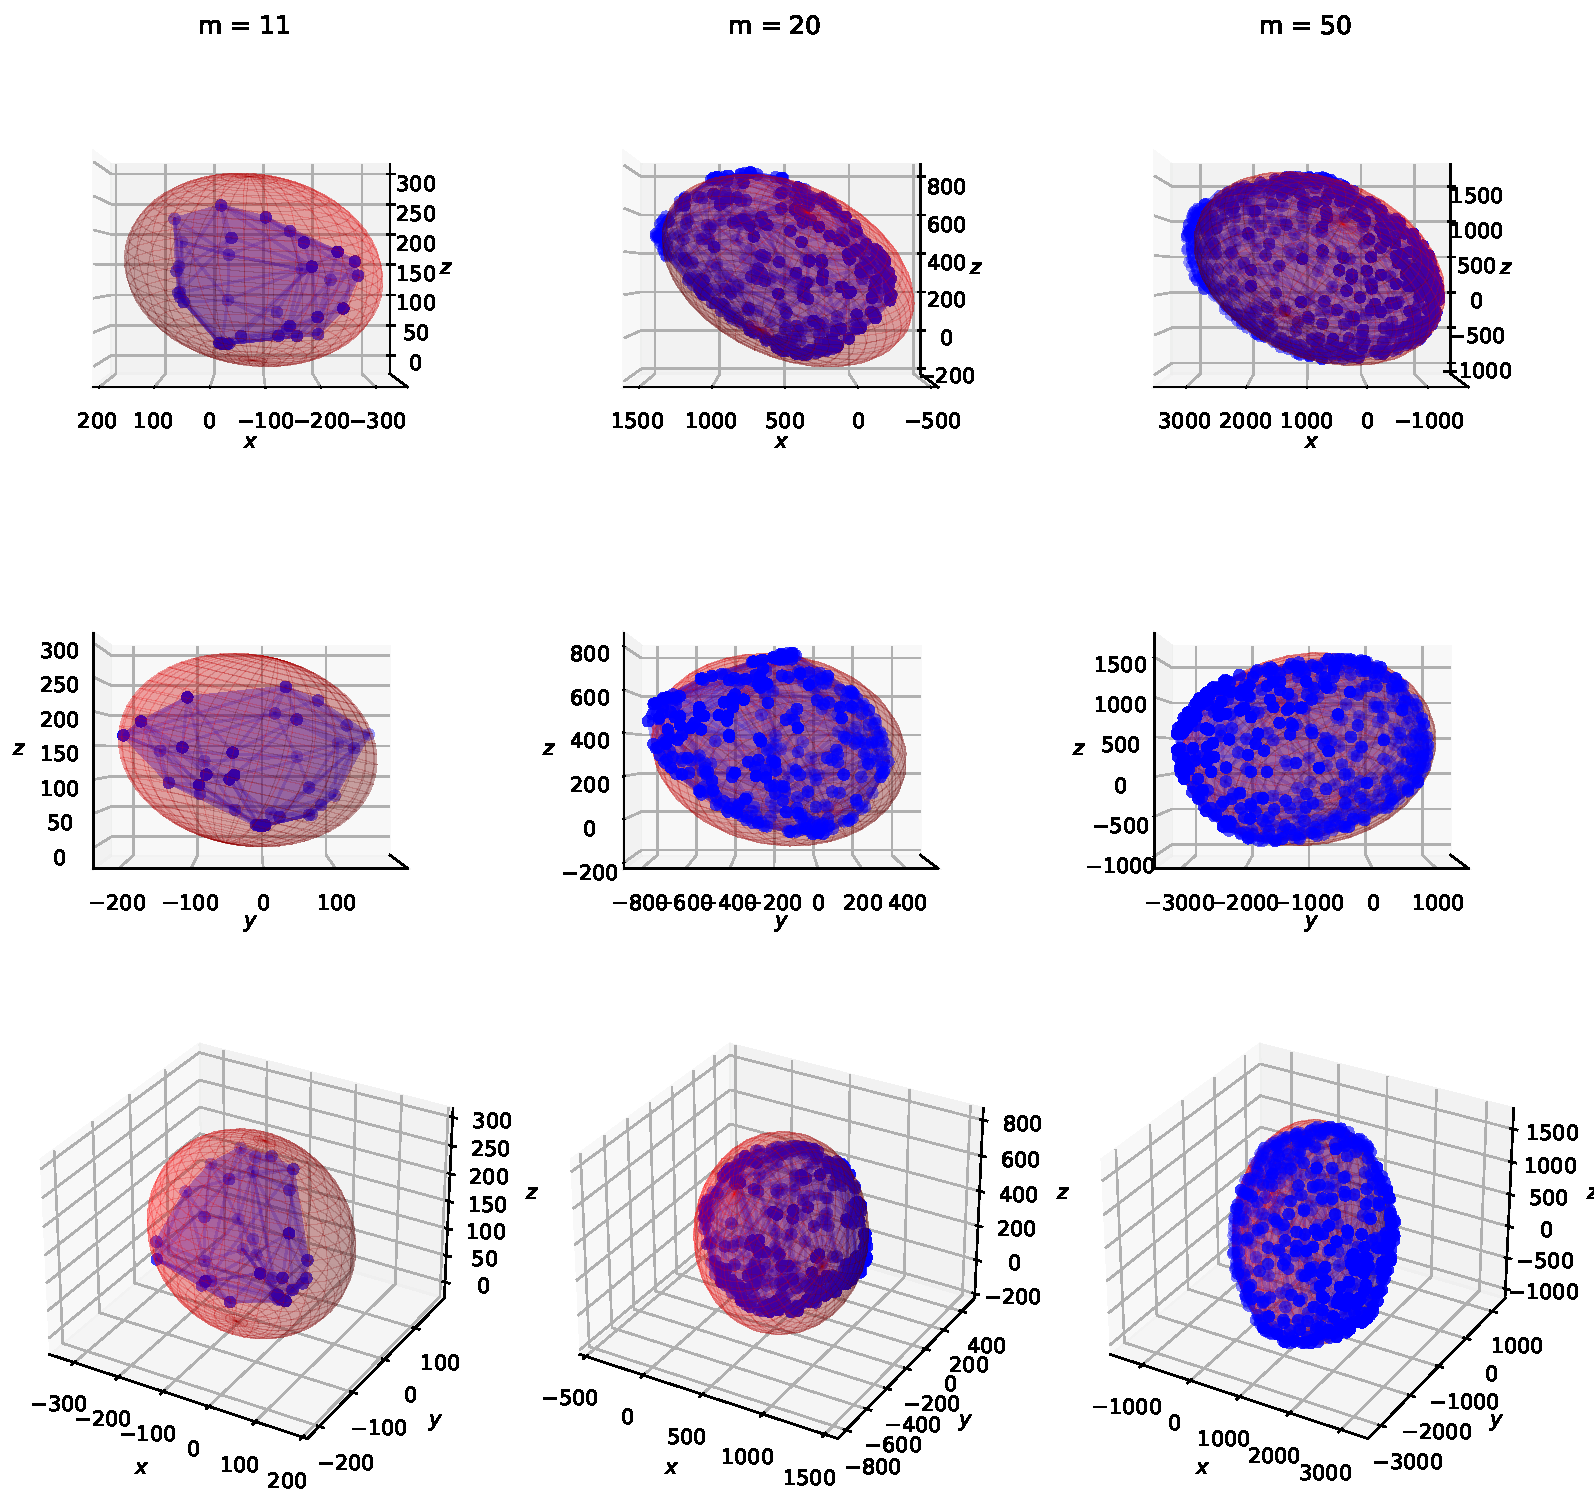
\includegraphics[trim={0 700 0 0},clip, width=0.9\linewidth]{img/chapter_3/myIma5_projection_constant.pdf}
    \end{minipage}
    \begin{minipage}{1\linewidth}
        \centering
        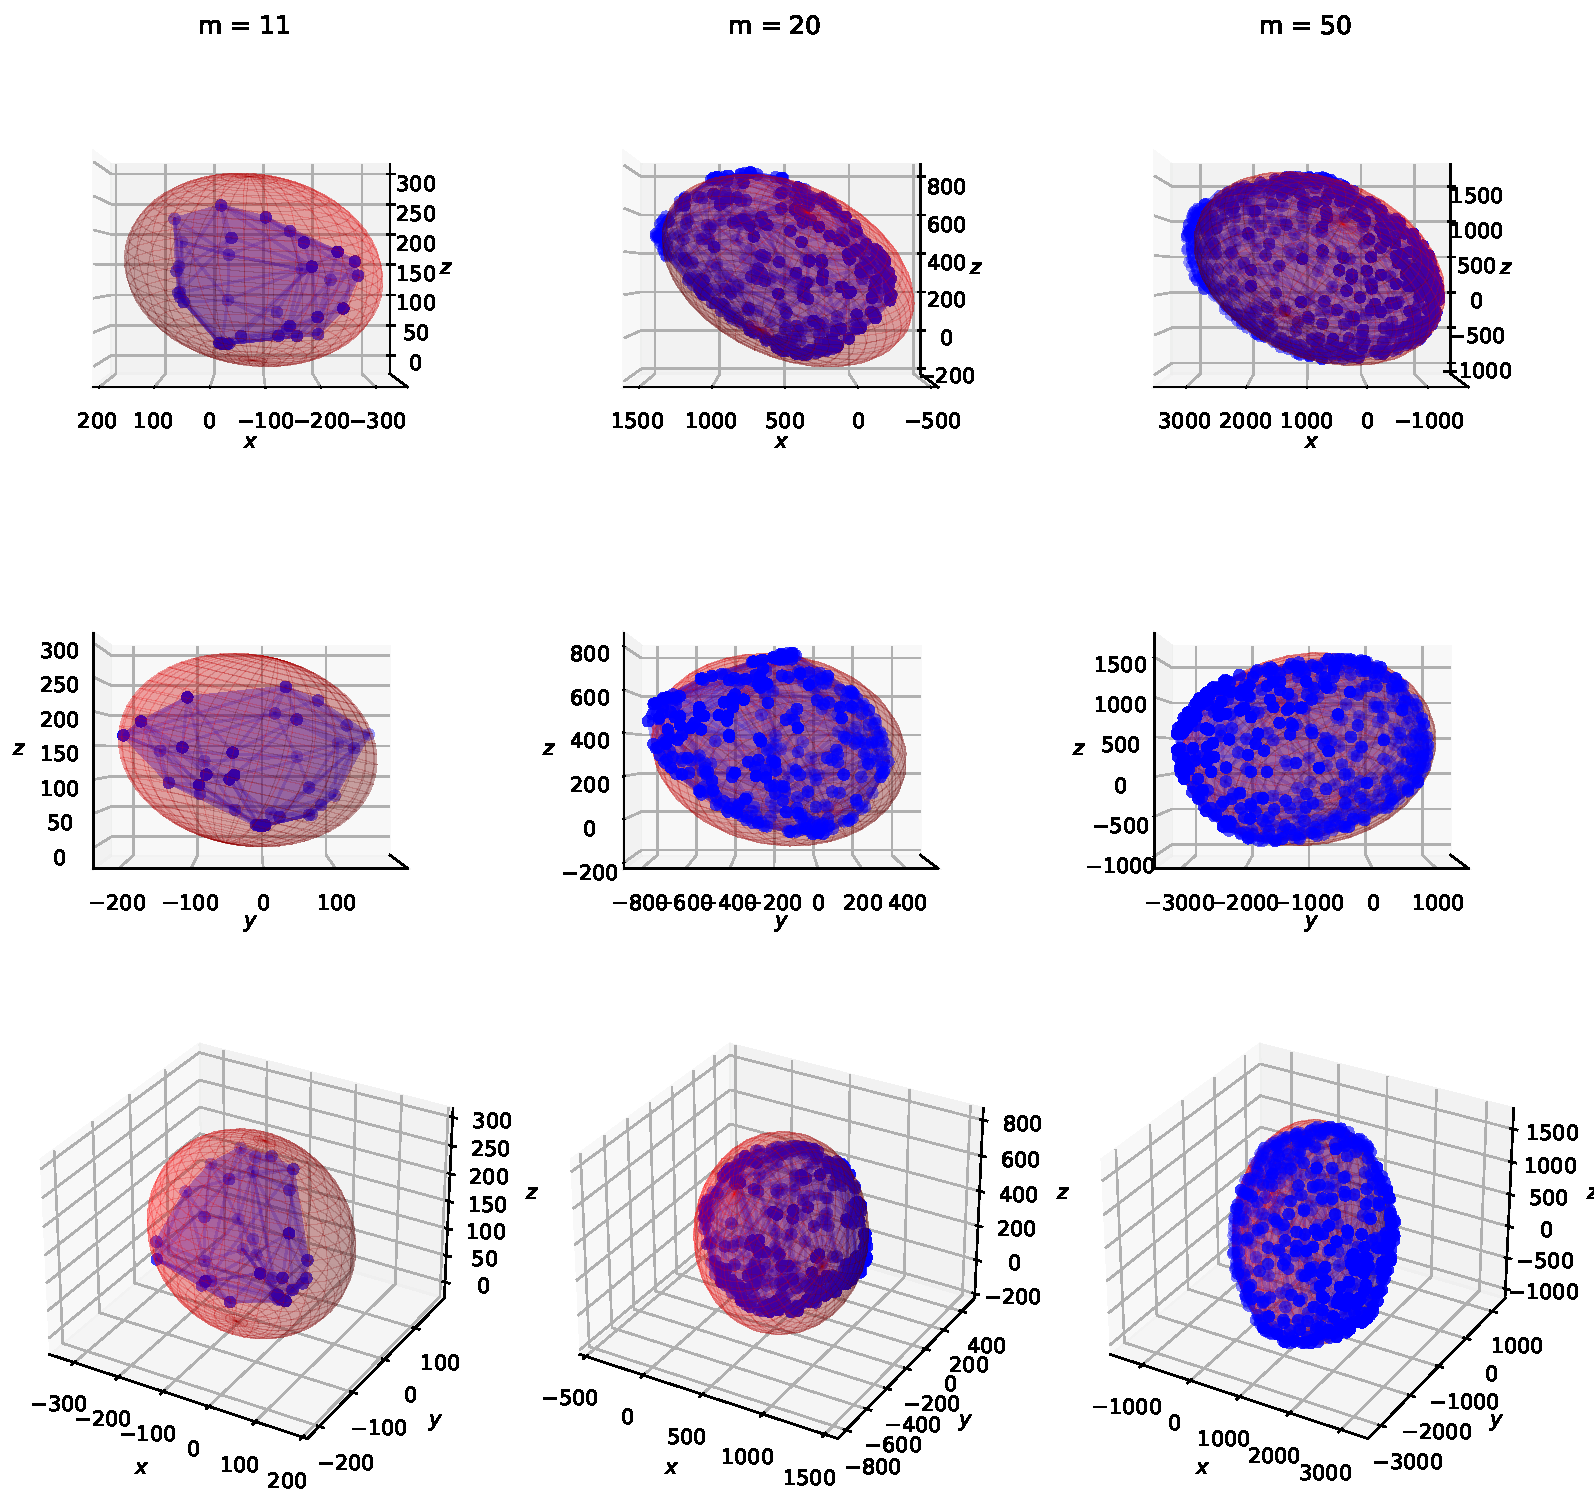
\includegraphics[trim={0 500 0 60},clip, width=0.9\linewidth]{img/chapter_3/myIma5_projection_constant.pdf}
    \end{minipage}
    \begin{minipage}{1\linewidth}
        \centering
        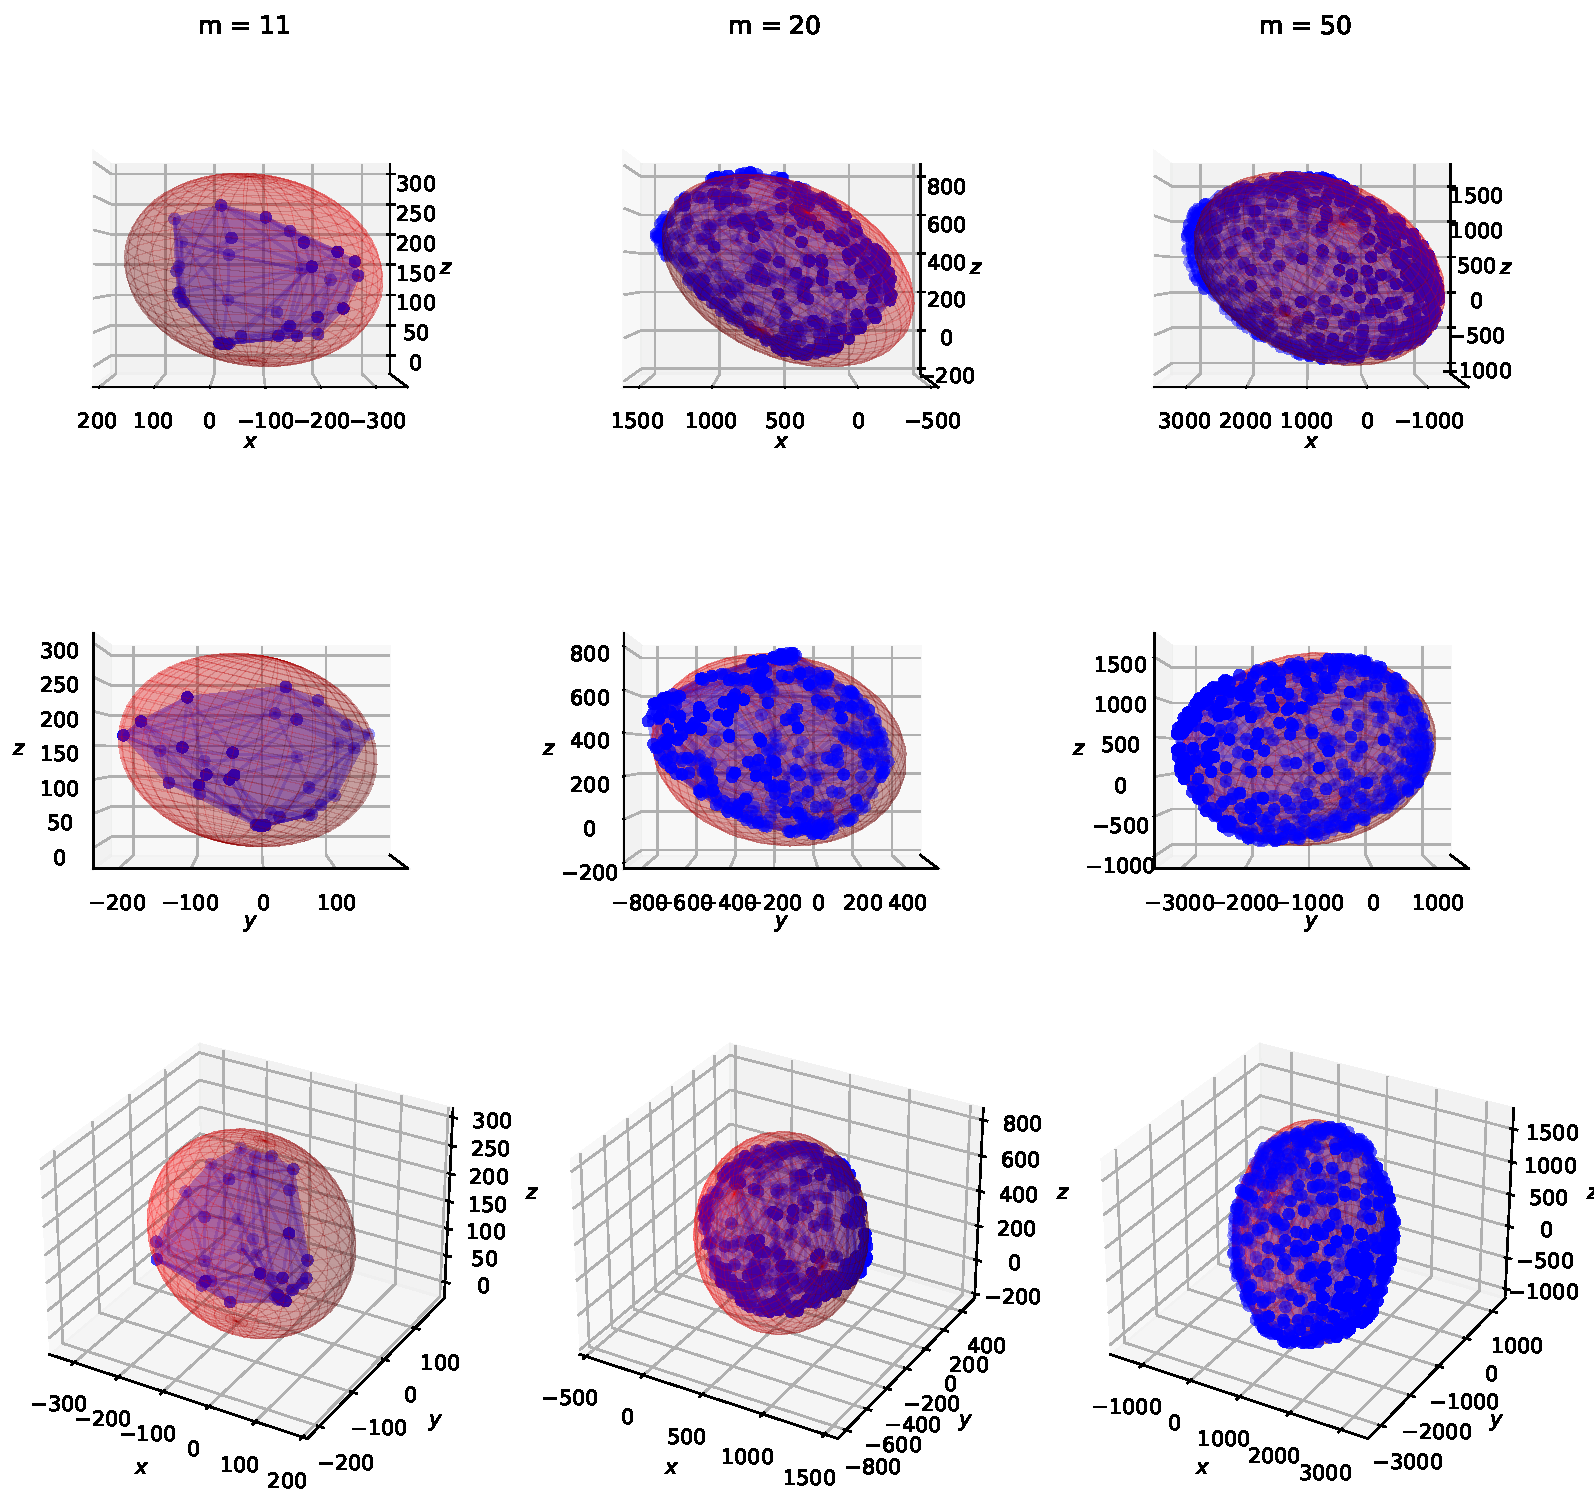
\includegraphics[trim={0 255 0 300},clip, width=0.9\linewidth]{img/chapter_3/myIma5_projection_constant.pdf}
    \end{minipage}
    \begin{minipage}{1\linewidth}
        \centering
        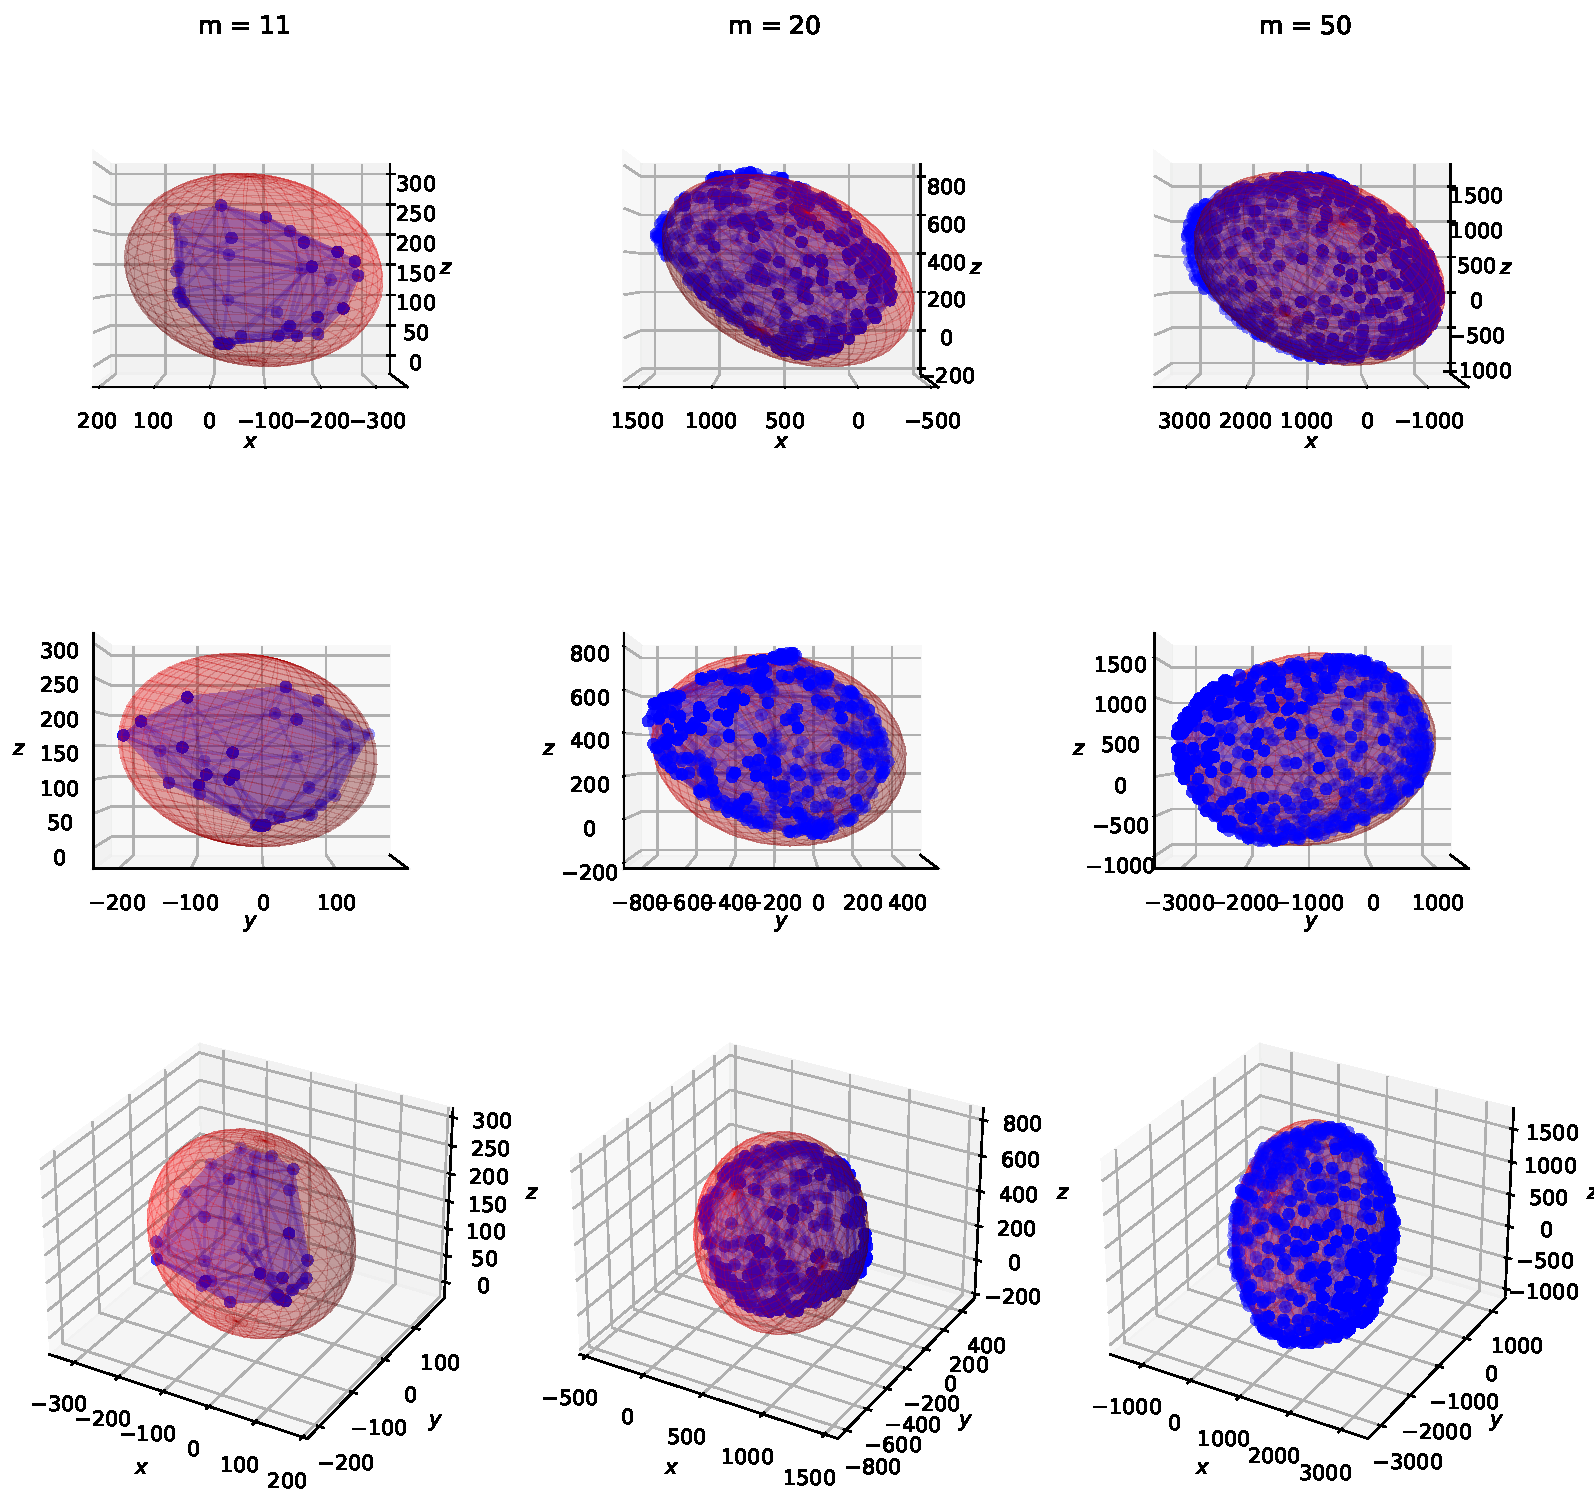
\includegraphics[trim={0 0 0 500},clip, width=0.9\linewidth]{img/chapter_3/myIma5_projection_constant.pdf}
    \end{minipage}
    
    \caption{Each column represents a different number of muscles ($m = 11$, 20, and 50). The force polytopes (blue) are generated by randomly projecting an $m$-dimensional cube with edge length 1000 onto a 7-dimensional torque space and intersecting with a random 3D subspace. As the number of muscles increases, the ellipsoidal approximation (red), computed using the projection constant $\lambda(\ell_2^m)$, becomes more accurate and accounts for the increasing volume of the tension feasible set. This improvement with increasing $m$ is consistent with the asymptotic nature of projection constants.
    }
    \label{fig:example_proj_constant_applied}
\end{figure}

\section{Quantifying the impact of muscle geometry on maximum joint torque generation}
\label{sec:sensitivity}
This section presents a novel application of the theoretical framework developed in this chapter to quantify the influence of muscle geometry (or muscle path descriptions) on the force feasible set. As demonstrated in the preceding sections, a large number of muscles leads to an ellipsoidal force feasible set, and we have established computationally tractable methods for approximating this ellipsoid.

Muscle geometry is subject-specific. When scaling a generic musculoskeletal model, a common approach is to adjust bone lengths and reposition muscle path points accordingly. However, in our non-in vivo context, we question the necessity of adapting these path points.  Our goal is to quantify the impact of muscle geometry on the force feasible set.

To address this, we adopt a practical approach using Holzbaur's upper limb musculoskeletal model (\cite{holzbaurModelUpperExtremity2005}), which has 7 degrees of freedom describing the shoulder, elbow, and wrist joints. This model comprises 50 muscles, each with 2 to 12 path points defined in OpenSim. Each point has a default position relative to a reference frame.

Our methodology is straightforward. For a set of joint configurations, we perturb the location of each muscle path point by sampling from a uniform distribution within a 0.005-meter radius of its default location. This is equivalent to uniformly sampling points within a cube with edge length 0.01 centered at the default location.

Given the large number of muscles, we can model the tension feasible set as a transformation of a unit sphere (an ellipsoid). For each joint configuration, we assume a unit sphere in $\mathbb{R}^{50}$ for the tension feasible set. The radius is normalized because we are interested in how the metric of the tension feasible set is maximally deformed by variations in muscle geometry. To analyze the metric of the force feasible set, we utilize its reformulation as an \emph{intersection followed by projection}, as described in Section \ref{sec:ellipsoidal_shape_ffs}. In this framework, the unit ball of the force feasible set is obtained by intersecting the tension feasible set sphere with the subspace $K$, resulting in an ellipsoid, which is then projected onto $\im J^T$ via the lever arm matrix.  The operator norm quantifies this metric deformation in the worst-case scenario. Since we are considering a deformation from a sphere to an ellipsoid, the computation involves the 2-norm of the generators of the resulting ellipsoid.

The following table presents the 2-norm computations for 100 random variations of each muscle path point in Holzbaur's model, across four different postures. These postures are defined in degrees for the 7 generalized coordinates parameterizing the upper-limb joint rotation axes as follows:
\begin{itemize}[noitemsep]
    \item {$\mathbf{q}_1 = (13,12.5,-41,30.5,-5.3,0.19,-0.76)$}
    \item {$\mathbf{q}_2 = (13,90,-41,30.5,-5.3,0.19,-0.76)$}
    \item {$\mathbf{q}_3 = (37,90,21,30.5,-5,0.19,-0.76)$}
    \item {$\mathbf{q}_4 = (37,31,21,30.5,-1.3,0.19,-0.76)$}
    \item {$\mathbf{q}_5 = (37,31,21,76,42,0.19,-0.76)$}
    \item {$\mathbf{q}_6 = (110,31,21,76,42,0.19,-0.76)$}
    \item {$\mathbf{q}_7 = (110,10,21,76,74,0.19,-0.76)$}
    \item {$\mathbf{q}_8 = (96,79,120,76,74,0.19,-0.76)$}
\end{itemize}

\begin{table}[!ht]
    \centering
    \begin{tabular}{|c||c|c|}
    \hline
    Posture & \makecell{Mean of $2$-norm} & Standard deviation of $2$-norm \\
    \hline
    \hline
    $\mathbf{q}_1$ & $0.1140$ & $0.0021$ \\ \hline
    $\mathbf{q}_2$ & $0.0822$ & $0.0055$ \\ \hline
    $\mathbf{q}_3$ & $0.0953$ & $0.0012$ \\ \hline
    $\mathbf{q}_4$ & $0.0843$ & $0.0017$ \\ \hline
    $\mathbf{q}_5$ & $0.0929$ & $0.0012$ \\ \hline
    $\mathbf{q}_6$ & $0.0749$ & $0.0028$ \\ \hline
    $\mathbf{q}_7$ & $0.0859$ & $0.0019$ \\ \hline
    $\mathbf{q}_8$ & $0.0980$ & $0.0018$ \\ \hline
    \end{tabular}
    \caption{Mean and standard deviation of the 2-norm of the force feasible set, computed as an intersection followed by a projection of the tension ellipsoid. Each data point represents 100 random variations of the initial coordinates of each muscle path point in Holzbaur's upper limb musculoskeletal model.}
    \label{tab:sensitivity}
\end{table}

The key result here is the standard deviation: the closer it is to 0, the less impact muscle geometry has on the deformation of the tension feasible set. This is a set-theoretic interpretation, focusing on the overall deformation of the entire set rather than individual muscle tension combinations.

While almost all standard deviations are close to zero, we recall that we are working with a normalized tension feasible set (a unit sphere). Therefore, the magnitudes of the values are inherently less than 1. These low means reflect the projected volume phenomenon: a sphere in 50 dimensions has a small volume even if its vectors have a norm of 1. Consequently, the force feasible ellipsoid inherits this low volume, resulting in small vector magnitudes. This highlights the importance of carefully considering the order of magnitude when interpreting the values in this table.

For instance, consider the first posture, $\mathbf{q}_1$. The mean indicates that, on average, across all muscle path point variations, a combination of muscle tensions totaling 1 N corresponds to a maximum torque of approximately 0.1140 Nm in the worst-case scenario. In simpler terms, the tension exerted by the muscles can account for, at most, about 11\% of 1 Nm on average.

Now, assume that each muscle can exert a maximum tension of 1000 N, and consider arbitrary combinations of muscle activations. The standard deviation represents the worst-case variation in the size (2-norm) of a tension vector when transformed into the torque space. This means that muscles collectively exerting 1000 N produce a torque with a magnitude between $1000 \times (0.1140 - 0.0021) = 111.9$ Nm and $1000 \times (0.1140 + 0.0021) = 116.1$ Nm.  Therefore, even with precise personalization of muscle geometry, the resulting force feasible set in the torque space would exhibit a maximal size difference of only $116.1 - 111.9 = 4.2$ Nm in posture $\mathbf{q}_1$.

Let's summarize these worst-case scenarios in the following table:

\begin{table}[!ht]
    \centering
    \begin{tabular}{|c||c|c|}
    \hline
    Posture & \makecell{Worst size difference \\ using max-min} & \makecell{Maximal torque contribution difference \\ between two geometries if \\ all muscles have a tension of $1000$N} \\
    \hline
    \hline
    $\mathbf{q}_1$ & $0.0099$ & $9.9$ Nm \\ \hline
    $\mathbf{q}_2$ & $0.0554$ & $55.4$ Nm \\ \hline
    $\mathbf{q}_3$ & $0.0066$ & $6.6$ Nm \\ \hline
    $\mathbf{q}_4$ & $0.0091$ & $9.1$ Nm \\ \hline
    $\mathbf{q}_5$ & $0.0055$ & $5.5$ Nm \\ \hline
    $\mathbf{q}_6$ & $0.0131$ & $13.1$ Nm \\ \hline
    $\mathbf{q}_7$ & $0.0084$ & $8.4$ Nm \\ \hline
    $\mathbf{q}_8$ & $0.0098$ & $9.8$ Nm \\ \hline
    \end{tabular}
    \caption{Worst-case difference in the 2-norm of a muscle tension vector projected onto the force feasible set (expressed in the torque space) due to variations in muscle geometry. Each value is computed using the range of observed 2-norms across 100 random variations of muscle path points.}
    \label{tab:sensitivity2}
\end{table}

These results provide valuable insights into how variations in muscle geometry affect the range of achievable joint torques, particularly when considering different postures.

In our context, with a spherical tension feasible set, these findings allow us to utilize Holzbaur's default muscle path points for specific postures while understanding the potential deviations from a more personalized musculoskeletal model. This assumption will be studied in more details in Chapter \ref{chapter:4}.

Quantifying the error introduced by our assumptions on the modeling of tension feasible sets. As such, we propose an index that specifically measures the contribution of muscle geometry to the force feasible set (expressed in the torque space) deriving from a chosen $\mathcal{T}$ model.

Furthermore, we hypothesize that increasing the number of muscles should reduce the sensitivity of the force feasible set to variations in muscle geometry. Intuitively, as the number of muscles increases, both the force and torque feasible sets tend towards an ellipsoidal shape. From a metric perspective, this implies that the influence of individual muscles on the torque space diminishes, leading to a reduced overall impact of muscle geometry variations. We also conjecture that with an infinite number of muscles, the projection from the tension space to the torque space becomes increasingly independent of muscle geometry. This does not imply that muscle geometry is irrelevant, but rather that there exists a global projection (depending on muscle geometry) that maps the tension feasible set directly to the force feasible set without explicitly considering the intermediate torque space, and bypassing any intersection step.

Our reformulation of the force feasible set as an intersection followed by a projection provides some clues about this hypothetical projection. Recall that the tension feasible set (in $\mathbb{R}^m$) is first intersected with a subspace $K$ of dimension $m - (n - p)$. When the number of muscles is large, this intersection has minimal impact. The subsequent projection, however, depends on muscle geometry (since it requires the lever arm matrix). If we assume that all muscle geometries project similarly through a matrix $P \in \mathbb{R}^{n \times m}$ (i.e., all muscles have a similar degree of influence on the force feasible set metric), then the direct link between the tension and force spaces would be $(J^T)^+ P(\mathcal{T})$. In this scenario, only the mean muscle tension, arm geometry, and posture would be the determining factors. Chapter \ref{chapter:5} will explore this assumption further in the context of predicting force feasible sets for individuals, to argue that these theoretical hypotheses may not hold in regard to experimental measurements of maximal isometric forces.

\section{Conclusion}
\label{sec:approx_discussion}

The objective of this chapter was to gain a deeper set-theoretic understanding of the relationships between the elements in the formulation of the force feasible set, $\mathcal{F}$, initially described as:
\begin{align*}
\mathcal{F} = \left\{ \mathbf{f}\in \mathbb{R}^p \mid \exists \mathbf{t}\in\mathcal{T},\quad J^T\mathbf{f} = -L^T\mathbf{t} - \mathbf{G} \right\}
\end{align*}

More abstractly, this can be expressed in terms of a surjective affine map $\psi: \mathbb{R}^m \rightarrow \mathbb{R}^n$ and an injective linear map $\phi: \mathbb{R}^p \rightarrow \mathbb{R}^n$:
\begin{align*}
\mathcal{F} = \im \phi \cap \psi(\mathcal{T})
\end{align*}

While this geometric perspective clarifies the operations involved, it is essential to consider the underlying physics. The unit of measurement used to describe elements of $\mathcal{F}$ is derived from a transformation of the unit of measurement of the tension feasible set, $\mathcal{T}$. This connection between geometry and metric is the subject of Banach space theory. By exploring the Local Theory of Banach spaces and reformulating $\mathcal{F}$, we argued that, regardless of the choice of $\mathcal{T}$, there is a strong probability that the shape of $\mathcal{F}$ should to be ellipsoidal if a large number of muscles is considered in the modeling of an \emph{in silico} upper-limb using a musculoskeletal model. Generally, ellipsoids offer computational advantages for set representation and analysis, as we will see in Chapter \ref{chapter:4}, it is easier to compare two ellipsoids than two polytopes.

However, explicitly computing this approximating ellipsoid is not straightforward. We observed a relationship between the volumes of projected spheres and projected cubes, mediated by the dimension of the tension feasible set (i.e., the number of muscles). This relationship is quantified by the \emph{projection constant}, $\lambda$, which indicates the scaling factor required for a sphere to have a volume comparable to that of a cube of the same dimension. From a metric perspective, it expresses how the unit of force in the tension feasible set (Newtons) relates to the unit of torque (Newton-meters).

This metric perspective enables us to directly quantify the influence of muscle geometry on the force feasible set using the operator norm of $-L^T$, particularly when the number of muscles is large compared to the dimension of the torque space. As an application, we can analyze how small variations in muscle paths affect this norm for a given posture. If the range of these norms is below a context-dependent threshold, we can assess the necessity of personalizing muscle geometry when studying force and torque feasible sets in isometric conditions.

In summary, Section \ref{sec:ellipsoidal_shape_ffs} established that the force and torque feasible sets tend to have an ellipsoidal shape when a large number of muscles are involved. Section \ref{sec:projected_volume_problem} demonstrated how to compute an ellipsoidal approximation based on the number of muscles and the degree of tension interaction. Finally, Section \ref{sec:sensitivity} analyzed the influence of various factors on the force feasible set, including posture, muscle geometry, muscle tensions, and their interactions.  It was shown that interactions primarily affect the global shape, posture determines the global orientation, and muscle tensions, muscle geometry, and muscle number collectively influence the global size. To isolate the impact of muscle geometry, an index related to the operator 2-norm of $-L^T$ can be utilized, particularly when the number of muscles is large enough to warrant an ellipsoidal approximation.

The theoretical framework developed in this chapter enhances our understanding of the underlying structure of muscle tension capabilities inscribed in our approach of \emph{in silico} force feasible sets. Chapter \ref{chapter:4} will explore these results \emph{in silico}, demonstrating how ellipsoidal approximations can be used to personalize muscle parameters in a musculoskeletal model based on force production capabilities. Building on these investigations, Chapter \ref{chapter:5} will then incorporate experimentally measured maximal isometric forces to evaluate the validity of the ellipsoidal representation and its implications for the shape of the muscle tension feasible set.